% !TEX root=../../main_file.tex
% !TeX TS-program = pdflatex
% !TeX checkspelling = fr_toutesvariantes


\chapter{(Photo-)électrochimie \emph{in-situ} à haute température: conception, développement, validation de l'installation}
\label{chap:design}
\chaptermark{(Photo-)électrochimie \emph{in-situ} à haute température}
\begin{refsection}
\minitoc

\section{Introduction}
    Ce troisième chapitre est consacré au premier axe de notre travail portant sur la conception et le développement
    d'une nouvelle cellule électrochimique permettant de réaliser des mesures (photo-)électrochimiques \emph{in-situ} en 
    environnement REB.

    Le choix des sources d'illumination est présenté dans un premier temps ainsi que les deux manières d'illuminer
    les échantillons: \emph{illumination continue} et \emph{illumination modulée}.
    
    Ensuite la technique de caractérisation
    photoélectrochimique est abordée après un bref rappel des principes de cette technique avec une présentation
    détaillée du montage expérimental et des méthodes d'analyses des résultats. Dans cette partie, nous présenterons un
    travail original que nous avons mené pour estimer les incertitudes sur les largeurs de bande interdite déduites des
    ajustements numériques des spectres en énergie de photocourants au modèle développé par J.P. Petit \citep{Petit2013} au SIMaP pour des
    échantillons complexes.
    
    Les différents éléments de la cellule électrochimique développée sont décrits dans un troisième temps 
    ainsi que ceux d'une cellule complémentaire permettant de mesurer le flux de photons arrivant à la surface des
    échantillons.

    La partie suivante de ce chapitre est dédiée à l'intégration des sources d'illumination ainsi que des deux cellules
    dans la boucle de contrôle de la chimie de l'électrolyte. Cette partie apporte une vision d'ensemble
    du dispositif expérimental en
    termes d'alignement des cellules et des sources, de gestion de la température et de contrôle de la teneur en
    oxygène dissous. 


%%%%%%%%%%%%%%%%%%%%%%%%%%%%%%%%%%%%%%%%%%%%%
\section{Source d’illumination}\label{sec:ch3_UV_sources}

    Il a été suggéré au chapitre \ref{chap:ch1_bib} qu'une illumination UV pouvait être un moyen de simuler
    partiellement l’effet des irradiations en réacteur REB
    en s’affranchissant des contraintes de sécurité liées aux rayonnements plus intenses tels que les rayonnements
    $\gamma$
    ou les rayonnements neutroniques. 
    De plus, les caractérisations photoélectrochimiques permettent d'étudier les couches
    d'oxydation en tirant parti des propriétés semiconductrices des oxydes.
    L'illumination peut donc être utilisée pour exciter fortement la couche d'oxyde mais également pour caractériser
    cette dernière.
    La figure \ref{fig:ch3_UV_sources_use} schématise les deux manières envisagées pour utiliser l'illumination:
    1) illumination intense et continue, 2) illumination modulée. 
    
    \begin{figure}[H]
		\centering
		
\includegraphics[width=0.65\textwidth]{schematic_diagram_two_aspects_PEC_Photolysis.png}
		\caption{Représentation schématique des intérêts de l'illumination.}
		\label{fig:ch3_UV_sources_use}
	\end{figure}

    
    L'illumination intense permet de quantifier les modifications du
    comportement électrochimique des oxydes formés sur les alliages Zy2 et Inc718 avec les méthodes électrochimiques
    classiques décrites au chapitre \ref{chap:methods}.   
    Initialement, cette illumination intense dans le domaine des UV devait être assurée par un laser gaz pulsé (HeAg)
    fourni par \emph{Laser2000} 
    ayant une longueur d’onde de travail de \SI{224}{\nano\meter} avec une puissance de pulse de \SI{10}{\milli\watt}
    et un diamètre de faisceau de \SI{3}{\milli\meter} pour une puissance moyenne d'environ
    \SI{85}{\micro\watt\per\square\centi\meter}. 
    L’énergie associée à cette longueur d'onde, soit \SI{5.5}{\electronvolt}, est supérieure à la largeur
    de bande interdite de la zircone (\SI{5}{\electronvolt}).
    La photolyse de l’eau dans le volume est difficilement réalisable à 
    cette longueur d’onde \citep{Mozumder2002} mais une photolyse assistée en surface 
    de l’oxyde de zirconium, par l'intermédiaire de trous photogénérés dans sa bande de valence, est envisageable
    \citep{Takahashi2006, Petrik2001}.
    
    Cependant, les premiers essais d'illumination à \SI{280}{\degreeCelsius} ont montré que le laser pulsé n'était
    pas assez puissant pour engendrer de fortes modifications en termes de potentiel électrochimique, courant de couplage
    et courbes de polarisation. Ce laser pulsé a donc été remplacé par une lampe à vapeur de mercure 200W, \emph{S2000}, équipée d'une fibre optique
    fournie par \emph{OmniCure}. Cette lampe fournit une illumination polychromatique et la puissance annoncée, sur l'ensemble du spectre, est de \SI{40}{\watt\per\square\centi\meter}
    avec un diamètre de faisceau lumineux de \SI{5}{\milli\meter}. 
    La majeur partie du flux de photons correspond à quatre pics très intenses ayant des énergie de 2.8, 3.1, 3.4 et
    \SI{3.9}{\electronvolt} comme le montre le spectre d'émission de la figure
    \ref{fig:ch3_lamp_spectra_relative_vs_Hg},
    c'est-à-dire à des énergies inférieures au gap de la zircone, mais supérieures aux
    gaps des oxydes minoritaires potentiellement présents dans la couche d'oxydation de Zy2 ou Inc718 \citep{Benaboud2007}.

    \begin{figure}[H]
		\centering
		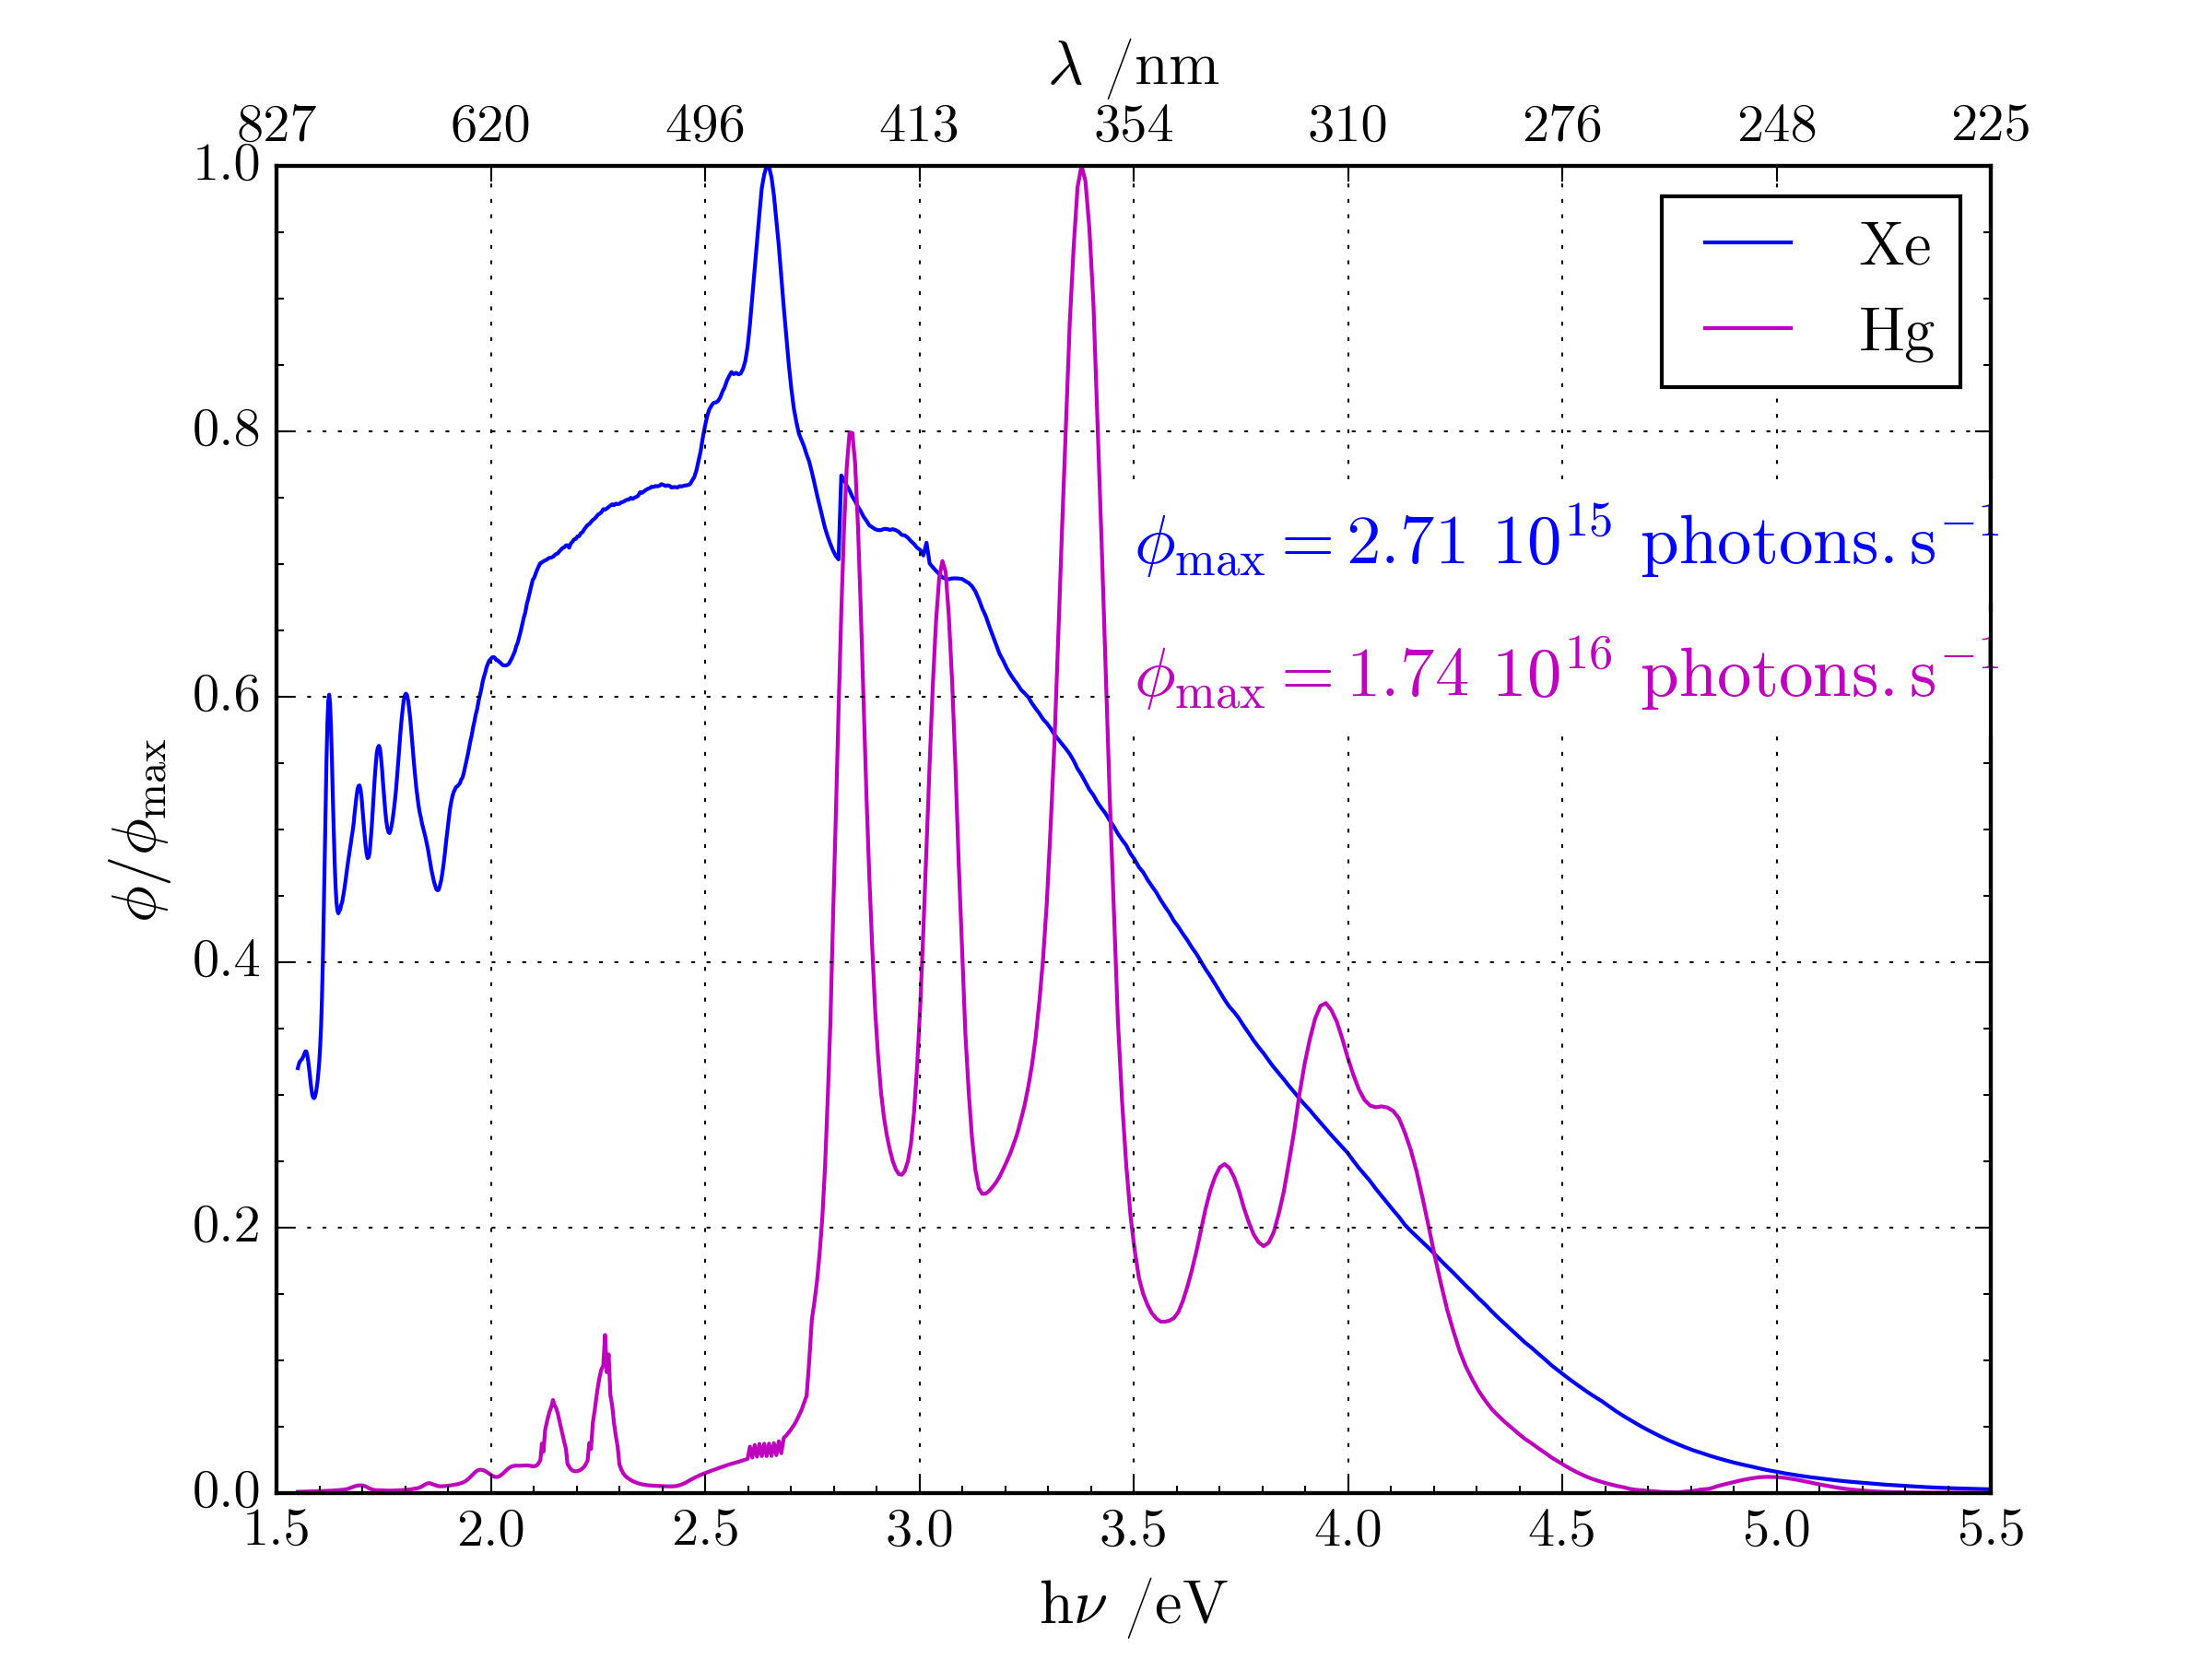
\includegraphics[width=0.65\textwidth]{140834-Illustration-Lamp_Spectra-Relative_Flux.png}
		\caption{Spectres des lampes Xe et Hg normalisés au flux de photon maximum.}
		\label{fig:ch3_lamp_spectra_relative_vs_Hg}
	\end{figure}

    Les caractérisations photoélectrochimiques ont été effectuées avec une source constituée d'une lampe xénon 150W, 
    \emph{Newport 6255}, couplée
    avec un monochromateur à réseaux, \emph{Newport 74125}. 
    Si le flux de photons moyen est environ 10 fois plus faible que celui fourni par la lampe à vapeur de mercure
    (figure \ref{fig:ch3_lamp_spectra_relative_vs_Hg}), le spectre d'émission de la lampe xénon
    est relativement "plat et continu" ce qui permet de minimiser l'erreur sur la monochromaticité réelle lors de son
    passage à travers le monochromateur.

    Dans la suite, la lampe xénon et la lampe à vapeur de mercure seront dénommées \emph{lampe Xe} et \emph{lampe Hg}, respectivement.





\section{Caractérisations photoélectrochimiques}\label{sec:ch3_PEC}

    \subsection{Principe}\label{subsec:ch3_principal_PEC}

    La méthode de caractérisation photoélectrochimique, appelée PEC, utilise les propriétés semiconductrices
    des couches d'oxyde (chapitre \ref{chap:ch1_bib}, \S\ref{sec:state_of_art_PEC}). Elle consiste
    à étudier l'interaction des photons avec le matériau testé. L'illumination d'un semiconducteur de type \emph{n}
    (\emph{p}) en situation d'appauvrissement provoque l'apparition d'un photocourant anodique (cathodique). Pour
    mémoire, la génération du photocourant peut être schématisée par la figure \ref{fig:ch3_photocurrent_generation}.
    

    \begin{figure}[H]
        \centering
        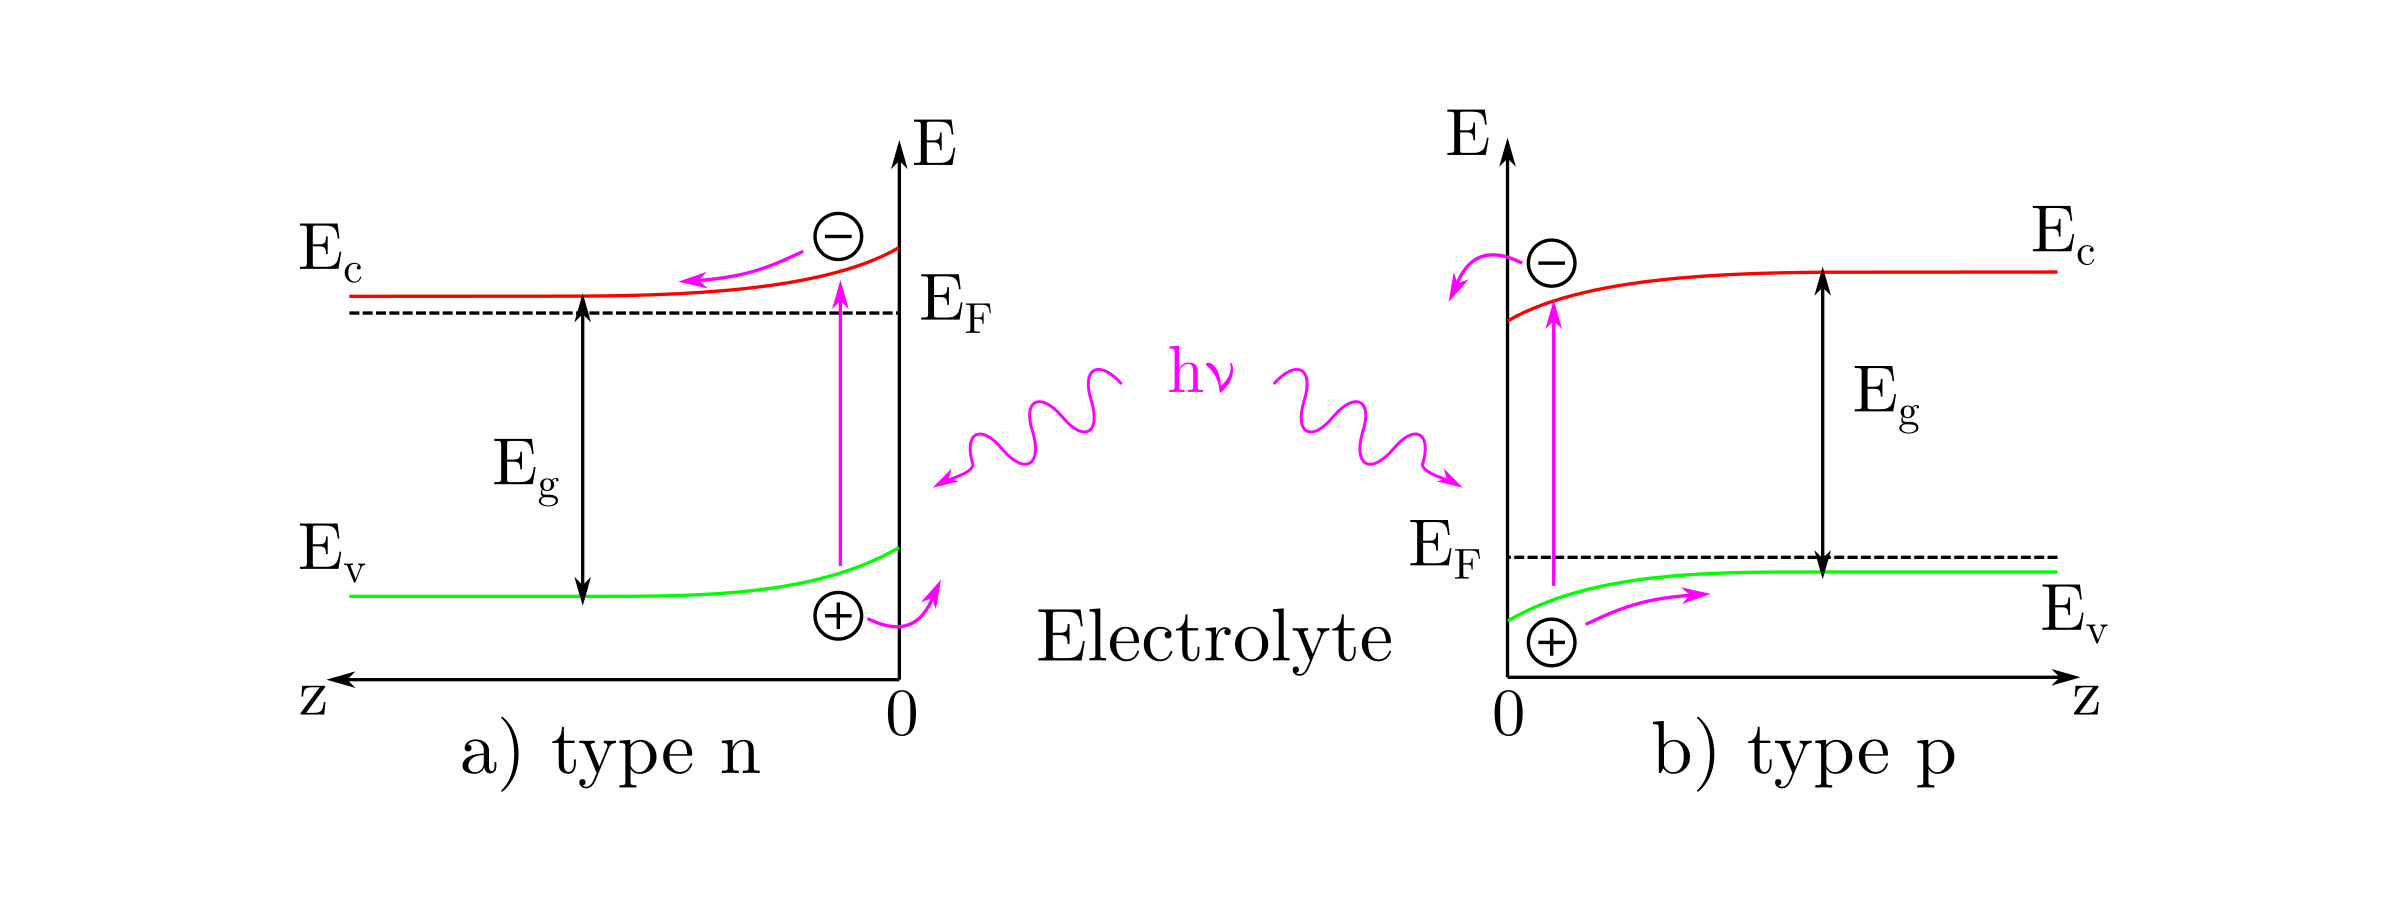
\includegraphics[width=0.85\textwidth]{Photocurrent_Generation.png}
        \caption{Représentation schématique du mécanisme de génération du photocourant.}
       \label{fig:ch3_photocurrent_generation}
    \end{figure}


    Le modèle simplifié de Gärtner-Butler montre que ce photocourant, pour un matériau donné, dépend principalement de deux paramètres: le
    potentiel appliqué et l'énergie des photons incidents. Les deux relations donnant la dépendance du photocourant en
    fonction de l'énergie des photons incidents et du potentiel sont rappelées en équations
    \ref{eq:ch3_iph_linear_transform} et \ref{eq:ch3_iph_linear_transform_potential}.

 
    \begin{equation}
        \left[ \frac{\iph \cdot h\nu}{\phi _0} \right] ^{1/n} = K \cdot (h\nu - \E_g)
        \label{eq:ch3_iph_linear_transform}
    \end{equation}

     \begin{equation}
        \iph^2 = C \cdot (U-U_{fb}-\frac{kT}{e})
        \label{eq:ch3_iph_linear_transform_potential}
    \end{equation}

    \noindent où K est une constante pour un matériau et un potentiel (U) donnés, C une constante pour un
    matériau et une énergie ($h\nu$) donnés, 
    $\iph$ le photocourant mesuré (corrigé du flux de photons $\phi_0$ c'est-à-dire proportionnel au rendement quantique),
    $h\nu$ est l'énergie des photons incidents, $\E _g$ le gap du
    semiconducteur, $U_{fb}$ le potentiel de bandes plates, $U$ le potentiel appliqué, $\phi _0$ le flux de
    photons incidents d'énergie $h\nu$.

    \subsection{Montage et protocole expérimental}\label{subsec:ch3_experimentals}

    Le montage utilisé pour les mesures photoélectrochimiques est un
    montage classique utilisant la technique de détection synchrone ou Lock-in \citep{Stimming1986}. 
    Le dispositif expérimental est présenté de manière schématique sur la figure \ref{fig:ch3_PEC_schematics}.
    La technique consiste à moduler le faisceau lumineux arrivant sur l’électrode de travail à l'aide d'un modulateur,
    dans notre cas un hacheur mécanique \emph{modèle 197} fourni par \emph{Ametek}, 
    dont la fréquence de modulation a été fixée à \SI{15}{\hertz}.
    Le couplage de la lampe xénon 150W au monochromateur permet d’obtenir
    une fenêtre d'énergie de photons de largeur d'environ 3~nm autour d’une valeur moyenne
    ajustable au nanomètre près. Il est possible de réduire la largeur de cette fenêtre en réduisant la largeur des
    fentes d'entrée et de sortie du monochromateur, mais au détriment de l'intensité du flux de photons en sortie du
    monochromateur.

    \begin{figure}[H]
        \centering
        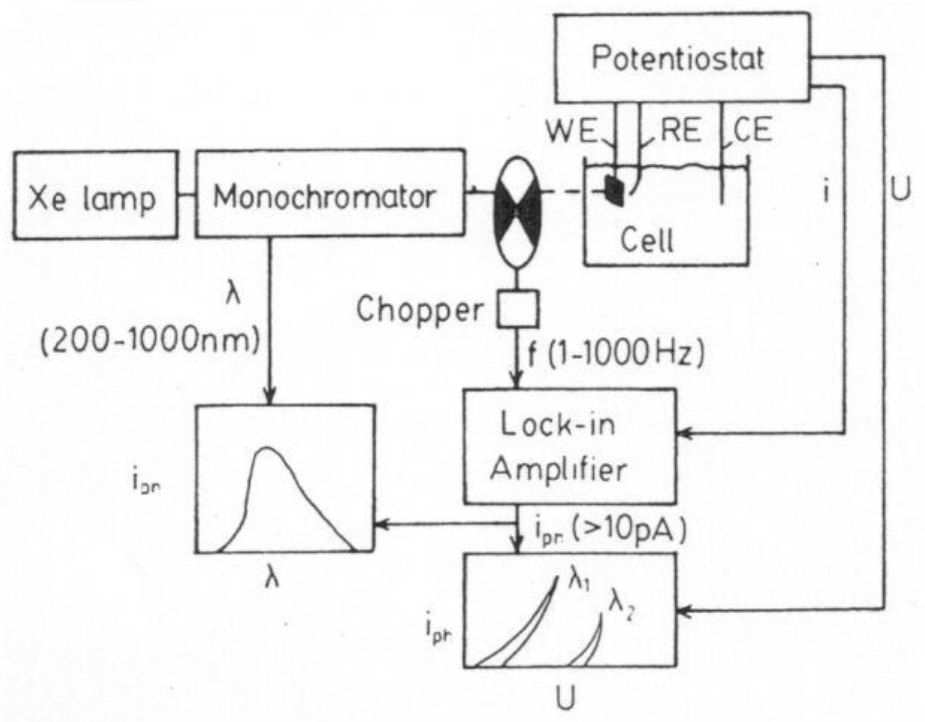
\includegraphics[width=0.65\textwidth]{Stimming_1986_PEC.png}
        \caption[Représentation schématique d'un montage typique de photoélectrochimie.]
        {Représentation schématique du montage de photoélectrochimie (d'après \citet{Stimming1986}).}
       \label{fig:ch3_PEC_schematics}
    \end{figure}

    La modulation de l'intensité du faisceau lumineux illuminant l'échantillon provoque des variations de photocourant 
    à la même fréquence. La mesure de l’amplitude de ces variations et de leur déphasage par rapport
    au signal de référence de modulation délivré par le hacheur, est réalisée par le biais d’une détection
    synchrone \emph{Stanford Research SR830}, dont le signal d’entrée est relié à la sortie courant non
    filtrée du potentiostat \emph{PAR 4000}. Cette procédure permet de séparer le photocourant du bruit et du courant
    électrochimique global même si ces derniers sont très importants et le photocourant faible.

    L'ensemble de l’installation est piloté depuis un ordinateur par le biais d’un
    programme spécifique développé au laboratoire SIMaP. Un "spectre de lampe" est réalisé avant
    chaque série de mesures afin de connaître le flux de photons à chaque énergie arrivant sur l'échantillon.
    Une photodiode silicium calibrée associée à un mesureur de puissance, \emph{Newport 918D-UV-OD3R} est
    utilisé pour cela.

    Afin d'obtenir un photocourant proportionnel au rendement quantique, $\ipht$, le photocourant brut tel que mesuré,
    $\iph$, est corrigé du flux de photons normalisé à sa valeur maximale, $\phi _N$ (équation
    \ref{eq:ch3_Iph_true}). Le photocourant corrigé, $\ipht$, est proportionnel au rendement quantique.

    \begin{equation}
        \ipht (\hv) = \frac{\iph (\hv)}{\phi _N (\hv)}
        \label{eq:ch3_Iph_true}
    \end{equation}
    

    \subsection{Analyse des photocourants}\label{subsec:ch3_interpretation_PEC}

    Dans le but de perturber le moins possible les échantillons testés, la majorité des caractérisations
    photoélectrochimique ont été réalisées au potentiel d'abandon. L'analyse des résultats
    a donc été centrée sur des photocaractéristiques en énergie ou spectres en énergie de photocourant. 
    Deux méthodes d'analyse des résultats étaient disponibles:
    \emph{analyse classique par transformée linéaire} et \emph{analyse avec l'approche recemment développée au SIMaP}
    \citep{Petit2013}.

    \subsubsection{Analyse par transformée linéaire}\label{subsubsec:ch3_linear_transform}
    
    Les photocaractéristiques en énergie peuvent être exploitées en utilisant le modèle simplifié de Gärtner-Butler
    (\S\ref{subsec:ch3_principal_PEC}). Cependant, dans le cas où la réponse en photocourant regroupe les contributions
    de plusieurs phases semiconductrices, ce mode d'analyse ne permet pas d'obtenir de manière précise les paramètres K
    et $\E_g$ des différentes phases.
    
    En effet, la technique employée jusqu'à présent pour décomposer une photocaractéristique en énergie obtenue sur un échantillon,
    constitué de plusieurs phases semiconductrices, consiste à utiliser la transformée linéaire et à linéariser
    la partie basse énergie. L'abscisse à l'origine de cette linéarisation fournit ainsi le gap de la première
    composante.
    La même procédure de linéarisation est effectuée sur la prochaine partie linéaire à plus haute
    énergie. L'intersection entre la première partie linéaire et la seconde est supposée correspondre au gap de la seconde composante.
    La même procédure de linéarisation est répétée jusqu'à ce que toute la plage d'énergie testée ait été traitée
    \citep{Petit2013}. La figure \ref{fig:ch3_linear_transform_PEC} illustre une décomposition de la transformée linéaire
    du photocourant par cette méthode \citep{Petit2013}.

    \begin{figure}[H]
        \centering
        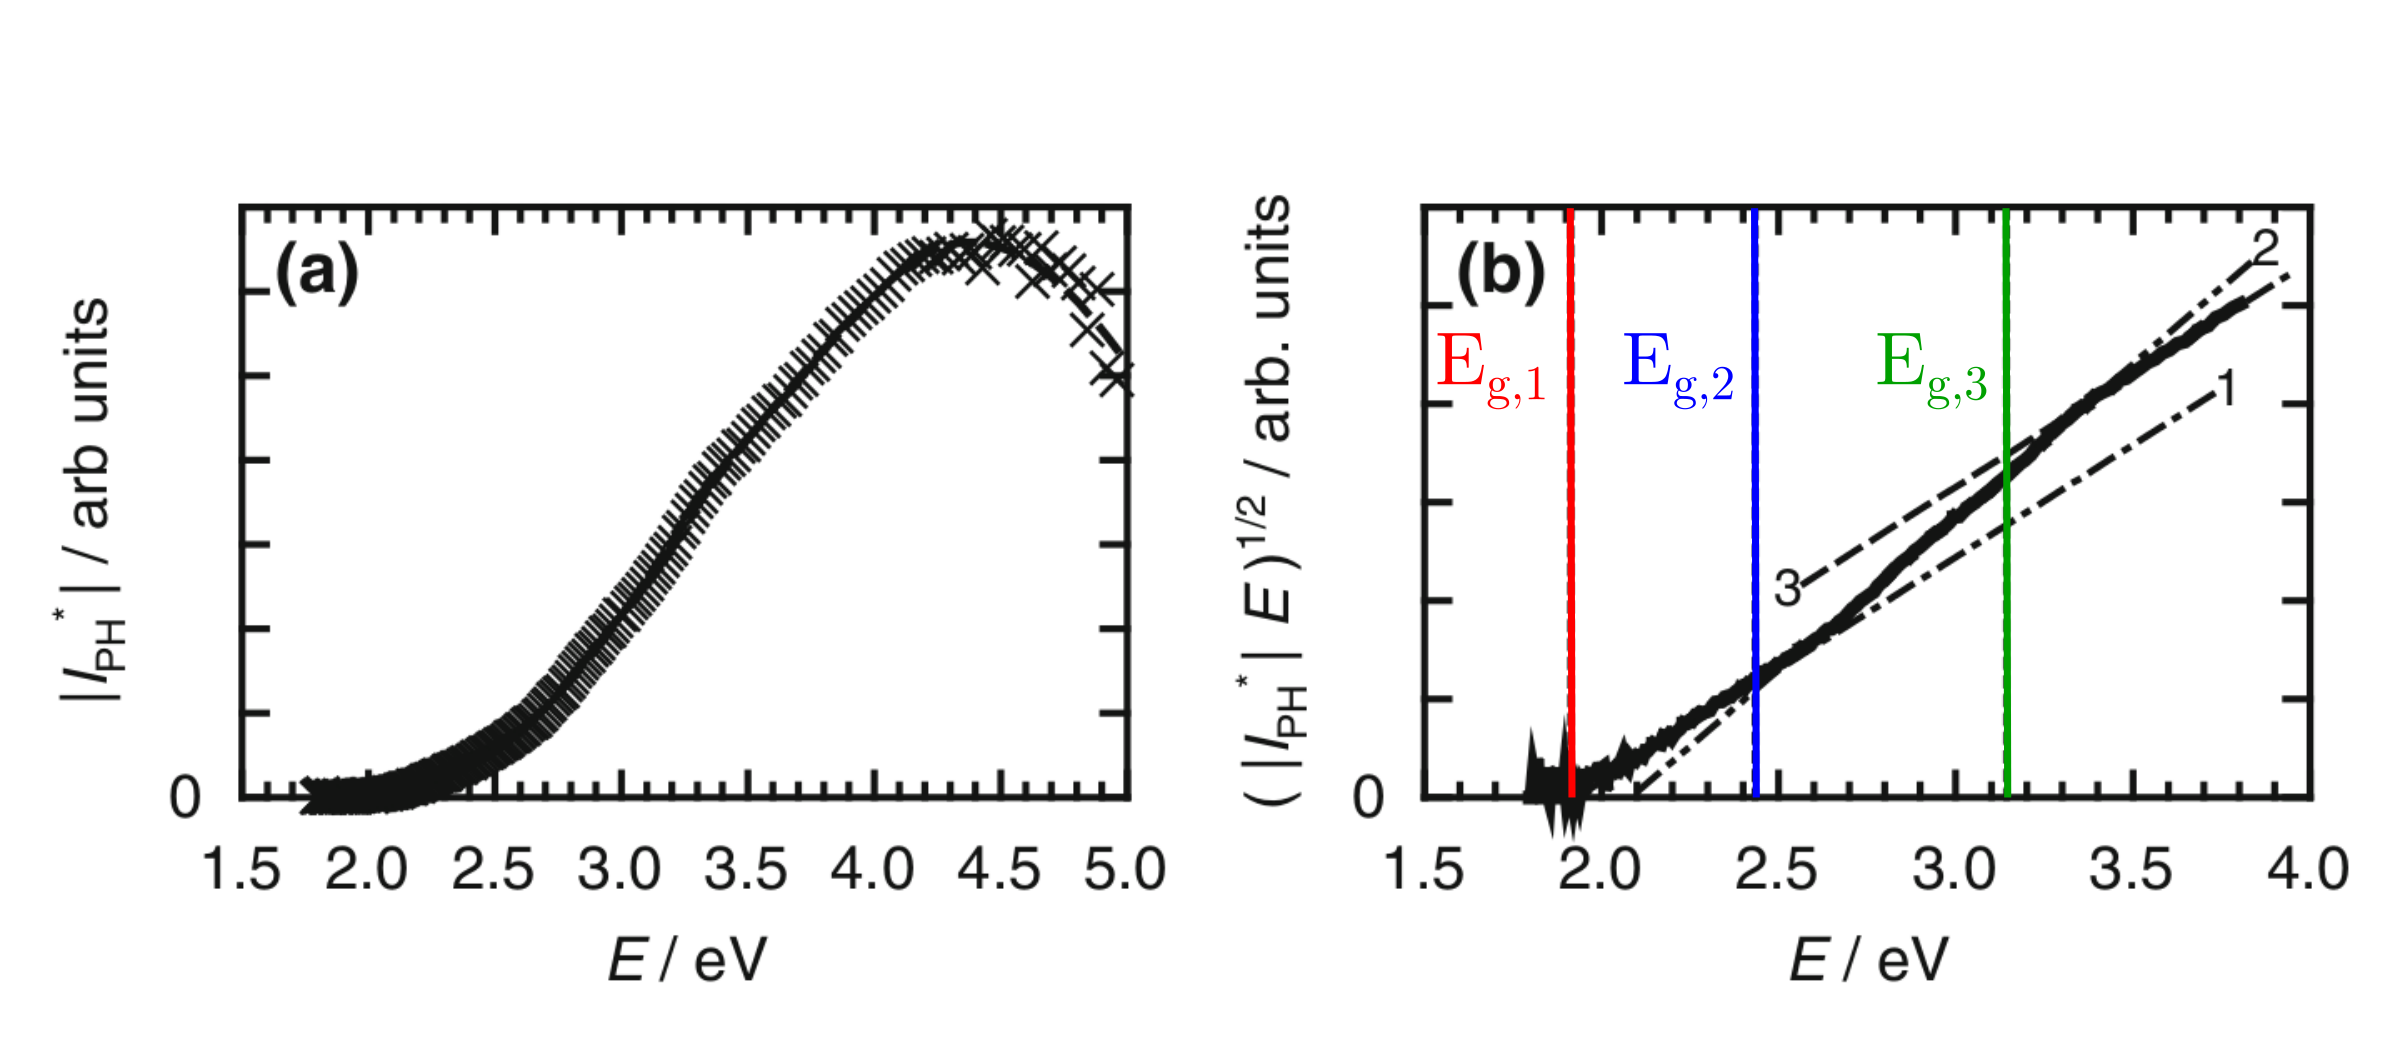
\includegraphics[width=0.90\textwidth]{Linear_Transform_Example.png}
        \caption[Illustration de la méthode classique de décomposition d'une photocaractéristique en énergie avec un échantillon
        multi-constituant:
            a) valeurs expérimentales du module du photocourant $\ipht$,
            b) transformée linéaire de la courbe a).]
        {Illustration de la méthode classique de décomposition d'une photocaractéristique en énergie pour un échantillon
            multi-constituant (d'après \citet{Petit2013}):
        a) valeurs expérimentales du module du photocourant $\ipht$,
        b) transformée linéaire de la courbe a).}
        \label{fig:ch3_linear_transform_PEC}
    \end{figure}
       
    Cette méthode d’analyse devient rapidement laborieuse et imprécise lorsque le nombre
    de phases semiconductrices présentes dans l’échantillon augmente. 
    Jusqu'à présent, cette méthode d'exploitation des photocaractéristiques en énergie fournissait de bons résultats mais
    ne pouvait pas rendre compte de parties linéaires de pentes négatives correspondant à des décroissances de photocourant
    comme par exemple, au-delà de \SI{4.5}{\electronvolt}, sur la figure \ref{fig:ch3_linear_transform_PEC}a).
    Un modèle élaboré au laboratoire  SIMaP par \citet{Petit2013} permet d’expliquer l'allure des photocaractéristiques
    en énergie, et de déterminer les paramètres spécifiques à chaque constituant, d'un échantillon complexe.

    \subsubsection{Analyse avec la nouvelle approche développée au SIMaP}\label{subsubsec:ch3_complex_sum}

    Dans ce modèle, le photocourant $\iph^{\ast}$ est considéré comme un nombre complexe comme l'est l'impédance
    électrochimique. En effet, la modulation de l'illumination implique que le photocourant complexe possède une partie
    réelle $Re \, \iph^{\ast}$ et une partie imaginaire $Im \, \iph^{\ast}$. Le photocourant complexe total, $\iph^{\ast}$, pour un échantillon
    contenant \emph{m} constituants peut alors s'écrire comme la somme des \emph{m} photocourants complexes, $I_{ph,i}^{\ast}$
    selon l'équation \ref{eq:ch3_complex_Iph}. 

    \begin{equation}
        \ipht = \sum _{i=1}^{m} I_{ph,i}^{\ast} = \sum _{i=1}^{m} \vert I_{ph,i}^{\ast} \vert \exp(\mathit{j}\theta _i)
        \label{eq:ch3_complex_Iph}
    \end{equation}

    En considérant que la zone de la charge d'espace est petite devant la profondeur de pénétration de la lumière
    incidente on peut raisonnablement considérer que le taux de recombinaison des paires électrons--trous photogénérées
    ne dépend pas de la longueur d'onde, et donc que le module du photocourant corrigé,
    $\vert I_{ph,i}^{\ast} \vert$, du $\mathit i^{eme}$ constituant suit la forme simplifiée du modèle de
    Gärtner-Butler:     
    
    \begin{equation}
        (\vert I_{ph,i}^{\ast} \vert \cdot h\nu)^{1/n} = K_i (h\nu - \E _{g,i})
        \label{eq:ch3_complex_Iph_modified}
    \end{equation}

    \noindent En combinant les équations
    \ref{eq:ch3_complex_Iph} et \ref{eq:ch3_complex_Iph_modified}, le photocourant complexe total pour \emph{m}
    constituants représentés par \emph{m} triplets ($K_i$, $\theta _i$, $E_{g, i}$) 
    (intensité relative, phase et gap) s'écrit:
    
    \begin{equation}
        \begin{split}
            \ipht &= \sum  _{i=1}^{m} K_i^n \frac{(h\nu - \E _{g,i})^n}{\hv} \exp(\mathit{j}\theta _i) \\
            \iph & = \phi _N \cdot \sum  _{i=1}^{m} K_i^n \frac{(h\nu - \E _{g,i})^n}{\hv} \exp(\mathit{j}\theta _i)
        \end{split}
        \label{eq:ch3_complex_Iph_fully_developped}
    \end{equation}

    Sur la base de ce modèle, il devient possible de déterminer les valeurs des \emph{m} triplets associés aux \emph{m}
    constituants d'un échantillon à partir d'une photocaractéristique en énergie.
    Pour cela, un programme d’ajustement numérique des courbes expérimentales
    a été mis au point au laboratoire SIMaP dans l’environnement Matlab\textregistered .
    Ce programme utilise la procédure fminsearch, basée sur la méthode du
    simplex de \citet{Lagarias1998}, pour trouver le minimum d’une fonction scalaire de plusieurs
    variables non contraintes en partant d’une estimation initiale de ces variables, aléatoires ou non.
    
    Dans cette procédure d’ajustement, un nombre \emph{m} de triplets ($\E_{g,i}$, $K_i$, $\theta _i$) représente le nombre
    supposé de contributions semiconductrices. La fonction scalaire à minimiser, appelée fonction \emph{distance}, 
    est composée du produit de la racine carrée de deux paramètres $\DRe$  et $\DIm$.
    L'équation \ref{eq:ch3_JPP_distance} donne l'expression de la fonction
    \emph{distance} notée D. L'ajustement est réalisé sur les valeurs du photocourant complexe $\ipht$ en
    considérant seulement des transitions indirectes (c'est-à-dire que n est égal à 2). La littérature montre en effet
    que pour des matériaux non parfaits cristallographiquement les transitions sont toujours vues indirectes
    \citep{Stimming1986}.
    
    \begin{equation}
        \begin{split}
            D &= \sqrt{\DRe \cdot \DIm}\\
            D &= \sqrt{ \sum_{h\nu} \left( \ReIphtCalc - \ReIphtExp \right)^2 \cdot \left( \ImIphtCalc - \ImIphtExp
            \right)^2}
        \end{split}
        \label{eq:ch3_JPP_distance}
    \end{equation}


    La valeur de \emph{m} est fixée par l’utilisateur.  
    Ce dernier est libre de choisir, pour les \emph{3m} paramètres, si le paramètre est fixé à
    une valeur définie par l’utilisateur ou si elle est libre d’évoluer lors de la minimisation.
    L’utilisateur doit aussi fournir un jeu de valeurs initiales ou permettre un tirage aléatoire de
    celles-ci. La détermination d’un jeu de valeurs finales stables n’est possible que par
    l’utilisation de plusieurs appels successifs de la procédure de minimisation. Dans ce cas, les
    valeurs finales d’une procédure de minimisation sont utilisées comme valeurs initiales de la
    suivante. 
    
    Pour illustrer ceci, la figure \ref{fig:ch3_table_results_2205} reprend les valeurs
    finales de gaps trouvés, grâce à l’ajustement du spectre de la figure \ref{fig:ch3_linear_transform_PEC},
    fonction de la valeur de \emph{m}. Sur la plage d’énergie de \SI{1.8}{\electronvolt} à
    \SI{4.0}{\electronvolt}, le spectre semble être parfaitement décrit avec trois composantes.
    En effet, le meilleur résultat obtenu avec quatre composantes montre un dédoublement
    de la composante dont le gap est \SI{1.92}{\electronvolt} et celui obtenu pour un ajustement à cinq composantes 
    montre un dédoublement de la composante à \SI{3.11}{\electronvolt} accompagné par une séparation de la composante à
    \SI{1.92}{\electronvolt} en deux composantes ayant des gaps très proches (\SI{1.88}{\electronvolt} et
    \SI{2.06}{\electronvolt}). De même, sur la plage 1.8 à 4.9~eV, le spectre est décrit par quatre composantes, les
    trois identifiées entre 1.8 et 4.0~eV, plus une supplémentaire à 4.07~eV.

     \begin{figure}[H]
        \centering
        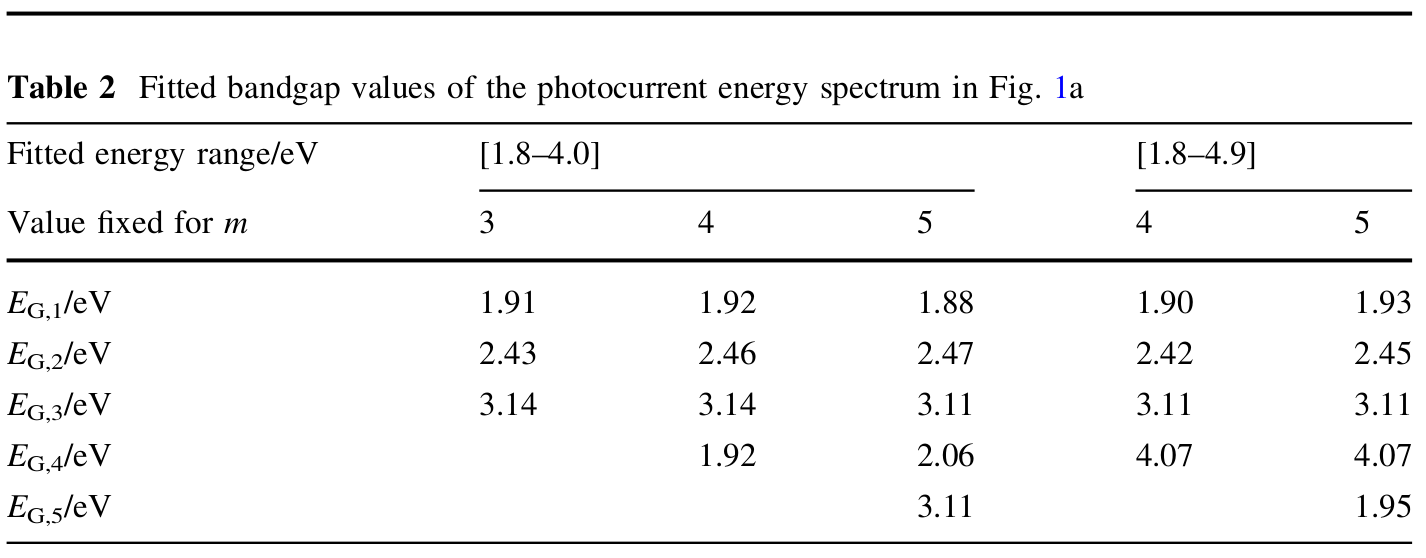
\includegraphics[width=\textwidth]{Petit_2013-Tab2.png}
        \caption[Résultats de l'ajustement de la photocaractéristique en énergie présentée en figure
        \ref{fig:ch3_linear_transform_PEC}a).]
        {Résultats de l'ajustement numérique au modèle du spectre présentée en figure
        \ref{fig:ch3_linear_transform_PEC}a) \citep{Petit2013}.}
        \label{fig:ch3_table_results_2205}
    \end{figure}
    
    Ce modèle a été utilisé avec succès pour analyser des photocaractéristiques en énergie
    mesurées sur des couches d’oxydes formées sur différents alliages \citep{Loucif2012, Srisrual2013, Guillotte2014}.
    Il a permis de montrer qu’une modification de l’allure du spectre en photocourant avec
    le potentiel n’était pas obligatoirement due à l’apparition ou la disparition de phases dans
    la couche d'oxyde, mais pouvait s’expliquer par la modification des réponses de chaque phase
    semiconductrice liée à la modification de leur courbure de bandes.
    
    La figure \ref{fig:ch3_CI_A600_Iph_Ipht} montre
    l'évolution des photocaractéristiques en énergies sur un alliage
    A600 à différents potentiels et le tableau \ref{tab:ch3_fitted_parameters_A600} présente les valeurs des paramètres
    obtenus par ajustement des courbes expérimentales.
    Ces résultats montrent qu’à chacun des potentiels, les valeurs de gaps trouvées sont quasi
    identiques pour les quatre composantes. Chaque photocaractéristique en énergie est donc issue de la réponse de ces
    quatre constituants uniques.

     %\begin{figure}[H]
     %   \centering
     %   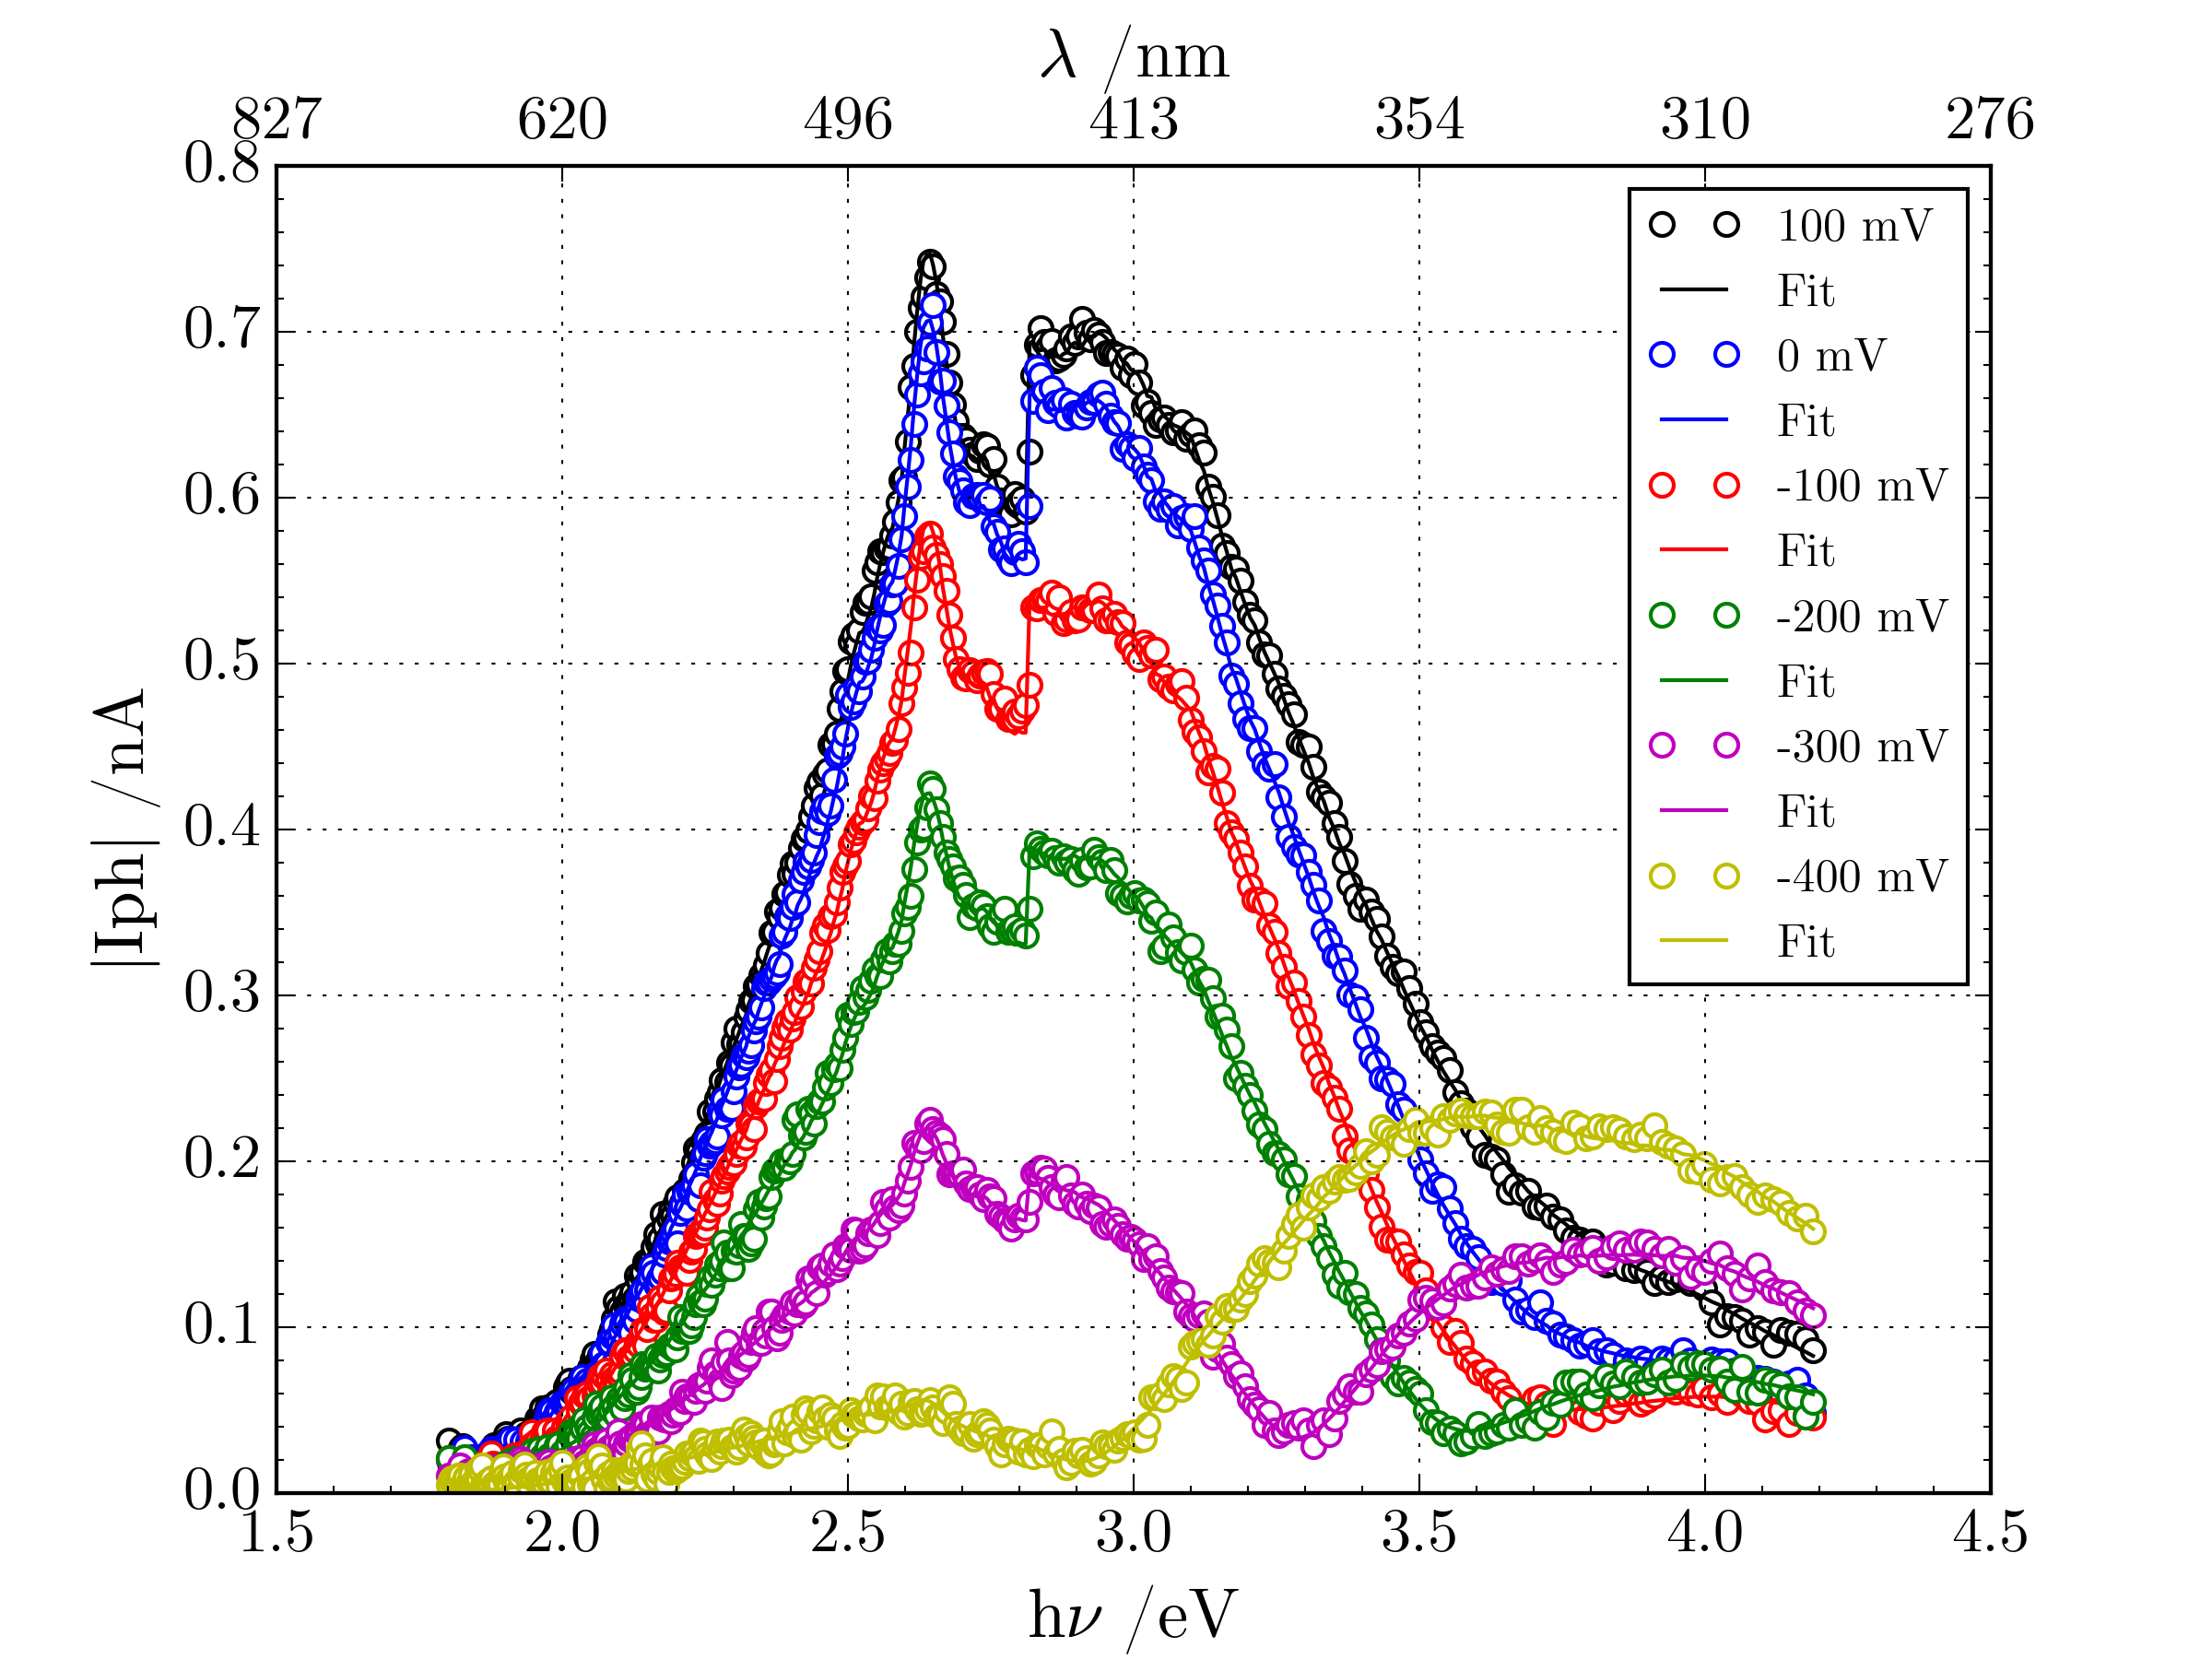
\includegraphics[width=0.85\textwidth]{Abdel-600-All-Iph.png}
     %   \caption[Photocaractéristiques en énergie (photocourant tel que mesuré $\iph$) mesurées à plusieurs potentiels sur l'alliage A600
     %   oxydé thermiquement.]
     %   {Photocaractéristiques en énergie (module du photocourant tel que mesuré $\iph$) mesurées à plusieurs potentiels sur l'alliage A600
     %   oxydé thermiquement d'après \citet{Petit2013}.}
     %   \label{fig:ch3_CI_A600_Iph_Iph}
    %\end{figure}

    \begin{figure}[H]
        \centering
        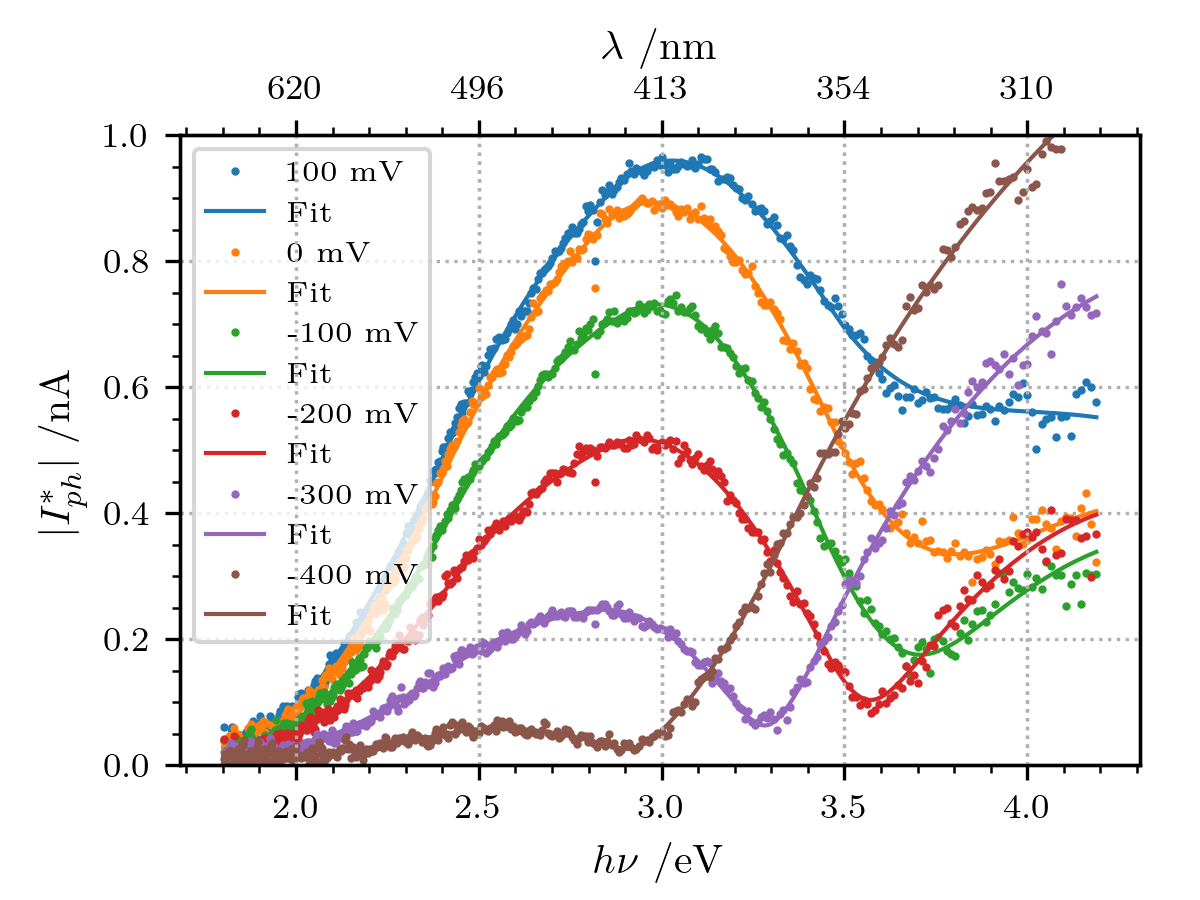
\includegraphics[width=0.85\textwidth]{Abdel-600-All-Ipht.png}
        \caption[Photocaractéristiques en énergie ($\ipht$) mesurées à plusieurs potentiels sur l'alliage A600
        oxydé thermiquement.]
        {Photocaractéristiques en énergie ($\ipht$) mesurées à plusieurs potentiels sur l'alliage A600
        oxydé thermiquement (d'après \citet{Petit2013}).}
        \label{fig:ch3_CI_A600_Iph_Ipht}
    \end{figure}

    \begin{table}[H] 
        \centering
        \begin{footnotesize}
        \rowcolors{3}{lightgray}{}
        \begin{tabular}{l|lll|lll|lll|lll}
        \toprule
            U & $\E_{g,1}$ & $\theta_1$ & $10^{5}K_1$ & $\E_{g,2}$ & $\theta_2$ & $10^{5}K_2$ & $\E_{g,3}$ & $\theta_3$ &
            $10^{5}K_3$ & $\E_{g,4}$ & $\theta_4$ & $10^{5}K_4$\\
            $mV_{MSE}$ & eV & $^{\circ}$ &  & eV & $^{\circ}$ &  & eV & $^{\circ}$ &  & eV & $^{\circ}$ & \\
        \midrule
        100 & 1.75 & -42.8 & 5.2 & 2.43 & 121 & 6.7 & 2.89 & 140 & 6.3 & 3.50 & -60.3 & 9.3 \\\hline
        0 & 1.77 & -49.3 & 5.2 & 2.42 & 119 & 6.3 & 2.82 & 134 & 6.7 & 3.49 & -56.9 & 9.4 \\\hline
        -100 & 1.79 & -52.4 & 4.8 & 2.43 & 120 & 6.1 & 2.88 & 130 & 6.7 & 3.47 & -59.6 & 9.7 \\\hline
        -200 & 1.80 & -53.8 & 4.2 & 2.41 & 120 & 5.3 & 2.84 & 129 & 5.8 & 3.50 & -57.5 & 8.7 \\\hline
        -300 & 1.84 & -52.1 & 3.3 & 2.38 & 124 & 4.3 & 2.79 & 121 & 5.4 & 3.47 & -63.8 & 7.4 \\\hline
        -400 & 1.85 & -48.5 & 1.8 & 2.41 & 121 & 3.7 & 2.85 & 123 & 5.3 & 3.36 & -62.5 & 7.0 \\        
        \bottomrule
        \end{tabular}
        \end{footnotesize}
        \caption[Valeurs des paramètres ajustés pour les photocaractéristiques (figure
        \ref{fig:ch3_CI_A600_Iph_Ipht}).]
        {Valeurs des paramètres ajustés pour les photocaractéristiques en énergie
        de la figure \ref{fig:ch3_CI_A600_Iph_Ipht} d'après \citet{Petit2013} (K en $A^{1/2} eV^{-1/2}$).}
        \label{tab:ch3_fitted_parameters_A600}
    \end{table}

    Néanmoins, l'estimation des intervalles de confiance des paramètres obtenus par ajustement n'est pas implémentée dans la
    procédure décrite précédemment. Dans le cadre de cette thèse, la procédure d'ajustement a été complétée afin de pouvoir estimer
    l'incertitude sur les \emph{3m} paramètres et notamment sur celles des gaps.

   
    \subsubsection{Estimation des intervalles de confiance}\label{subsubsec:ch3_confidence_interval}

    \paragraph{Principes}\mbox{} \\
    Afin de faciliter le développement de la procédure d'ajustement développée par J.P. \textsc{Petit}, cette dernière a
    été réécrite en Python. Python est un langage de programmation interprété et open source très
    largement utilisé dans la communauté scientifique \citep{Langtangen2012, Millman2011, Kiusalaas2010, Oliphant2007}.
    Ce langage possède des librairies optimisées pour le calcul numérique \citep{VanderWalt2011, Jones} avec une
    excellente librairie de visualisation des données \citep{Hunter2007}.

    La fonction distance (eq.\ref{eq:ch3_JPP_distance}), utilisée pour l'ajustement des photocaractéristiques en
    énergie, assure une convergence rapide vers les valeurs optimales des \emph{3m} paramètres définissant les différentes
    contributions semiconductrices. Cependant, elle ne permet pas d'estimer les intervalles de confiance lorsque
    l'optimum est atteint. Pour aller plus loin, nous avons défini une fonction distance alternative calculée pour les
    valeurs optimales des paramètres afin d'estimer les intervalles de confiance. Le traitement statistique des ajustements
    de courbes montre qu'il est possible d'estimer les intervalles de confiance en utilisant la méthode
    des moindres carrés. Cette méthode peut être appliquée à des systèmes non linéaires
    \citep{Bevington2003, Nocedal2006, Press2007}. 
        
    En effet, la méthode des moindres carrés utilise les propriétés de la distribution du $\chi ^2$.
    Par conséquent, cela implique que les mesures expérimentales du photocourant à chaque énergie suivent la loi normale.
    De plus, la méthode des moindres carrés peut être strictement appliquée à condition que les variances expérimentales
    soient connues pour chaque énergie du spectre de photocourant. Cependant, les variances expérimentales ne sont pas
    toujours connues ce qui est le cas pour la caractérisation photoélectrochimique. Dans ce cas de figure, il a été
    nécessaire d'effectuer quelques modifications sur les relations définies dans le cas idéal.

    \subparagraph{Cas idéal} 
    Lorsque les variances $\sigma _{exp}^2$ sont connues, $\chi ^2$ est la fonction distance définie
    dans la méthode des moindres carrés, l'expression en est donnée par l'équation \ref{eq:ch3_chi2}. Les résidus,
    $\epsilon$, pondérés par l'inverse des variances, sont donnée par l'équation \ref{eq:ch3_complex_residuals_X2}.
    $\chi ^2$ peut donc être exprimé comme étant la somme des résidus pondérés comme illustré par l'équation
    \ref{eq:ch3_chi2_vs_eps}. Pour rappel, la variance d'un nombre complexe est un nombre réel positif.
    
    \begin{equation}
        \chi ^2 = \sum _{\hv} \frac{\vert I_{ph,calc} - I_{ph,exp} \vert ^2 }{ \sigma _{exp} ^2}\\
        \label{eq:ch3_chi2}
    \end{equation}

    \begin{equation}
        \epsilon = \frac{\vert I_{ph,calc} - I_{ph,exp} \vert}{\sigma _{exp}}
        \label{eq:ch3_complex_residuals_X2}
    \end{equation}

     \begin{equation}
            \chi ^2 = \sum _{\hv} \epsilon ^2 
        \label{eq:ch3_chi2_vs_eps}
    \end{equation}

    Lorsque les valeurs optimales des paramètres sont atteintes, $\nabla \chi ^2$ tend vers 0.
    La matrice des covariances des paramètres, $\sigma _p^2$, peut être estimée avec le jacobien des
    résidus pondérés, $J_{\epsilon}$. 
    L'expression de la matrice des covariances est donnée par l'équation \ref{eq:ch3_covariance_X2}. 
    Pour des systèmes non linéaires, ce qui est le cas pour le photocourant, l'équation \ref{eq:ch3_covariance_X2} est
    une approximation au premier ordre. En effet, cette approximation est valable car autour de l'optimum les termes du
    second ordre sont très proches de 0 \citep{Press2007}. De plus, cette approximation permet de s'affranchir du calcul
    de l'hessien.

    \begin{equation}
            \sigma _p ^2 = (J_{\epsilon}^T \cdot J_{\epsilon})^{-1} 
        \label{eq:ch3_covariance_X2}
    \end{equation}

    Les termes diagonaux de la matrice des covariance représentent les variances des paramètres.
    L'intervalle de confiance à $\mathcal{P}$~\% des paramètres, notée $CI_{\mathcal{P}}$, est obtenu en multipliant
    les écarts types par le coefficient de student $t_{df,\mathcal{P}}$ avec $df$ étant le nombre de degrés de liberté
    et $\mathcal{P}$ la probabilité de confiance. 
    Le nombre de degrés de liberté correspond au nombre de points en énergie du spectre de
    photocourant, $N$, moins le nombre de paramètres, \emph{3m}.
    La probabilité $\mathcal{P}$ a été fixée à \SI{95}{\percent}.
    L'expression des intervalles de confiance des paramètres est donnée par l'équation \ref{eq:ch3_CI_parameters}.

    \begin{equation}
        \begin{split}
            CI_{\mathcal{P}} &= \sqrt{diag(\sigma _p^2)} \cdot t_{df,\mathcal{P}}\\
            df &= N - 3m\\
            \mathcal{P} &= \SI{95}{\percent}
        \end{split}
        \label{eq:ch3_CI_parameters}
    \end{equation}

    \subparagraph{Cas réel}
    Lorsque les variances expérimentales, $\sigma _{exp}^2$ ne sont pas connues, il est également possible d'estimer
    les intervalles de confiance. Cependant, il est nécessaire d'effectuer quelques modifications sur les relations
    présentées ci-dessus. L'objectif est de définir une fonction distance, S, qui se comporte comme $\chi ^2$ avec un
    facteur constant de mise à l'échelle noté g. La fonction S est définie avec des termes de pondération réels et
    positifs, w, comme illustré par l'équation \ref{eq:ch3_S}.
    De manière similaire à l'équation \ref{eq:ch3_chi2_vs_eps}, la fonction S est définie comme étant la somme résidus
    pondérés $\epsilon ^{\prime}$.

    \begin{equation}
       \begin{split} 
            S &= \sum _{\hv} \vert I_{ph,calc} - I_{ph,exp}\vert ^2 \cdot w \\
            \epsilon ^{\prime} &=  \vert I_{ph,calc} - I_{ph,exp} \vert \cdot \sqrt{w}\\
            S &= \sum _{\hv} \epsilon ^{\prime 2} 
       \end{split}     
       \label{eq:ch3_S}
    \end{equation}

    Les termes de pondération sont définis de manière à faire apparaître le facteur constant de mise à l'échelle
    ainsi que les variances expérimentales dont l'expression est donnée par l'équation \ref{eq:ch3_w}. 
    Cela revient à considérer une relation de proportionnalité entre les termes de pondération et les variances.

    \begin{equation}
            w = g \cdot \frac{1}{\sigma _{exp} ^2}
            \label{eq:ch3_w}
    \end{equation}

    En remplaçant w dans l'équation \ref{eq:ch3_S} par l'expression de l'équation \ref{eq:ch3_w}, une relation de
    proportionnalité apparaît entre S et $\chi^2$. 
    De plus, $\chi^2/\nu$ tend vers 1 lorsque les valeurs optimales des paramètres sont déterminées.
    Par conséquent, le facteur de mise à l'échelle, g, peut être facilement
    calculé avec la valeur optimale de S comme le montre l'équation \ref{eq:ch3_S_vs_X2}. 

    \begin{equation}
        \begin{split}
            S &= g \cdot \chi ^2 \\
            \frac{S}{\nu} &= g \cdot \frac{\chi^2}{\nu} \approx g\\
        \end{split}
        \label{eq:ch3_S_vs_X2}
    \end{equation}

    Grâce au facteur de mise à l'échelle, g, la matrice des covariances des paramètres, $\sigma _p$, peut être estimée avec le jacobien des
    résidus pondérés, $J_{\epsilon ^{\prime}}$. L'expression de la matrice des covariances est donnée par l'équation
    \ref{eq:ch3_covariance_S}. Les intervalles de confiance des paramètres sont calculées en reprenant l'expression de
    l'équation \ref{eq:ch3_CI_parameters}.    
    
    \begin{equation}
        \begin{split}
            \sigma _p ^{\prime 2} &= (J_{\epsilon^{\prime}}^T \cdot J_{\epsilon^{\prime}})^{-1} \\
            \sigma _p ^2 &= g \cdot \sigma _p ^{\prime 2}
        \end{split}    
        \label{eq:ch3_covariance_S}
    \end{equation}

    Le choix des termes de pondération a été fait en considérant que la variance $\sigma _{exp}^2$ est proportionnelle
    au bruit moyen, $\overline{\epsilon}_d$, sur le module du "photocourant" mesuré au noir c'est-à-dire sans illumination. De plus, il a été
    supposé que la variance est d'autant plus petite que le rendement quantique est grand. Ce dernier est représenté, à une
    constante prêt, par le module du photocourant corrigé du flux de photon et normalisé à sa valeur
    maximale noté $\vert I_{ph_N}^{\ast} \vert$.     
    La normalisation assure que les termes de pondérations ont la même dimension que l'inverse des
    variances comme illustré par l'équation \ref{eq:ch3_weights}. De cette manière, S est adimensionelle tout comme $\chi ^2$.
    Le jacobien, $J_{\epsilon ^{\prime}}$, est estimé numériquement en fixant le pas de la différence finie à la racine
    carrée de la précision de la machine \citep{Nocedal2006, Press2007}. 

    \begin{equation}
        \begin{split}
            \sigma _{exp} & \propto \frac{\overline{\epsilon}_d}{\vert I_{ph_N}^{\ast} \vert }\\
            w &= \frac{1}{\sigma _{exp}^2} = g \cdot \frac{\vert I_{ph_N}^{\ast} \vert ^2}{\overline{\epsilon}_d^2}
        \end{split}    
        \label{eq:ch3_weights}
    \end{equation}

    \paragraph{Applications}\mbox{}\\
    Les termes de pondération tels qu'ils viennent d'être définis reflètent le ratio signal/bruit. Dans un premier temps,
    afin de tester la pertinence de notre
    choix des termes de pondération, des photocaractéristiques en énergie ont été recalculées 
    (equations \ref{eq:ch3_complex_Iph_fully_developped}) à partir des valeurs de paramètres obtenus par
    \citet{Petit2013}, indiquées dans le tableau \ref{tab:ch3_initial_values_noise}.
    
    \begin{table}[H]
        \centering
        \begin{tabular}{p{0.3\textwidth}|%
                        p{0.18\textwidth}%
                        p{0.18\textwidth}%
                        p{0.18\textwidth}}
            \toprule
            & $10^5K_i$ & $\theta _i$ & $\E_{g,i}$ \\ 
            & $A^{1/2} eV^{1/2}$ & $^{\circ}$ & eV \\ \midrule
            Valeurs intiales & $4.6$ & $7$ & $1.91$ \\
            des paramètres & $5.4$ & $-33$ & $2.44$ \\
            & $7$ & $156$ & $3.16$\\  
            \bottomrule
        \end{tabular}  
        \caption[Valeurs de paramètres obtenus par ajustement numérique de la figure
        \ref{fig:ch3_linear_transform_PEC}a).]
        {Valeurs de paramètres obtenus par \citet{Petit2013} par ajustement numérique de la figure
        \ref{fig:ch3_linear_transform_PEC}a).}
        \label{tab:ch3_initial_values_noise}
    \end{table}    

    Aux valeurs calculées de $\iph$ a été ajouté un bruit de plus en plus élevé. 
    Le bruit a été calculé en utilisant la loi normale centrée $\mathcal{N}(0, \sigma)$ où
    $\sigma$ a été fixée à la valeur minimale du module du photocourant calculé, et qui a été amplifiée avec un
    facteur d'amplification $f_a$. Le bruit ainsi généré est ajouté aux parties réelle et imaginaire du photocourant
    $\iph$.    
    Les modules du
    photocourant $\ipht$ pour différents facteurs d'amplification du bruit sont représentés sur la figure
    \ref{fig:ch3_noise_test}, et les valeurs de paramètres correspondantes issues des ajustements des courbes ainsi
    obtenues sont données dans le tableau
    \ref{tab:ch3_fitted_parameters_noise_test}.
    La largeur des intervalles de confiance pour ces paramètres augmente bien avec la diminution du
    ratio signal/bruit comme attendu. 

     \begin{table}[H] 
        \centering
        \begin{tabular}{p{0.3\textwidth}|%
                        p{0.18\textwidth}%
                        p{0.18\textwidth}%
                        p{0.18\textwidth}}
            \toprule
            Facteur d'amplification & $10^5K_i$ & $\theta _i$ & $\E_{g,i}$ \\ 
            du bruit $f_a$                & $A^{1/2} eV^{1/2}$ & $^{\circ}$ & eV \\ \midrule
             \rowcolor{lightgray}& $4.6000 \pm 0.0002$ & $7.00 \pm 0.02$ & $1.9100 \pm 0.0002$ \\
             \rowcolor{lightgray}& $5.4000 \pm 0.0004$ & $-33.00 \pm 0.02$ & $2.4400 \pm 0.0003$ \\
            \rowcolor{lightgray}\multirow{-3}{*}{0.001} & $7.0005 \pm 0.0009$ & $156.00 \pm 0.02$ & $3.1600 \pm 0.0009$ \\ \hline
             & $4.6 \pm 0.2$ & $7 \pm 4$ & $1.91 \pm 0.04$ \\
             & $5.5 \pm 0.4$ & $-33 \pm 5$ & $2.45 \pm 0.08$ \\
            \multirow{-3}{*}{1} & $7.0 \pm 0.3$ & $156 \pm 4$ & $3.15 \pm 0.04$ \\ \hline
             \rowcolor{lightgray}& $4.6 \pm 0.6$ & $7 \pm 7$ & $1.91 \pm 0.09$ \\
             \rowcolor{lightgray}& $5.5 \pm 0.7$ & $-32 \pm 20$ & $2.4 \pm 0.2$ \\
             \rowcolor{lightgray}\multirow{-3}{*}{2}& $7.0 \pm 0.5$ & $160 \pm 6$ & $3.18 \pm 0.07$ \\ \hline
             & $5 \pm 3$ & $8 \pm 30$ & $1.9 \pm 0.4$ \\
             & $5 \pm 3$ & $-38 \pm 50$ & $2.4 \pm 0.5$ \\
             \multirow{-3}{*}{5}& $7 \pm 3$ & $154 \pm 20$ & $3.2 \pm 0.2$ \\ \hline
             \rowcolor{lightgray}& $5 \pm 8$ & $10 \pm 80$ & $1.9 \pm 0.9$ \\
             \rowcolor{lightgray}& $5 \pm 6$ & $-43 \pm 200$ & $2 \pm 2$ \\
             \rowcolor{lightgray}\multirow{-3}{*}{10}& $6 \pm 4$ & $155 \pm 60$ & $3.1 \pm 0.7$ \\ 
        \bottomrule
        \end{tabular}
        \caption{Valeurs des paramètres obtenus par ajustement des photocaractéristiques en énergie avec différents facteurs
        d'amplification du bruit ($f_a$).}
        \label{tab:ch3_fitted_parameters_noise_test}
    \end{table}


     \begin{figure}[H]
        \centering
        \begin{subfigure}[b]{0.48\textwidth}
            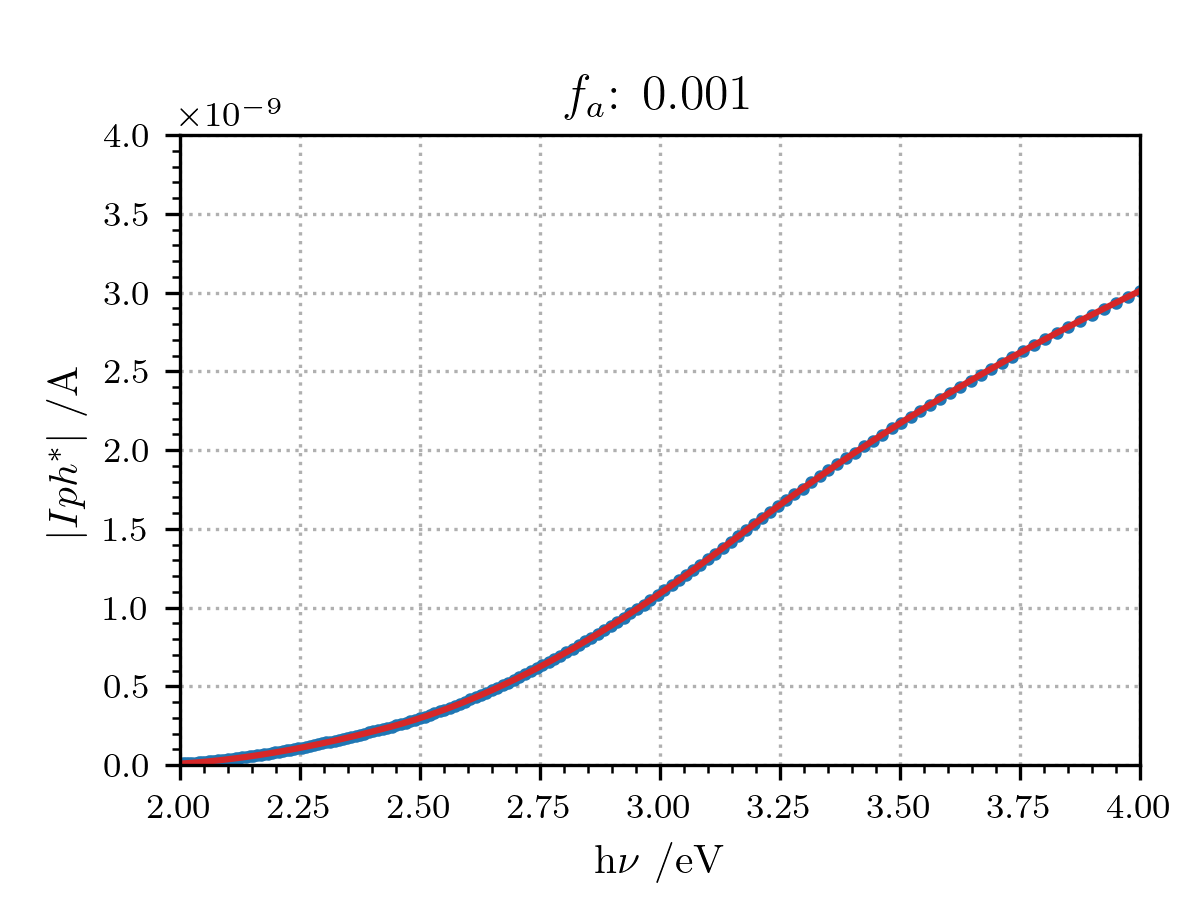
\includegraphics[width=\textwidth]{DSS_0mV_data-Iph-0001x.png}
            \caption{}
            \label{}
        \end{subfigure}
        \begin{subfigure}[b]{0.48\textwidth}
            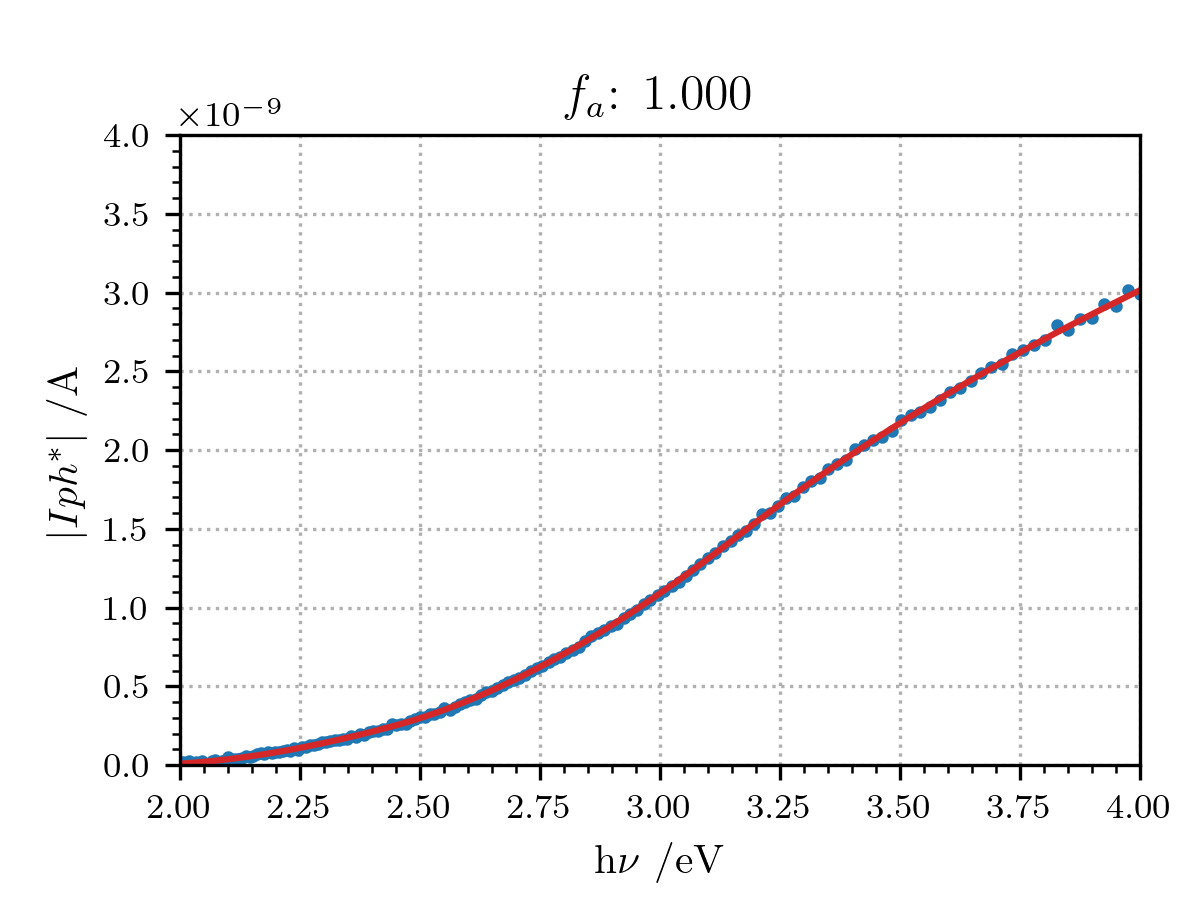
\includegraphics[width=\textwidth]{DSS_0mV_data-Iph-1x.png}
            \caption{}
            \label{}
        \end{subfigure}
        \begin{subfigure}[b]{0.48\textwidth}
            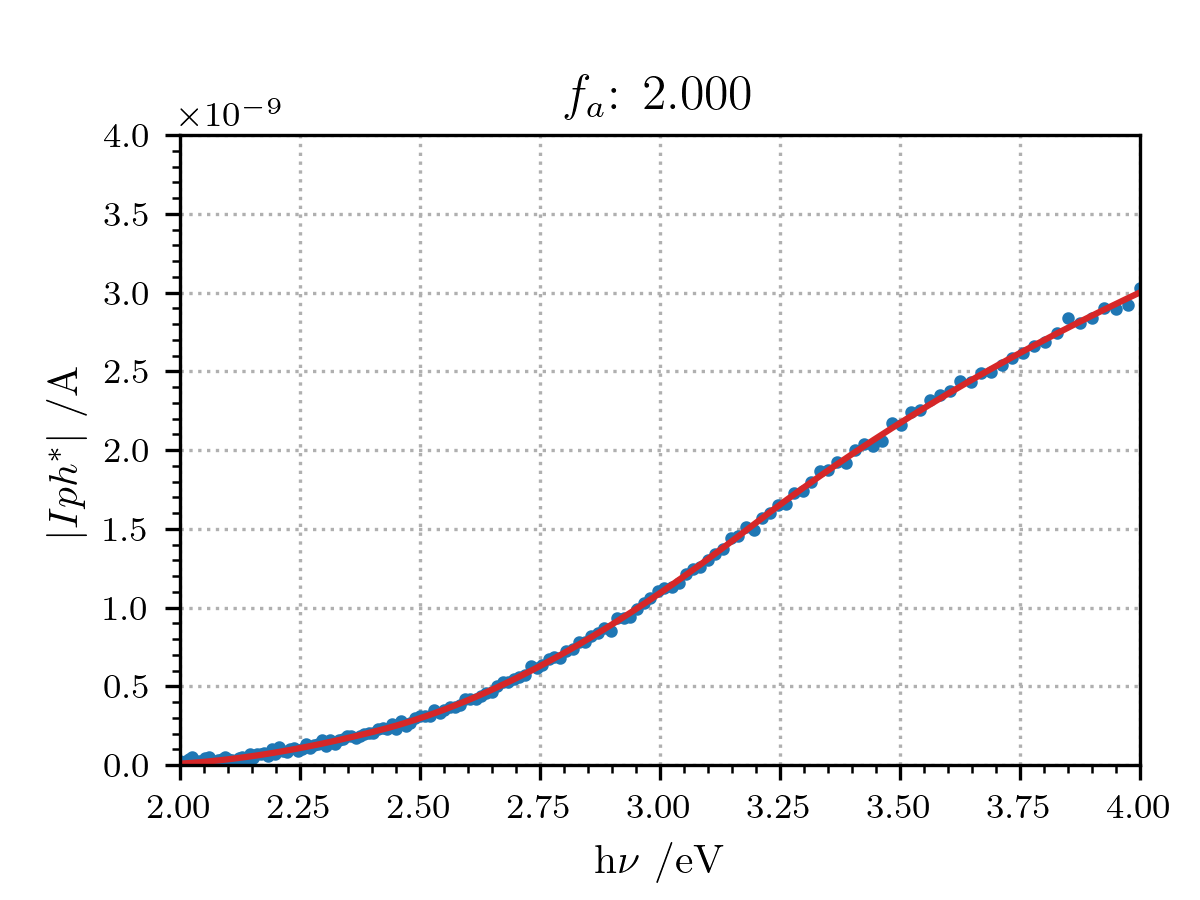
\includegraphics[width=\textwidth]{DSS_0mV_data-Iph-2x.png}
            \caption{}
            \label{}
        \end{subfigure}
    \end{figure}
    \begin{figure}[H]
        \ContinuedFloat
        \begin{subfigure}[b]{0.48\textwidth}
            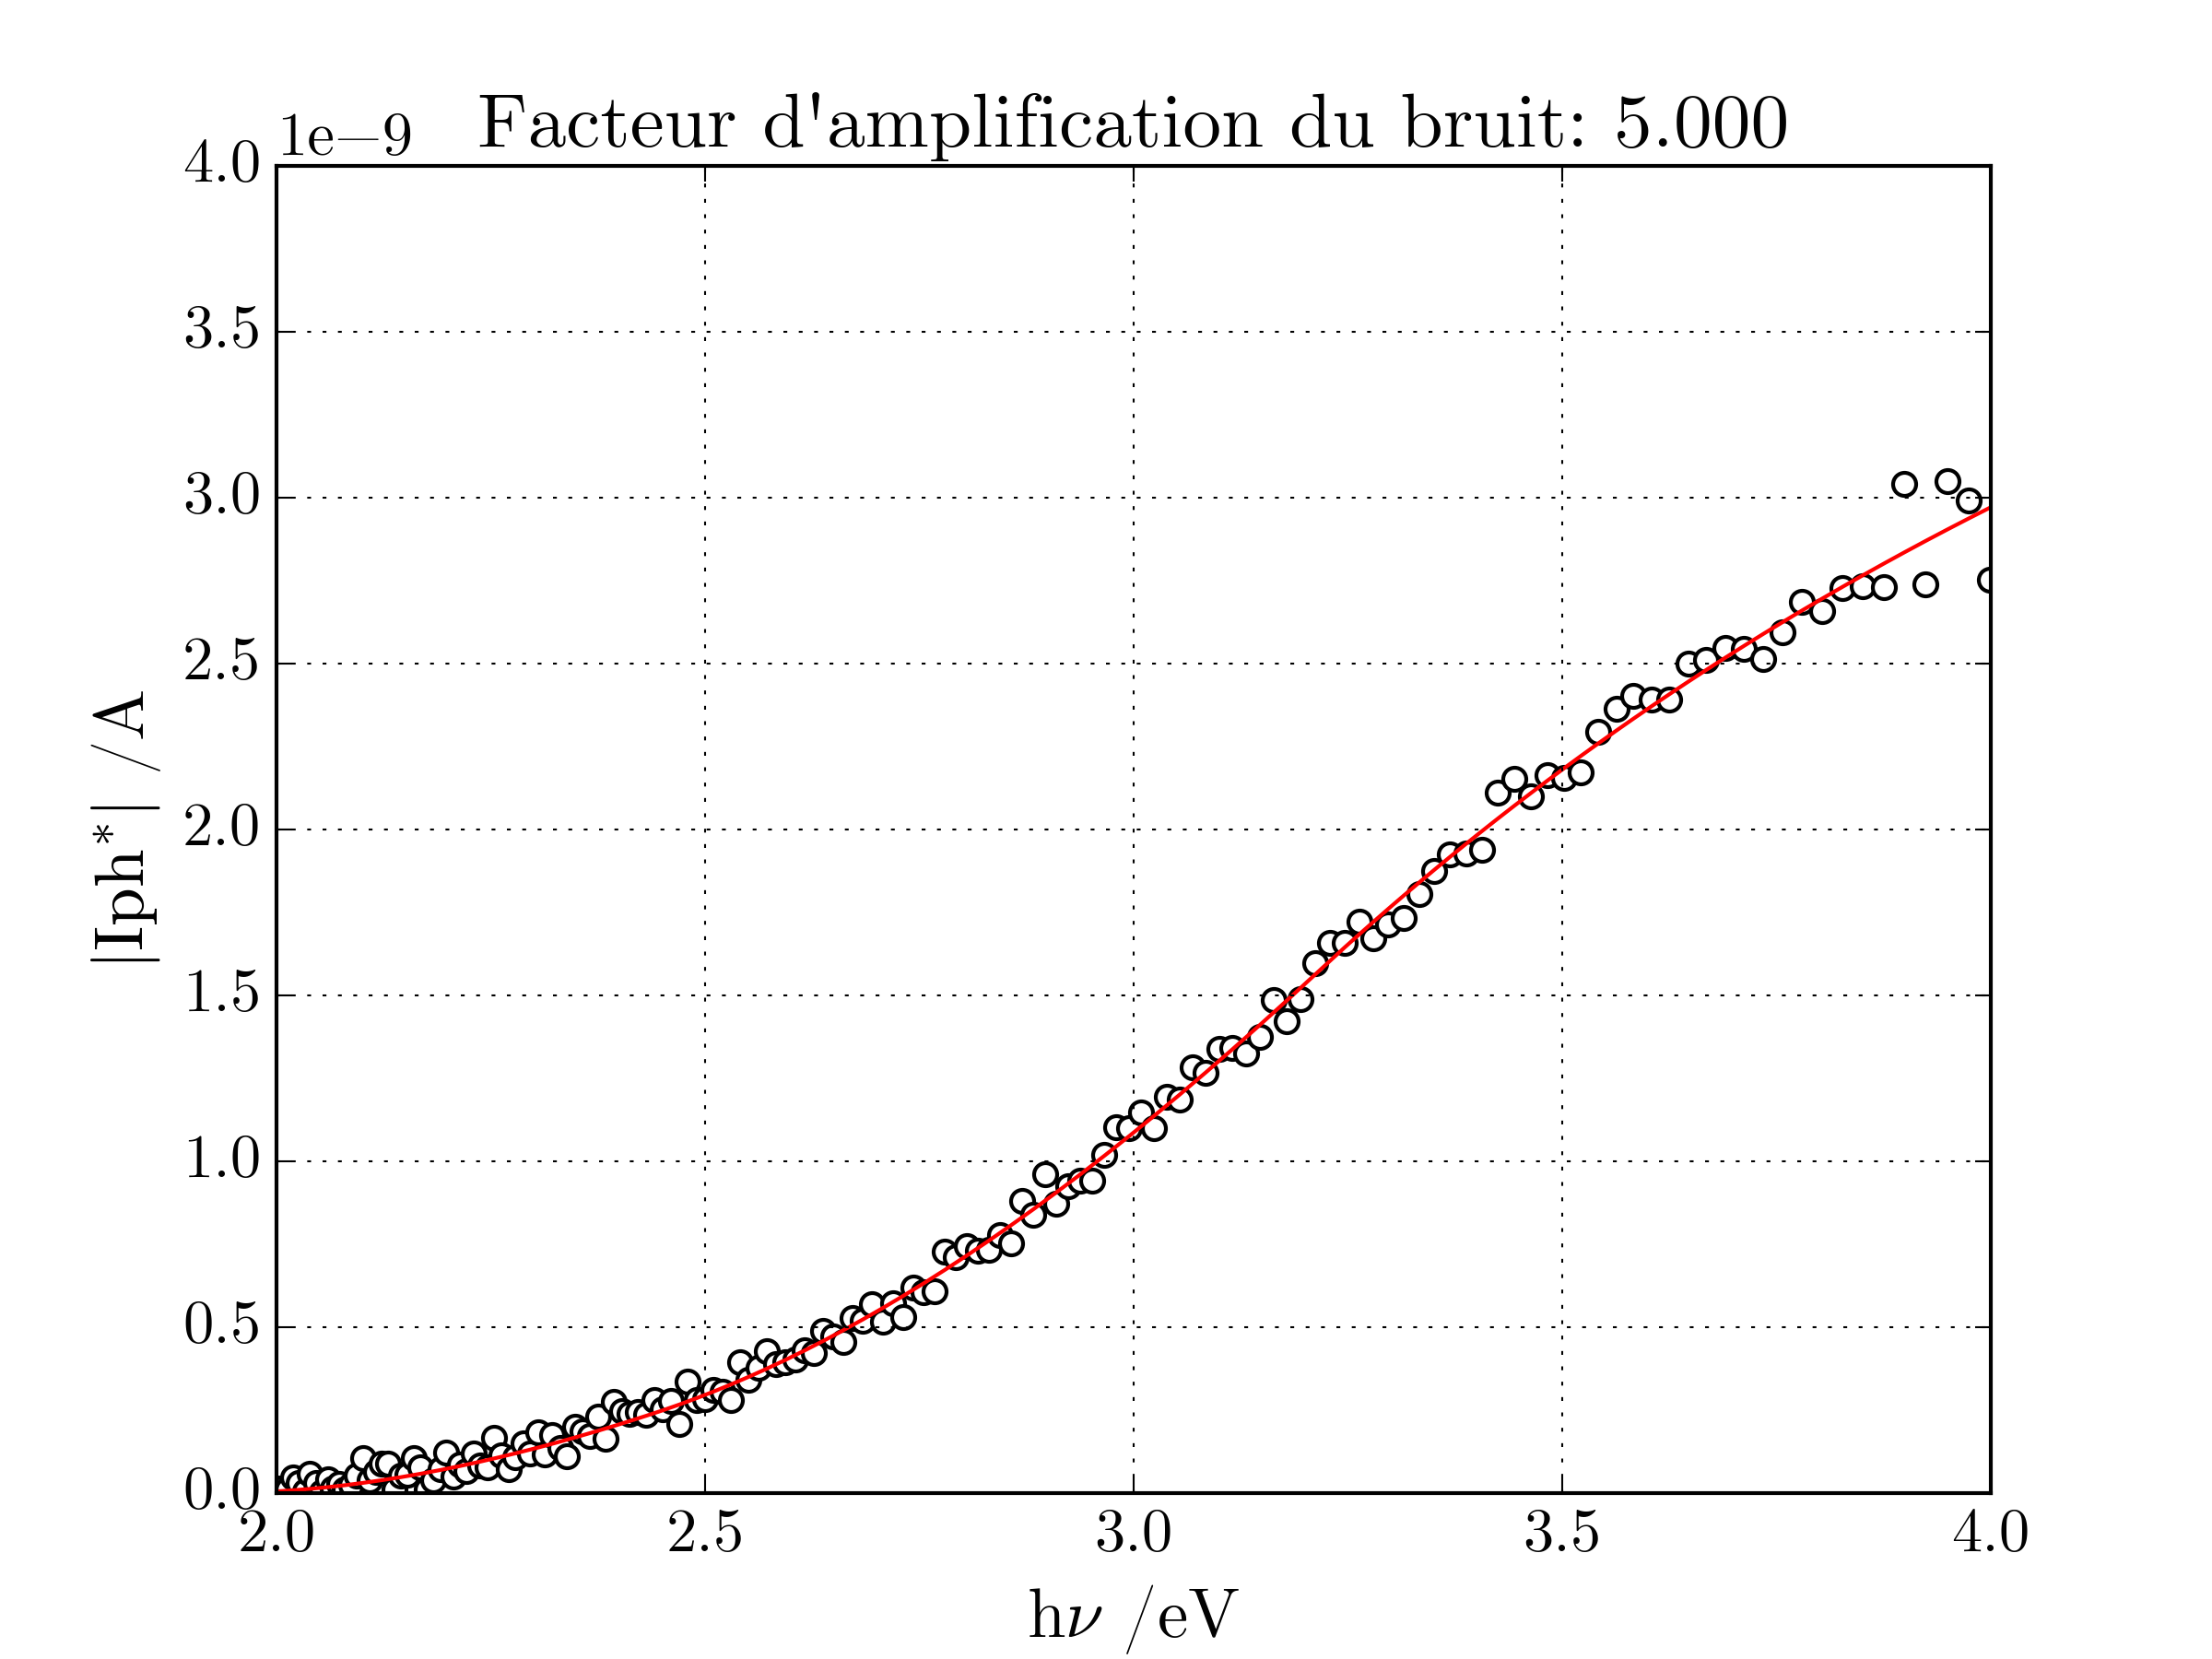
\includegraphics[width=\textwidth]{DSS_0mV_data-Iph-5x.png}
            \caption{}
            \label{}
        \end{subfigure}
        \begin{subfigure}[b]{0.48\textwidth}
            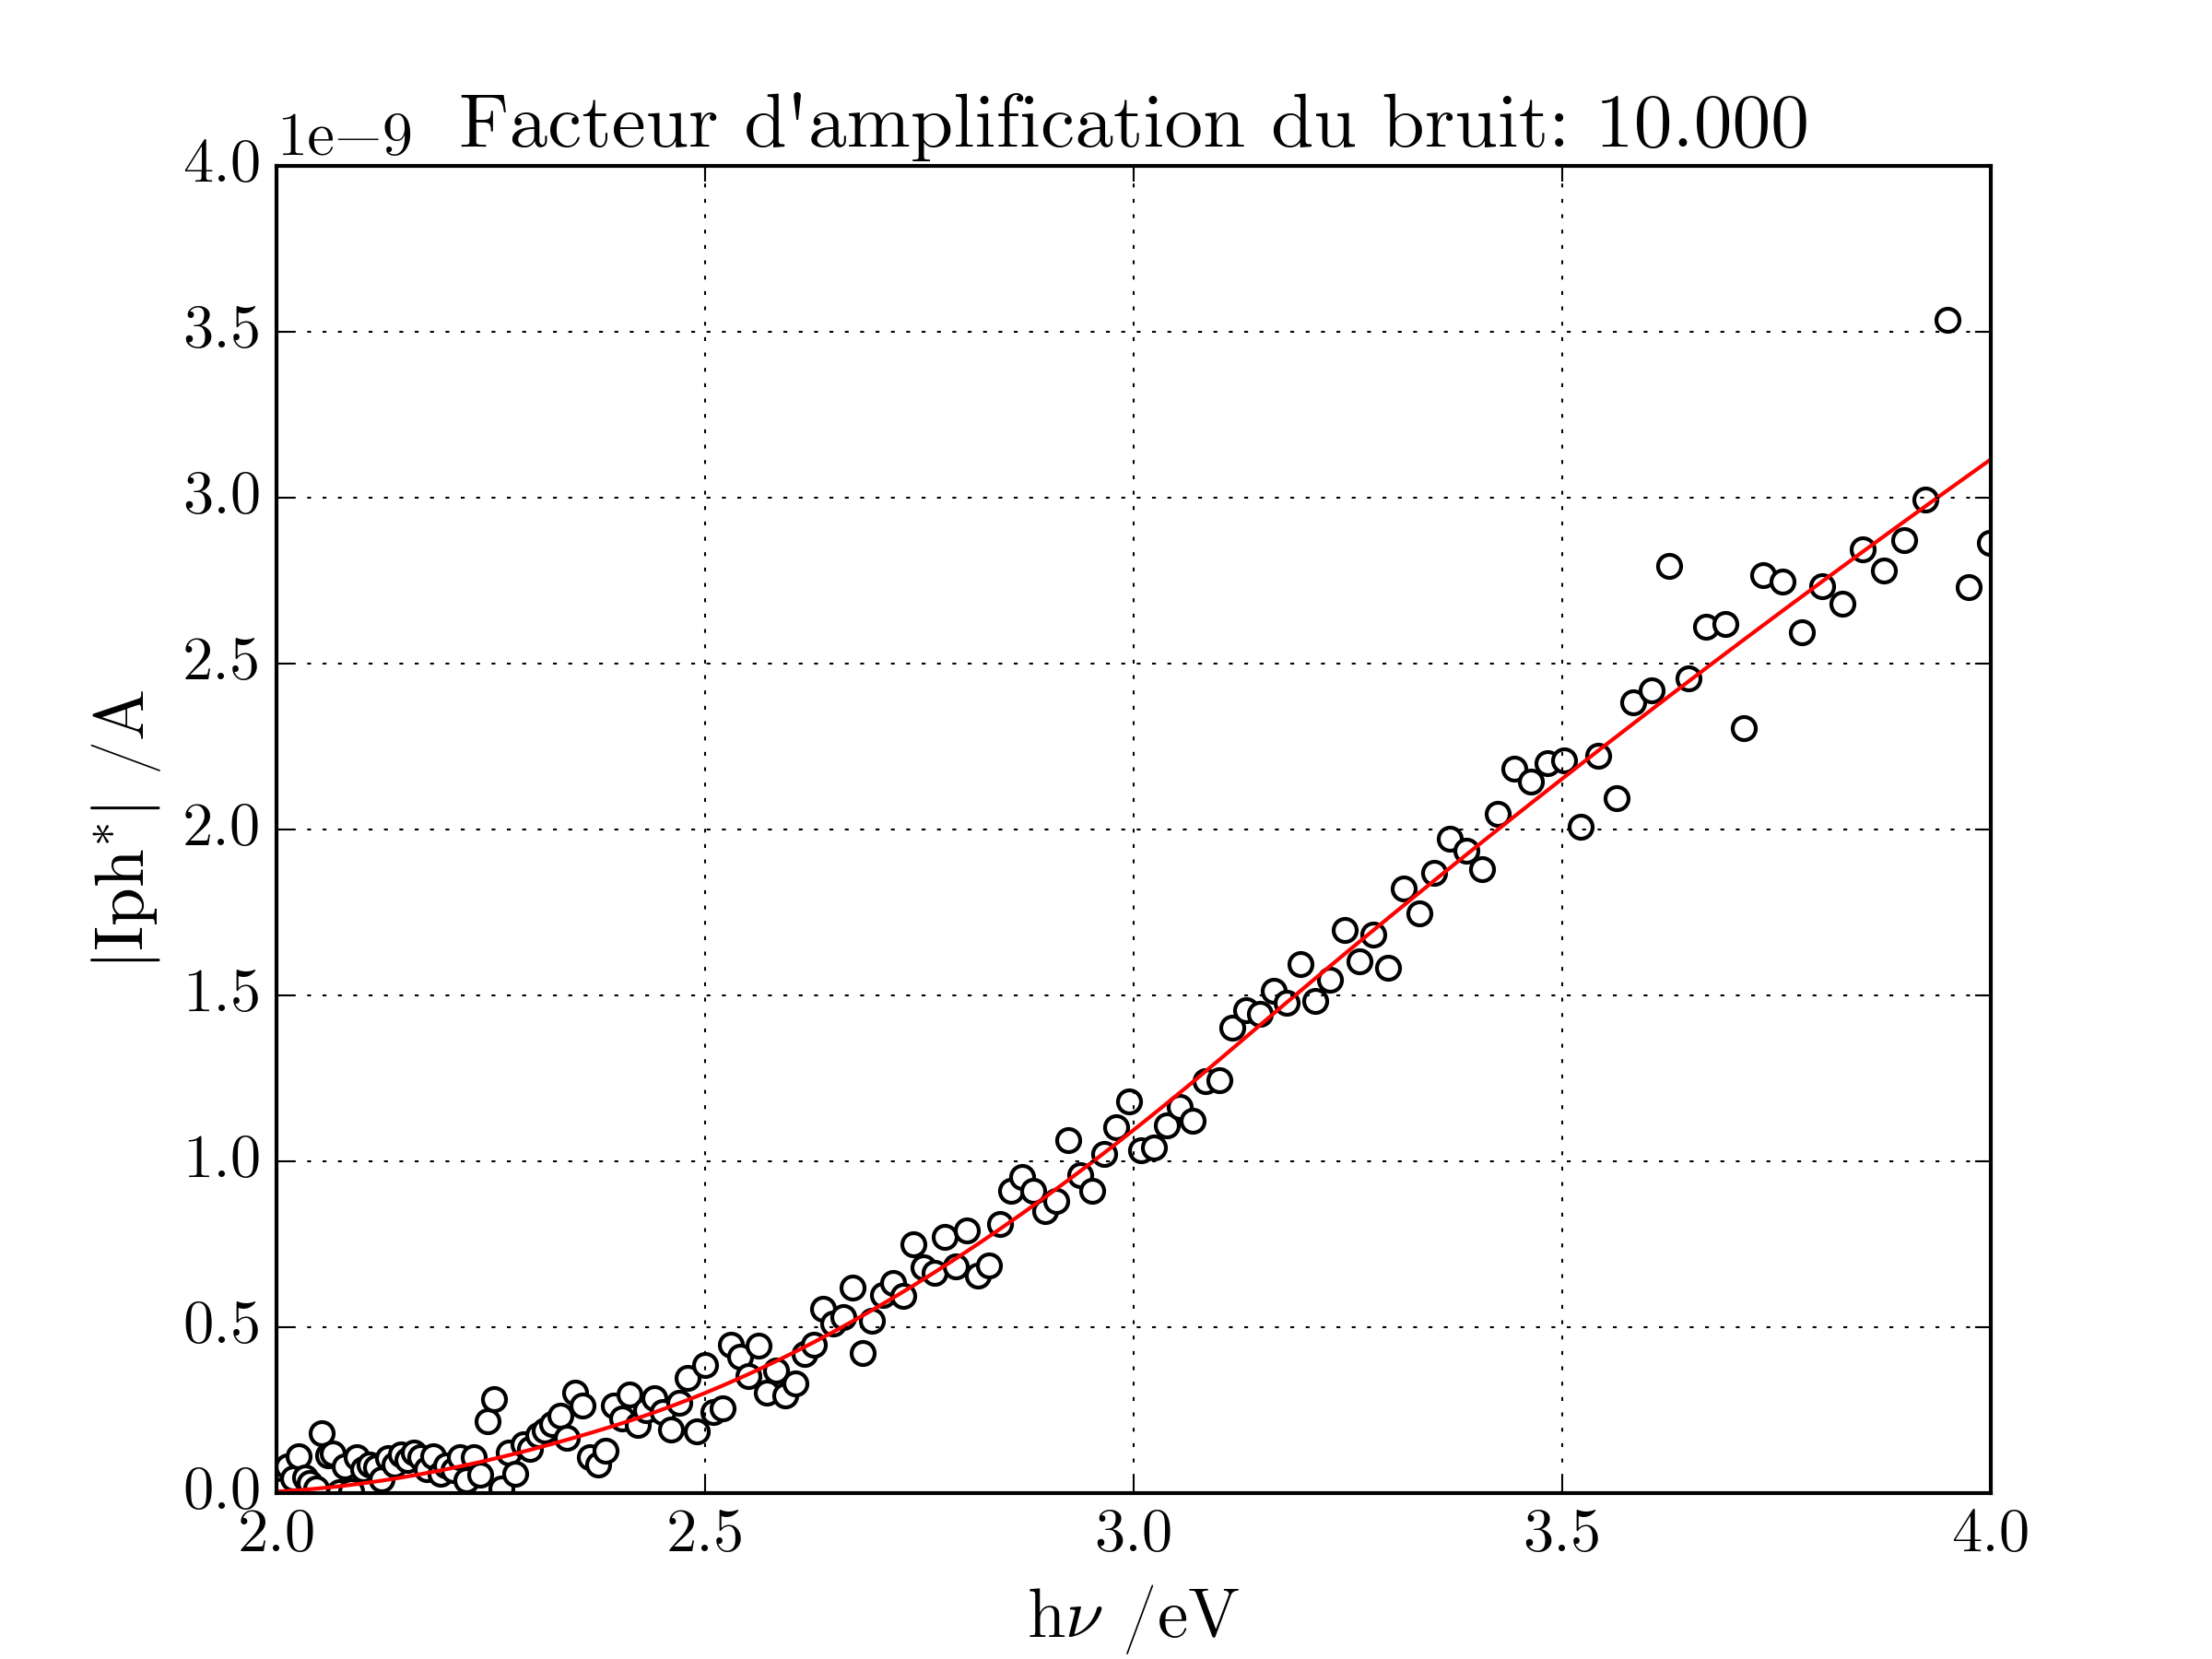
\includegraphics[width=\textwidth]{DSS_0mV_data-Iph-10x.png}
            \caption{}
            \label{}
        \end{subfigure}
        \caption{Photocaractéristiques en énergie générées avec différents facteurs d'amplification du bruit ($f_a$): 
        a) 0.001,
        b) 1,
        c) 2,
        d) 5,
        e) 10.}
        \label{fig:ch3_noise_test}
    \end{figure}

   
    Dans un second temps, les photocaractéristiques en énergie de la figure \ref{fig:ch3_CI_A600_Iph_Ipht} ont été
    utilisées pour tester
    le choix des termes de pondération sur un cas réel où le ratio signal/bruit évolue. Afin de calculer les termes de
    pondération (équation \ref{eq:ch3_weights}) et notamment le bruit moyen $\overline{\epsilon_d}$,
    nous avons choisi de moyenner cinq valeurs du photocourant $\iph$ pour
    les énergies les plus élevées (6.19, 6.17, 6.14, 6.08~eV) où le spectre d'émission de la lampe Xe peut être
    raisonnablement considéré proche de 0. 

    Sur les spectres de la figure \ref{fig:ch3_CI_A600_Iph_Ipht}, 
    le module du photocourant présente une forte 
    diminution pour des énergies inférieures à \SI{3}{\electronvolt} lorsque le potentiel devient de plus en plus
    cathodique, dans ce domaine des basses énergies, le ratio signal/bruit diminue. 
    Le tableau \ref{tab:ch3_fitted_parameters_A600_CI} reprend les valeurs de paramètres présentées dans le tableau
    \ref{tab:ch3_fitted_parameters_A600} en y ajoutant les valeurs obtenues avec notre méthode pour les intervalles de confiance.
    Encore une fois, l'augmentation des intervalles de confiances des trois composantes ayant un gap inférieur à 
    \SI{3}{\electronvolt} reflète la diminution du ratio signal/bruit.
    
    \begin{table}[H] 
        \centering
        \begin{footnotesize}
        \begin{tabular}{l|lll|lll|lll|lll}
            \toprule
            U & $\E_{g,1}$ & $\theta_1$ & $10^{5}K_1$ & $\E_{g,2}$ & $\theta_2$ & $10^{5}K_2$ & $\E_{g,3}$ & $\theta_3$ &
            $10^{5}K_3$ & $\E_{g,4}$ & $\theta_4$ & $10^{5}K_4$\\
            $mV$ & eV & $^{\circ}$ &  & eV & $^{\circ}$ &  & eV & $^{\circ}$ &  & eV & $^{\circ}$ & \\
            \midrule
            \rowcolor{lightgray} & 1.74 & -42.6 & 5.2 & 2.42 & 122 & 6.4 & 2.88 & 134 & 6.54 & 3.47 & -64 & 8.9\\
            \rowcolor{lightgray}\multirow{-2}{*}{100} & ±0.02 & ±0.5 & ±0.1 & ±0.04 & ±2 & ±0.4 & ±0.05 & ±4 & ±0.4 & ±0.06 & ±6 & ±0.8\\ \hline

             & 1.755 & -49.2 & 5.1 & 2.41 & 120 & 6.1 & 2.82 & 131 & 6.8 & 3.48 & -57 & 9.1\\ 
             \multirow{-2}{*}{0} & ±0.008 & ±0.5 & ±0.1 & ±0.04 & ±2 & ±0.4 & ±0.05 & ±4 & ±0.4 & ±0.06 & ±6 & ±0.8\\ \hline

             \rowcolor{lightgray} & 1.76 &  -52.4 & 4.7 & 2.44 & 119 & 6.1 & 2.90 & 131 & 6.9 & 3.43 &  -56 & 9.2 \\
             \rowcolor{lightgray}\multirow{-2}{*}{-100} & ±0.02 &  ±0.5 & ±0.6 & ±0.03 & ±2 & ±0.3 & ±0.04 & ±4 & ±0.4 & ±0.07 &  ±6 & ±0.9 \\ \hline

             & 1.76 &  -53.5 & 4.01 & 2.43 & 121 & 5.07 & 2.85 & 124 & 6.1 & 3.46 &  -63 & 8.3 \\
             \multirow{-2}{*}{-200} & ±0.02 &  ±0.6 & ±0.06 & ±0.04 & ±3 & ±0.4 & ±0.04 & ±4 & ±0.4 & ±0.06 &  ±6 & ±0.6 \\ \hline
                
             \rowcolor{lightgray} & 1.76 &  -52 & 2.9 & 2.42 & 122 & 4.2 & 2.82 & 122 & 5.7 & 3.43 &  -64 & 7.6 \\
             \rowcolor{lightgray}\multirow{-2}{*}{-300} & ±0.05 &  ±2 & ±0.3 & ±0.09 & ±5 & ±0.6 & ±0.07 & ±4 & ±0.5 & ±0.06 &  ±3 & ±0.3 \\ \hline

             & 1.7 & 48 & 1 & 2.4 & 118 & 4 & 2.8 & 126 & 5 & 3.35 &  -61 & 6.7 \\
             \multirow{-2}{*}{-400} & ±0.6 & ±30 & ±2 & ±0.5 & ±20 & ±3 & ±0.3 & ±20 & ±2 & ±0.07 & ±6 & ±0.7 \\
             \bottomrule
        \end{tabular}
        \end{footnotesize}
        \caption[Valeurs des paramètres ajustés pour les photocaractéristiques en énergie de
        la figure \ref{fig:ch3_CI_A600_Iph_Ipht}, et des intervalles de confiance correspondantes.]
        {Valeurs des paramètres ajustés pour les photocaractéristiques en énergie de
        la figure \ref{fig:ch3_CI_A600_Iph_Ipht}, et des intervalles de confiance correspondantes (K en $A^{1/2} eV^{1/2}$).}
        \label{tab:ch3_fitted_parameters_A600_CI}
    \end{table}


    La procédure d'estimation des intervalles de confiance peut également
    apporter un critère supplémentaire dans la détermination du nombre de composantes pour une photocaractéristique en
    énergie. En effet, la détermination du nombre de composantes se fait de manière itérative en ajoutant des composantes
    jusqu'à ce que le spectre du photocourant soit parfaitement ajusté. 
    La connaissance des intervalles de confiance
    permettront d'arrêter le processus itératif lorsque les intervalles de confiances de deux
    composantes se superposent c'est-à-dire qu'elles ne sont plus statiquement discernables, et plus seulement lorsque
    les composantes sont dupliquées.
    
    A titre d'illustration, la photocaractéristique en énergie de la figure \ref{fig:ch3_linear_transform_PEC}a)
    a été ajustée en considérant 3, 4 et 5 composantes semiconductrices entre 
    \SI{1.8}{\electronvolt} et \SI{4.0}{\electronvolt}. 
    Le tableau \ref{tab:ch3_fitted_parameters_2205} présente les
    valeurs des gaps obtenus avec les intervalles de confiance associés. En considérant 3 composantes, les
    trois valeurs de gap obtenues sont toutes discernables. En ajoutant une quatrième contribution, la composante dont le
    gap est \SI{1.91}{\electronvolt} se dédouble en deux composantes (\SI{1.9}{\electronvolt} et \SI{2}{\electronvolt})
    dont la seconde possède une intervalle de confiance du même ordre de grandeur que la valeur elle-même. Cela signifie que
    cette composante supplémentaire n'améliore pas l'ajustement. En ajoutant une cinquième contribution, le même
    dédoublement de la composante, dont le gap est \SI{1.91}{\electronvolt}, est obtenu. De plus, la composante dont le
    gap est \SI{2.4}{\electronvolt} se dédouble également en deux composantes (\SI{2.6}{\electronvolt} et
    \SI{2.7}{\electronvolt}) dont les intervalles de confiances se recouvrent les rendant ainsi statistiquement
    indiscernables. 
    

    \begin{table}[H] 
        \centering
        \rowcolors{2}{}{lightgray}
        \begin{tabular}{p{0.32\textwidth}|%
                        p{0.17\textwidth}%
                        p{0.17\textwidth}%
                        p{0.17\textwidth}}
        \toprule
        Nombre de composantes (m) & 3 & 4 & 5 \\  \midrule
        $E_{g,1}$ /eV & $1.91 \pm 0.07$ & $ 1.9 \pm 0.4 $ & $1.9\pm0.1$ \\
        $E_{g,2}$ /eV & $2.4 \pm 0.2$ & $ 2 \pm 5 $ & $2\pm4$ \\
        $E_{g,3}$ /eV & $3.16 \pm 0.06$ & $ 2.5 \pm 0.4 $ & $2.6\pm0.2$ \\
        $E_{g,4}$ /eV &  & $ 3.14\pm 0.06 $ & $2.7\pm0.2$ \\
        $E_{g,5}$ /eV &  &  & $3.2\pm0.1$ \\
        \bottomrule
        \end{tabular}
        \caption{Valeurs des gaps issues de l'ajustement au modèle du spectre présenté en figure
        \ref{fig:ch3_linear_transform_PEC}a), entre \SI{1.8}{\electronvolt} et \SI{4.0}{\electronvolt}, et les
    intervalles de confiance associés.}
        \label{tab:ch3_fitted_parameters_2205}
    \end{table}

    En conclusion, nous pouvons considérer que le choix des termes de pondération peut être considéré comme pertinent.
    L'estimation des intervalles de confiance que nous proposons permet d'avoir un critère pour
    décider si deux composantes de gaps voisins sont discernables ou non, ce qui est précieux lorsque les photocourants
    sont mesurés sur des couches d'oxydation très complexes, comme par exemple, celles obtenues par \citet{Srisrual2013}
    dans l'équipe SIR de SIMaP pour un alliage base nickel oxydé à \SI{900}{\degreeCelsius} sous oxygène pendant 2~h.

    La figure \ref{fig:ch3_anusara_PEC} montre les spectres en énergie obtenus pour cet échantillon à trois potentiels
    différents. Bien que l'allure des spectres soit très différente d'un potentiel à l'autre, il a été montré que
    chacun des spectres pouvait être représenté par \emph{m} composantes avec un seul jeu de \emph{m} gaps. Mais, pour
    rendre compte correctement des spectres, douze composantes ont été nécessaires. La réalité de la présence d'un si grand
    nombre de composantes a été prouvée par de l'imagerie Raman: l'examen des spectres Raman mesurés en plus de 50000
    spots (diamètre \SI{1}{\micro\meter}) de l'échantillon, traités par analyse en composante principale, puis
    ajustement multi-varié a montré que l'ensemble des spectres résultait de la présence de douze composantes, dont dix
    suffisaient à rendre compte de 99.5~\% des spectres.

    Nous avons eu accès aux données originales correspondantes à ces spectres, et nous les avons ajustés à notre tour au
    modèle. Clairement, nous avons trouvé à notre tour la nécessité d'utiliser douze composantes. Le tableau
    \ref{tab:ch3_anusara_PEC} montre
    les valeurs de gaps obtenus à chaque potentiel. L'analyse combinée des intervalles de confiance déterminés à chacun
    des potentiels permet de conclure que, même si certains gaps sont voisins, toutes les composantes sont discernables.

    \newpage
    \begin{figure}[H]
        \centering
        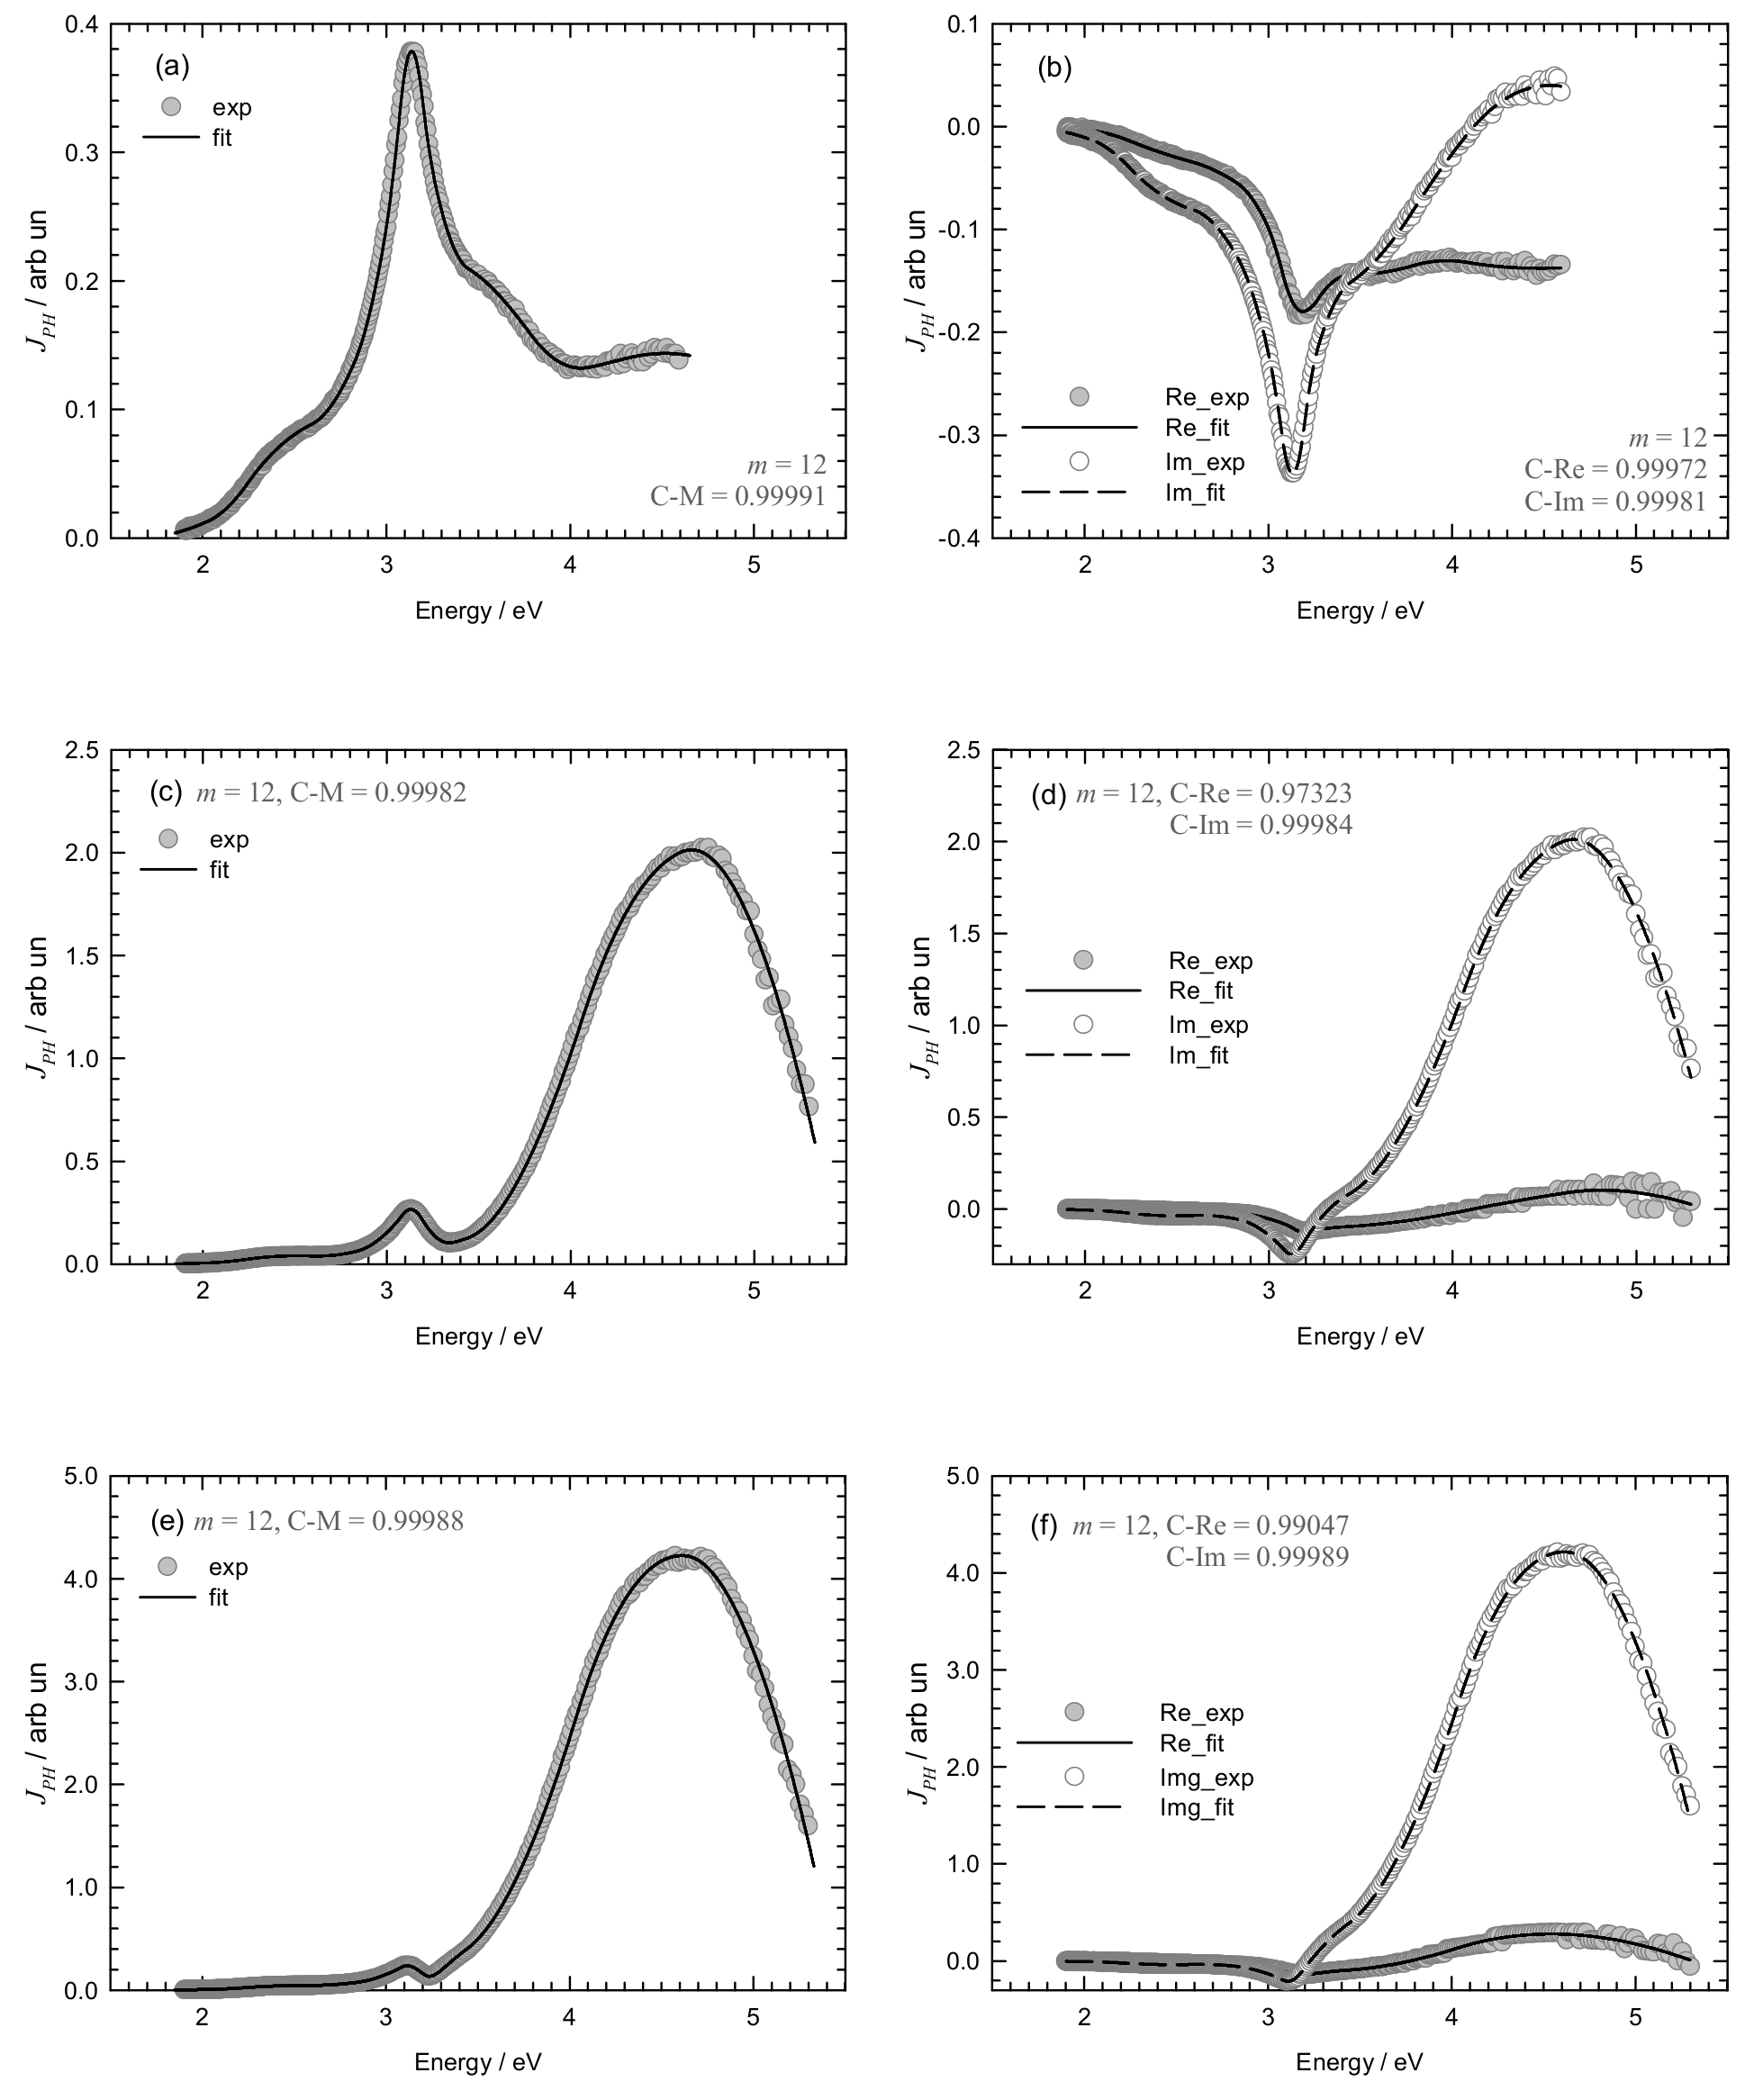
\includegraphics[width=\textwidth]{Srisrual_2013-Fig4_37.png}
        \caption[Spectres en énergie de photocourants mesurés sur un alliage de nickel A690 oxydé à \SI{900}{\degreeCelsius}
        sous oxygène pendant 2~h pour différents potentiels appliqués:
        a) $\SI{0}{\milli\volt}_{MSE}$,
        b) $\SI{-300}{\milli\volt}_{MSE}$,
        c) $\SI{-600}{\milli\volt}_{MSE}$. "Re" et "Im" symbolisent les parties réelle et imaginaire du photocourant
        $J_{ph}$.]
        {Spectres en énergie de photocourants mesurés sur un alliage de nickel A690 oxydé à \SI{900}{\degreeCelsius}
        sous oxygène pendant 2~h pour différents potentiels appliqués (d'après \citet{Srisrual2013}):
        a) $\SI{0}{\milli\volt}_{MSE}$,
        b) $\SI{-300}{\milli\volt}_{MSE}$,
        c) $\SI{-600}{\milli\volt}_{MSE}$. "Re" et "Im" symbolisent les parties réelle et imaginaire du photocourant
        $J_{ph}$.}
        \label{fig:ch3_anusara_PEC}
    \end{figure}
    \newpage


    \begin{table}[H]
        \centering
        \rowcolors{2}{}{lightgray}
        \begin{tabular}{p{0.15\textwidth}|p{0.2\textwidth}%
                            p{0.2\textwidth}%
                            p{0.2\textwidth}}
            \toprule
            & 0~$mV_{MSE}$ & -300~$mV_{MSE}$ & -600~$mV_{MSE}$\\\midrule
            $E_{g,1}$ /eV & 1.7±0.2 & 2±3 & 2±20\\
            $E_{g,2}$ /eV& 2.0±0.2 & 2±3 & 2±8\\
            $E_{g,3}$ /eV& 2.25±0.07 & 2±1 & 2±4\\
            $E_{g,4}$ /eV& 2.58±0.03 & 2.6±0.3 & 2±2\\
            $E_{g,5}$ /eV& 2.80±0.04 & 2.9±0.2 & 2.8±0.9\\
            $E_{g,6}$ /eV& 2.96±0.02 & 3.08±0.01 & 3.09±0.05\\
            $E_{g,7}$ /eV& 3.080±0.002 & 3.16±0.03 & 3.2±0.2\\
            $E_{g,8}$ /eV& 3.200±0.003 & 3.19±0.02 & 3.20±0.05\\
            $E_{g,9}$ /eV& 3.27±0.02 & 3.42±0.03 & 3.42±0.04\\
            $E_{g,10}$ /eV& 3.44±0.03 & 4.070±0.009 & 4.050±0.008\\
            $E_{g,11}$ /eV& 3.8±0.3 & 4.7±0.1 & 4.8±0.2\\
            $E_{g,12}$ /eV& 4.1±0.5 & --- & --- \\
        \bottomrule
    \end{tabular}
    \caption{Valeurs de gaps obtenues par ajustement des spectres en énergie de la figure \ref{fig:ch3_anusara_PEC}, et
            les intervalles de confiance associés}.
    \label{tab:ch3_anusara_PEC}
    \end{table}    
    
    
\section{Cellule électrochimique}\label{sec:ch3_cell}

    \subsection{Description générale}\label{subsec:cell_global_overview}

        La cellule électrochimique haute température équipée d’un hublot optiquement transparent a été développée au Centre Technique du Creusot afin de répondre
        aux exigences en termes de sécurité liées au travail à haute température et haute pression c’est-à-dire
        \SI{280}{\degreeCelsius} et \SI{80}{\bar}.
        Dans la suite, cette cellule électrochimique sera dénommée \emph{cellule HTP}.
        
        La figure \ref{fig:3D_HT_cell} présente une vue en perspective de la cellule HTP.
        Elle est constituée de trois pièces maîtresses : \emph{le corps de cellule}, \emph{le hublot en saphir}, et 
        \emph{le porte-échantillon}. L'étude préalable pour le choix du matériau du hublot ainsi que la description détaillée du
        porte-échantillon sont abordées dans les paragraphes \ref{subsec:window_material} et
        \ref{subsec:sample_holder_electrodes}, respectivement.
        L'ensemble des pièces métalliques a été réalisé en acier inoxydable 304L. 

        \begin{figure}[H]
            \centering
            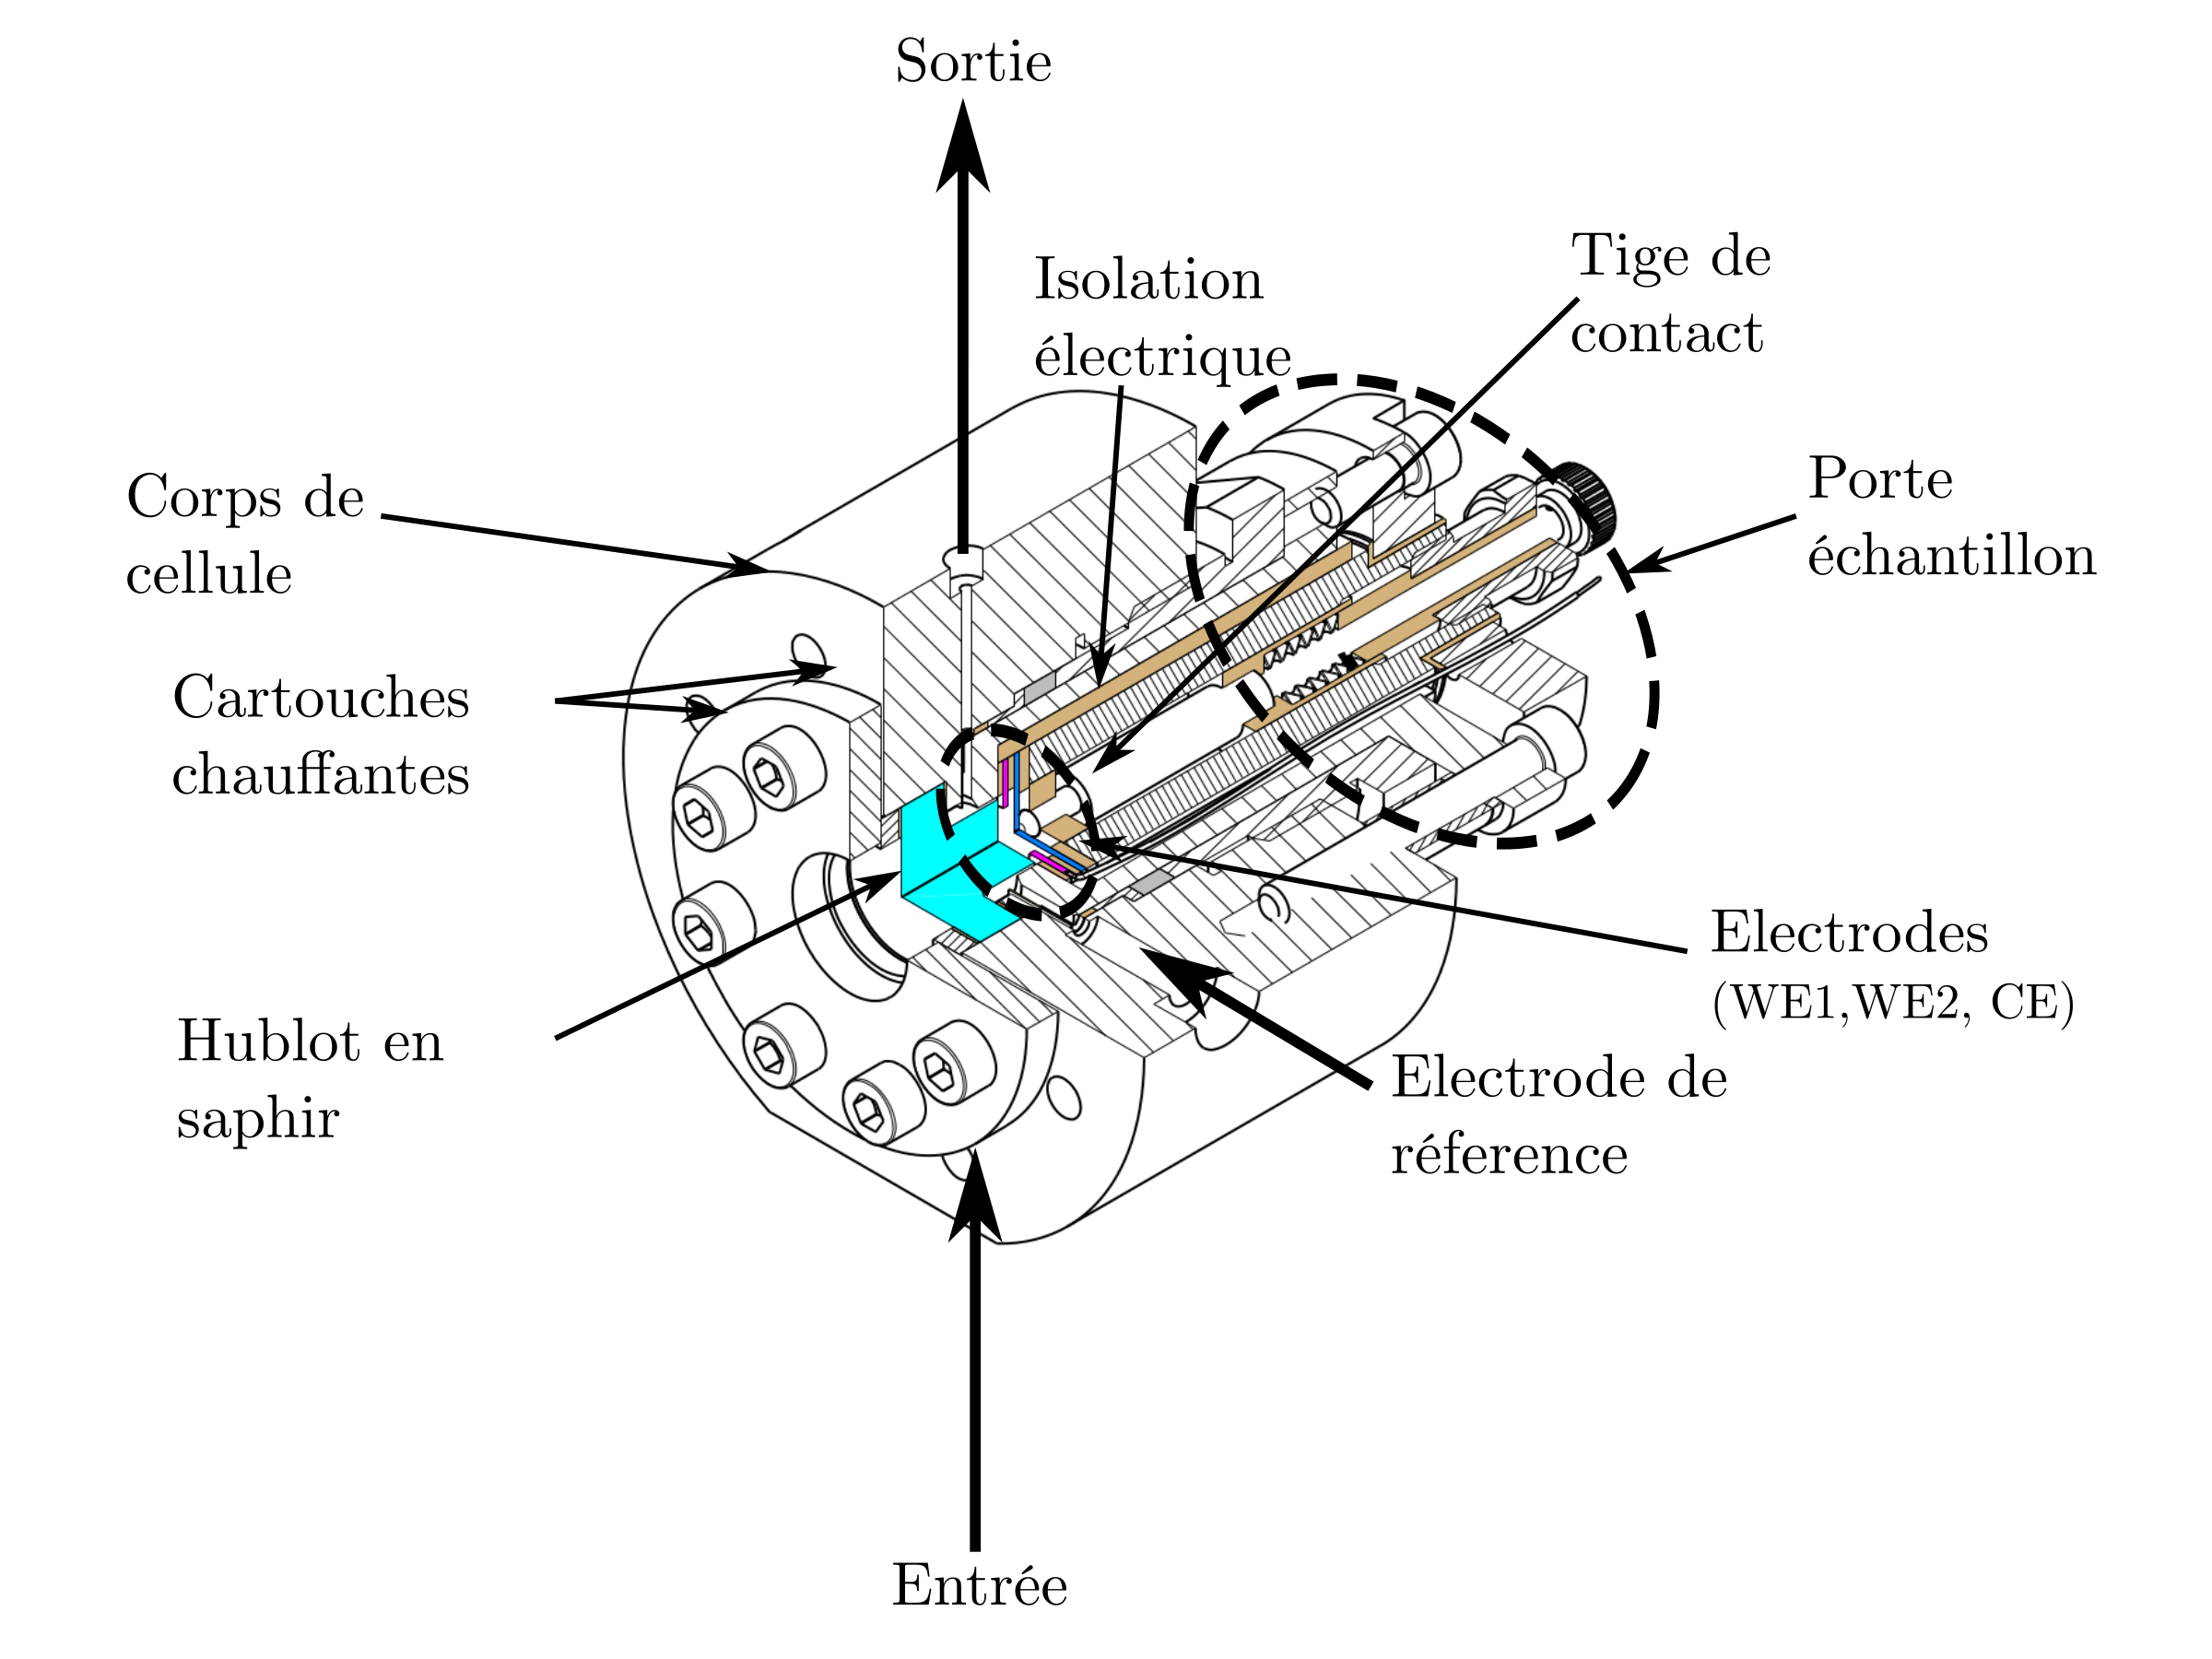
\includegraphics[width=0.85\textwidth]{Shadow_Cell-T_Sapphire-3D.png}
            \caption{Vue en perspective de la cellule HTP avec un aperçu de l’intérieur de la cellule.}
            \label{fig:3D_HT_cell}
        \end{figure}

        Le corps de la cellule HTP est équipé d’une entrée et d’une sortie permettant de faire circuler l’électrolyte.
        Un passage étanche positionné perpendiculairement au flux d’électrolyte permet d’insérer une électrode de
        référence Ag/AgCl. 
        Des emplacements pour les cartouches chauffantes sont positionnés sur la périphérie du corps de la cellule.
        La profondeur des emplacements permet aux cartouches chauffantes de traverser tout le corps de la cellule. 

        Le hublot assure le passage du flux lumineux provenant de la source jusqu’à la surface de
        l’échantillon. La forme en "T" du hublot permet de minimiser la distance d'eau à traverser et ainsi de minimiser
        l'absorption du flux de photons par l'électrolyte.
        Le faisceau traverse ainsi une distance de \SI{16}{\milli\meter} de saphir puis une distance de
        \SI{3}{\milli\meter} d'eau seulement avant d'atteindre la surface de l'échantillon. 

        Le porte-échantillon permet de positionner les électrodes en face du hublot tout en assurant 
        l’étanchéité des contacts ainsi que l’isolation électrique de ces derniers par rapport au corps de la cellule
        HTP.
        L’isolation électrique et l’étanchéité sont assurées par des pièces en (PEEK) dont 
        les propriétés physico-chimiques sont adaptées aux conditions d’utilisation de la cellule HTP.


     \subsection{Choix du matériau du hublot}\label{subsec:window_material}

        Afin de pouvoir illuminer les échantillons dans la cellule HTP, il est nécessaire d'utiliser un 
        matériau résistant aux contraintes mécaniques imposées par le milieu pressurisé à \SI{80}{\bar}, résistant à
        la chimie du milieu et ainsi transparent dans le domaine des ultraviolets.
        Le saphir est composé d'alumine stable $\alpha$ appelée \emph{corundum} 
        et est doté d'excellentes propriétés de transparence optique dans le domaine des UV.
        De plus, les propriétés mécaniques du saphir monocristallin en font un matériau de choix. 
        En effet, celui-ci possède une valeur minimale de résistance à la flexion 
        $\rm \sigma _f$ de \SI{480}{\mega\pascal} \citep{Pishchik2009}. 
        Cependant, lorsque ce dernier est immergé en solution aqueuse, des hydroxydes d'aluminium peuvent se
        former en surface : \emph{gibsite}, \emph{bayerite}. Il peut également y avoir formation de hydroxyde 
        d'aluminium tel que la \emph{boehmite} et la \emph{diaspore} entraînant l'opacification de la 
        surface \citep{Pishchik2009,Franks2007}.

        Les propriétés de l'alumine qui vont conditionner la formation ou non d'hydroxydes sont sa pureté,
        ses défauts cristallins et son état de surface. Pour minimiser la probabilité de formation d'hydroxydes,
        des saphirs monocristallins orientés 0001 (plan C, aussi appelé axe optique), sont utilisés. 
        Deux fournisseurs de saphir ont été sélectionnés : Neyco et Roditi, avec une pureté annoncée de l'alumine  
        de 96~\% et 99.995~\%, respectivement et les mêmes dimensions c'est-à-dire un diamètre de 10~mm et une
        épaisseur de 5~mm.
        Les impuretés peuvent créer des défauts dans le monocristal qui vont ensuite migrer 
        jusqu'à la surface avec d'autant plus de facilité que la température augmente. 
        Ces défauts ont une énergie plus importante et sont susceptibles de réagir avec l'eau favorisant
        ainsi la formation de groupes hydroxyles en surface \citep{Franks2007}.

        Des hublots de saphir pré-sélectionnés ont été vieillis dans un environnement REB désaéré c'est-à-dire dans de 
        l'eau ultra pure désaérée (par bullage d'argon) à \SI{280}{\degreeCelsius} et sous une pression de \SI{80}{\bar}.
        Ces vieillissements ont été réalisés de manière séquentielle dans les capsules c'est-à-dire qu'un premier vieillissement
        d'environ \SI{1100}{\hour} est réalisé suivi d'un deuxième vieillissement d'environ \SI{330}{\hour} et enfin 
        d'un dernier vieillissement d'environ \SI{310}{\hour}. La solution de vieillissement a été prélevée pour analyse après chaque 
        vieillissement et de l'eau-ultra pure désaérée a été utilisée pour le vieillissement suivant.
        La figure \ref{fig:comparison_new_aged} montre les spectres de transmission des hublots de saphir testés dans le 
        domaine d'énergie allant de \SI{1.2}{\electronvolt} à \SI{6.5}{\electronvolt}.
        
        \begin{figure}[H]
        \centering
            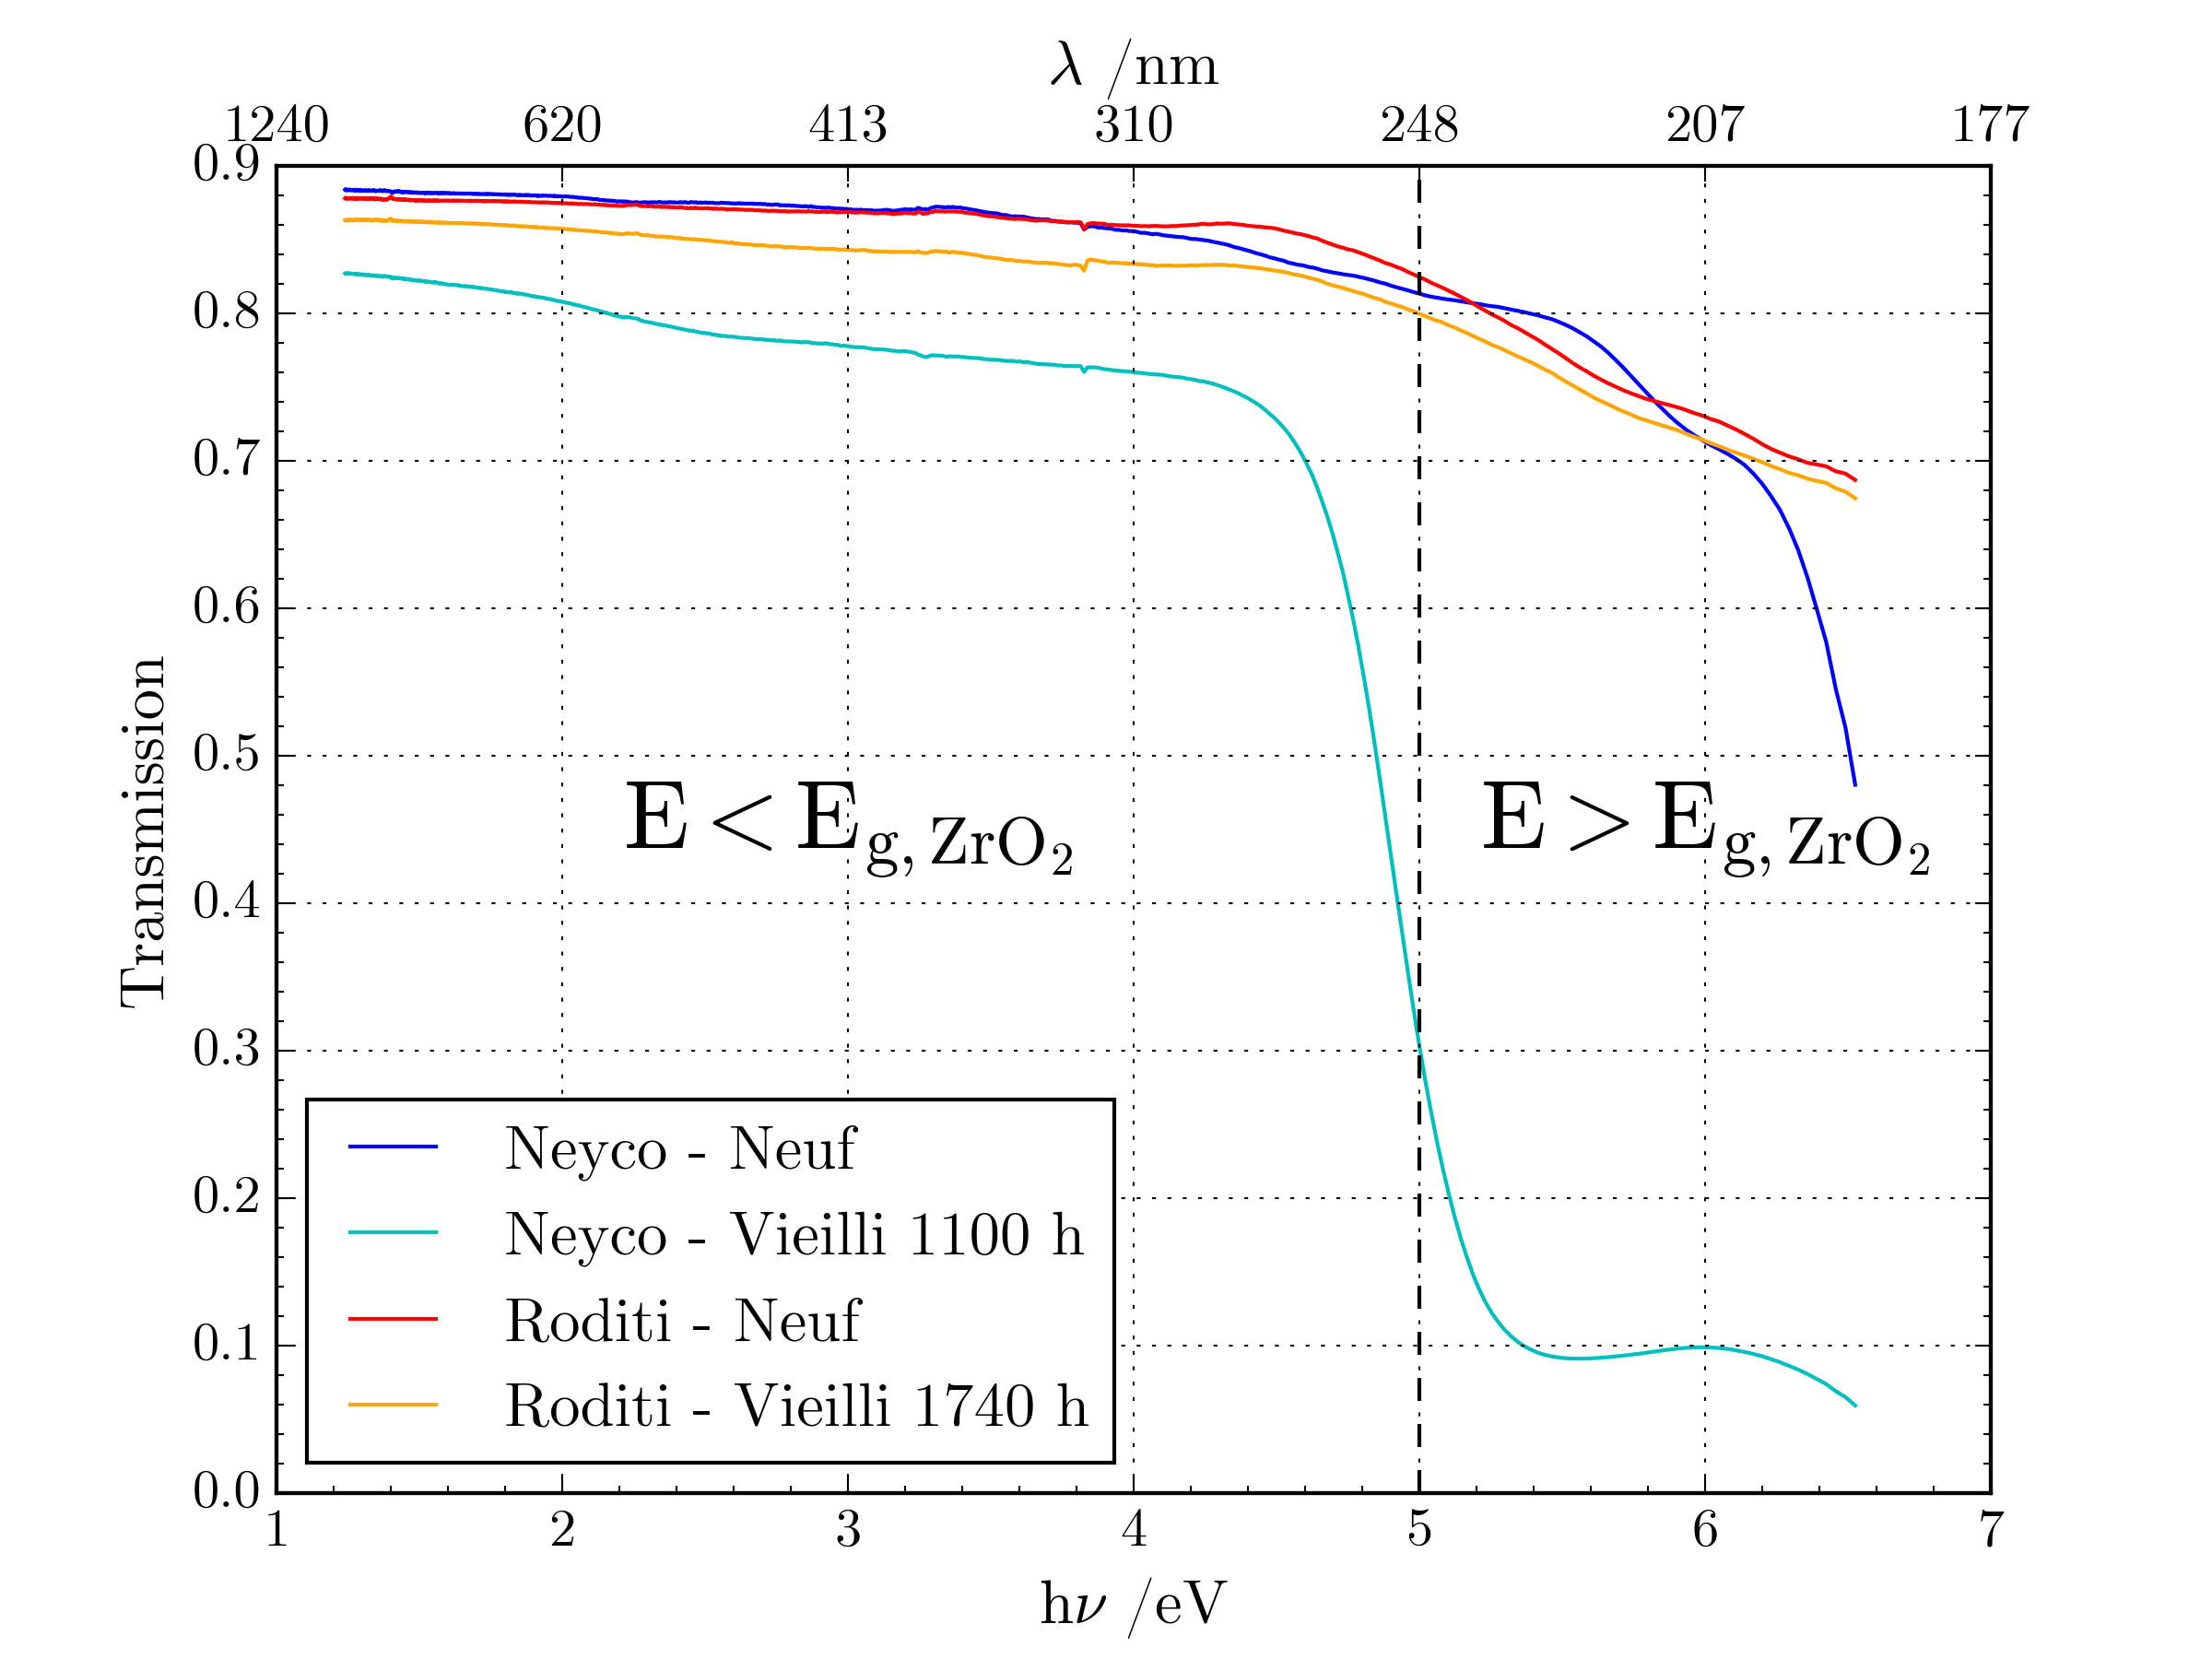
\includegraphics[width=0.85\textwidth]{130008-New_vs_Aged.png}
            \caption{Spectres de transmission entre
            \SI{1.2}{\electronvolt} et \SI{6.5}{\electronvolt} des hublots de saphir des fournisseurs Neyco et Roditi avant
            et après vieillissement.}
            \label{fig:comparison_new_aged}
        \end{figure}
        
        A l'état neuf, les spectres de transmission des deux saphirs testés sont similaires entre 
        \SI{1.2}{\electronvolt} et \SI{5.6}{\electronvolt}. Le saphir Roditi présente une meilleure transmission 
        pour des énergies supérieures à \SI{5.6}{\electronvolt}. Cette différence est probablement liée à la différence
        de
        pureté des deux saphirs. Le saphir Neyco présente une forte dégradation de la transmission après \SI{1100}{\hour}
        de vieillissement pour des énergies supérieures à \SI{4.1}{\electronvolt}. En revanche, la transmission
        du saphir Roditi est quasiment inchangée même après un vieillissement de \SI{1740}{\hour}.
        La cellule HTP a en conséquence été équipée d’un hublot de saphir fourni par Roditi.
        Contrairement à ce qui a été pratiqué par d'autres auteurs \citep{Kim2010}, aucun revêtement protecteur
        supplémentaire n'a été nécessaire ici.
       
        
    \subsection{Porte-échantillon et électrodes}\label{subsec:sample_holder_electrodes}

        La figure \ref{fig:Profile_HT_cell} illustre les éléments évoqués précédemment dans une vue en profil 
        de la cellule HTP afin de mieux visualiser les éléments du porte-échantillon. 
        Le plan de la coupe est le plan perpendiculaire à l’axe de passage de l’électrolyte. 
        Le dispositif complet se présente comme une cellule électrochimique à 4 électrodes dont 2 électrodes de travail,
        une contre-électrode et une électrode de référence.

        \begin{figure}[H]
            \centering
            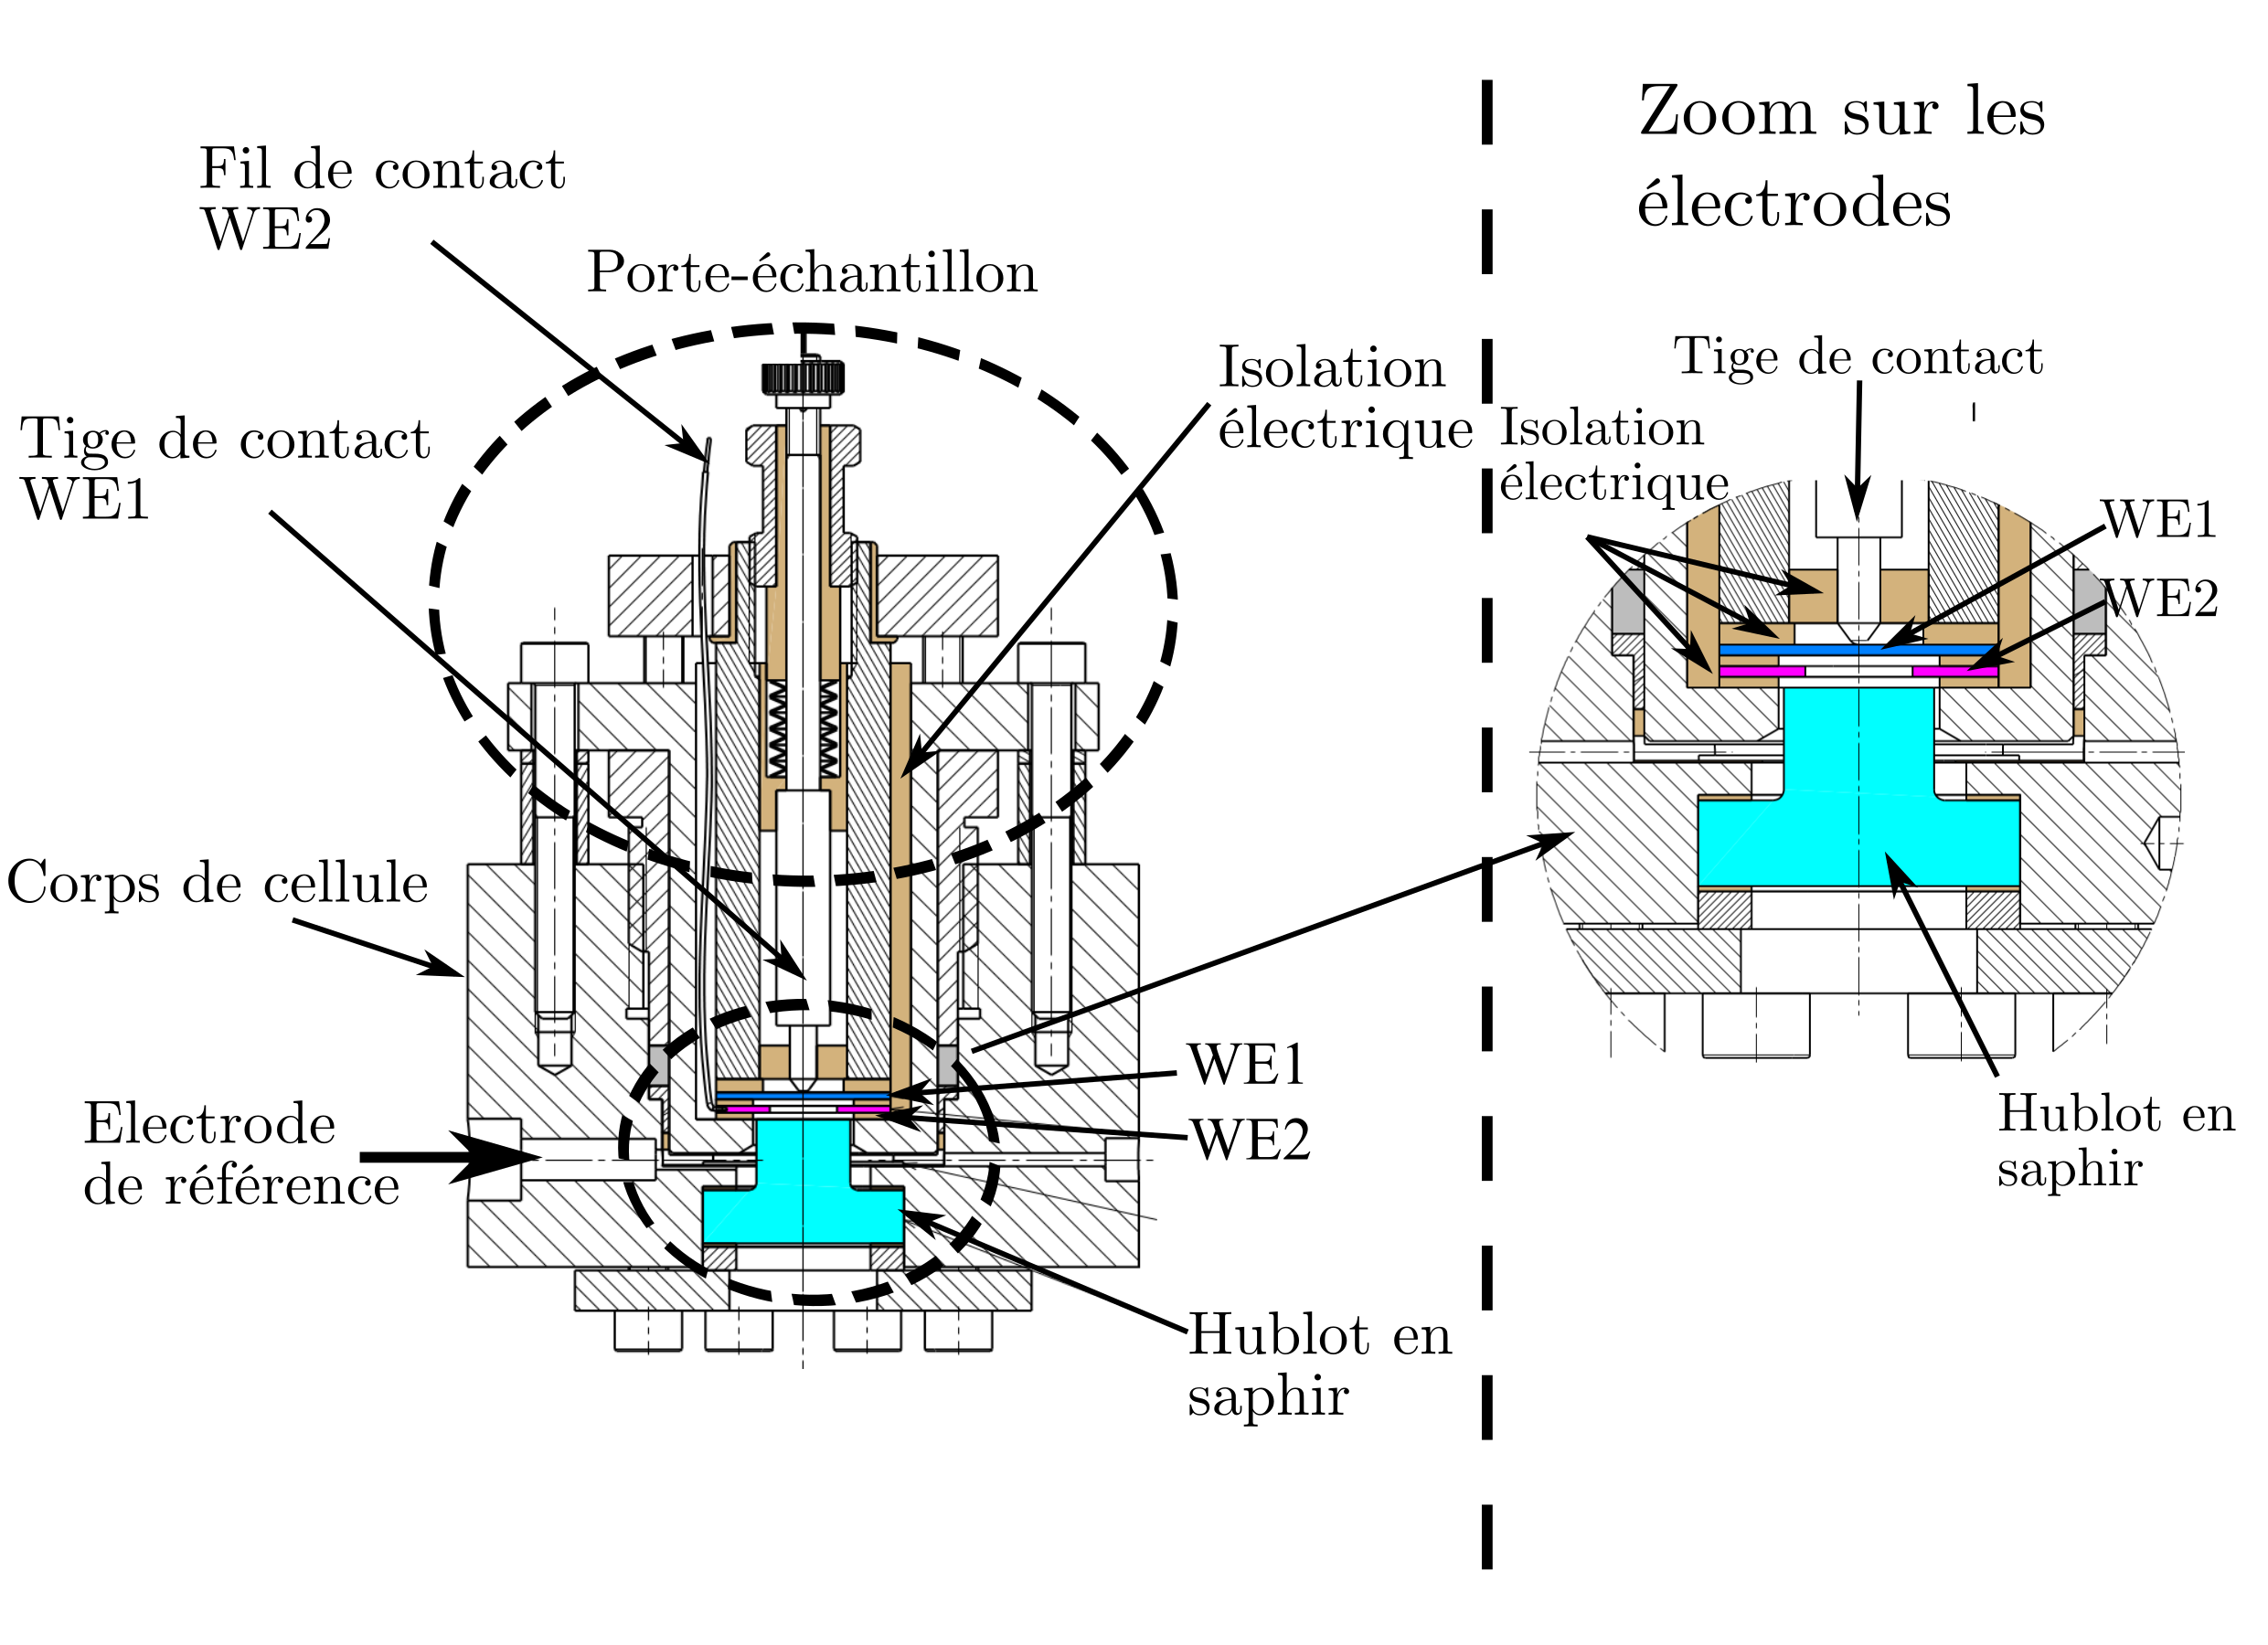
\includegraphics[width=0.85\textwidth]{Shadow_Cell-T_Sapphire-Profile.png}
            \caption{Plan en coupe de la cellule HTP.}
            \label{fig:Profile_HT_cell}
        \end{figure}


        L’électrode de travail n°1 (WE1) est disque plein ayant un diamètre de \SI{26}{\milli\meter} 
        dont le contact électrique avec l'extérieur est assuré par une tige métallique en appui physique sur l’arrière 
        de l’électrode. Cette tige peut être tournée sur elle-même afin de renouveler la surface du contact arrière de
        l'échantillon. 
        En effet, la face arrière de l’électrode est exposée à l’atmosphère ambiante et s’oxyde au cours du 
        temps lorsque la cellule HTP est à température de fonctionnement nominal. 
        Cette électrode de travail assure le contrôle de la surface exposée sans effet de bord et elle reçoit le maximum
        de flux lumineux à travers le hublot en saphir. 
        L'alliage Zy2 a majoritairement été utilisé en tant qu'électrode de travail n°1, mais pas uniquement.

        L’électrode de travail n°2 (WE2) est un anneau avec des diamètres extérieur et intérieur 
        de \SI{26}{\milli\meter} et \SI{10}{\milli\meter}, respectivement. 
        Le contact électrique est assuré par un fil soudé par point sur l’extérieur de l’anneau. 
        Le matériau utilisé pour le contact électrique est de même nature que le matériau de l’électrode, le plus
        souvent un Inc718.
        La distance entre les électrodes de travail 1 et 2 est fixée par la taille de l'anneau en PEEK assurant l'étanchéité
        et l'isolation électrique. L'épaisseur de ce dernier est de \SI{1}{\milli\meter}.
        A la différence de l'électrode de travail n°1, cette électrode reçoit
        beaucoup moins de flux lumineux. De plus, les effets de bords, liés à la géométrie, ne sont pas négligeables.
        %Par conséquent, l'électrode de travail n°2 est principalement utilisée pour la mesure directe du courant de
        %couplage en étant couplée avec l'électrode de travail n°1.

        Le choix initial de doter la cellule de deux électrodes de travail a été fait pour permettre de polariser Zy2 et
        Inc718 à des potentiels choisis par l'utilisateur pour favoriser ou défavoriser le couplage galvanique.
        Malheureusement, il n'a pas été possible de trouver dans le commerce un bipotentiostat capable de fonctionner en
        mode flottant.

        La contre-électrode (CE) est également un anneau avec des diamètres extérieur et intérieur 
        de \SI{30}{\milli\meter} et \SI{13}{\milli\meter}, respectivement. 
        Comme pour l’électrode de travail n°2, le contact électrique est assuré par un fil soudé par point.
        A la différence de l’électrode de travail n°2, le contact se trouve exposé à l’électrolyte et par conséquent,
        la nature du matériau du fil de contact doit absolument être identique à celle de l’électrode. 
        Le platine a été choisi comme matériau de la contre-électrode, de manière à disposer si nécessaire d'une
        (pseudo-)référence supplémentaire en milieu désaéré.
        On notera également que le corps de cellule HTP peut être utilisé comme contre-électrode.
        
        

	
%%%%%%%%%%%%%%%%%%%%%%%%%%%%%%%%%%%%%%%%%%%%%%%%%%%%%%%%%%%%%%%%%%%
\section{Cellule double hublot}\label{sec:2W_cell}

    La mesure de spectres en énergie de photocourants nécessite de réaliser des "spectres de lampes" afin de pouvoir
    "corriger" le
    photocourant brut du flux de photons incident à chaque énergie (voir \S\ref{subsec:ch3_interpretation_PEC}).
    Nous avons donc voulu  reproduire à la même température les milieux traversés (air-saphir-eau)
    par le faisceau lumineux avant d'atteindre la
    surface de l'échantillon tout en ayant la possibilité de positionner la photodiode permettant de mesurer les flux.
    Nous avons donc developpé
    une cellule symétrique permettant de placer deux hublots l'un en face de l'autre avec une circulation d'électrolyte
    entre les deux.

    Tout comme la cellule HTP, la cellule double hublot possède une entrée et une sortie pour la circulation de
    l'électrolyte et le chauffage est également assuré par des cartouches chauffantes.
    La figure \ref{fig:two_window_cell} présente une vue en perspective de la géométrie de cette cellule
    qui sera nommé dans la suite \emph{cellule double hublot}. 
    Chaque hublot a une épaisseur de \SI{8}{\milli\meter} et la distance entre les deux hublots a été fixée à
    \SI{3}{\milli\meter} c'est-à-dire la distance saphir--échantillon dans la cellule HTP.
    
    \begin{figure}[H]
		\centering
		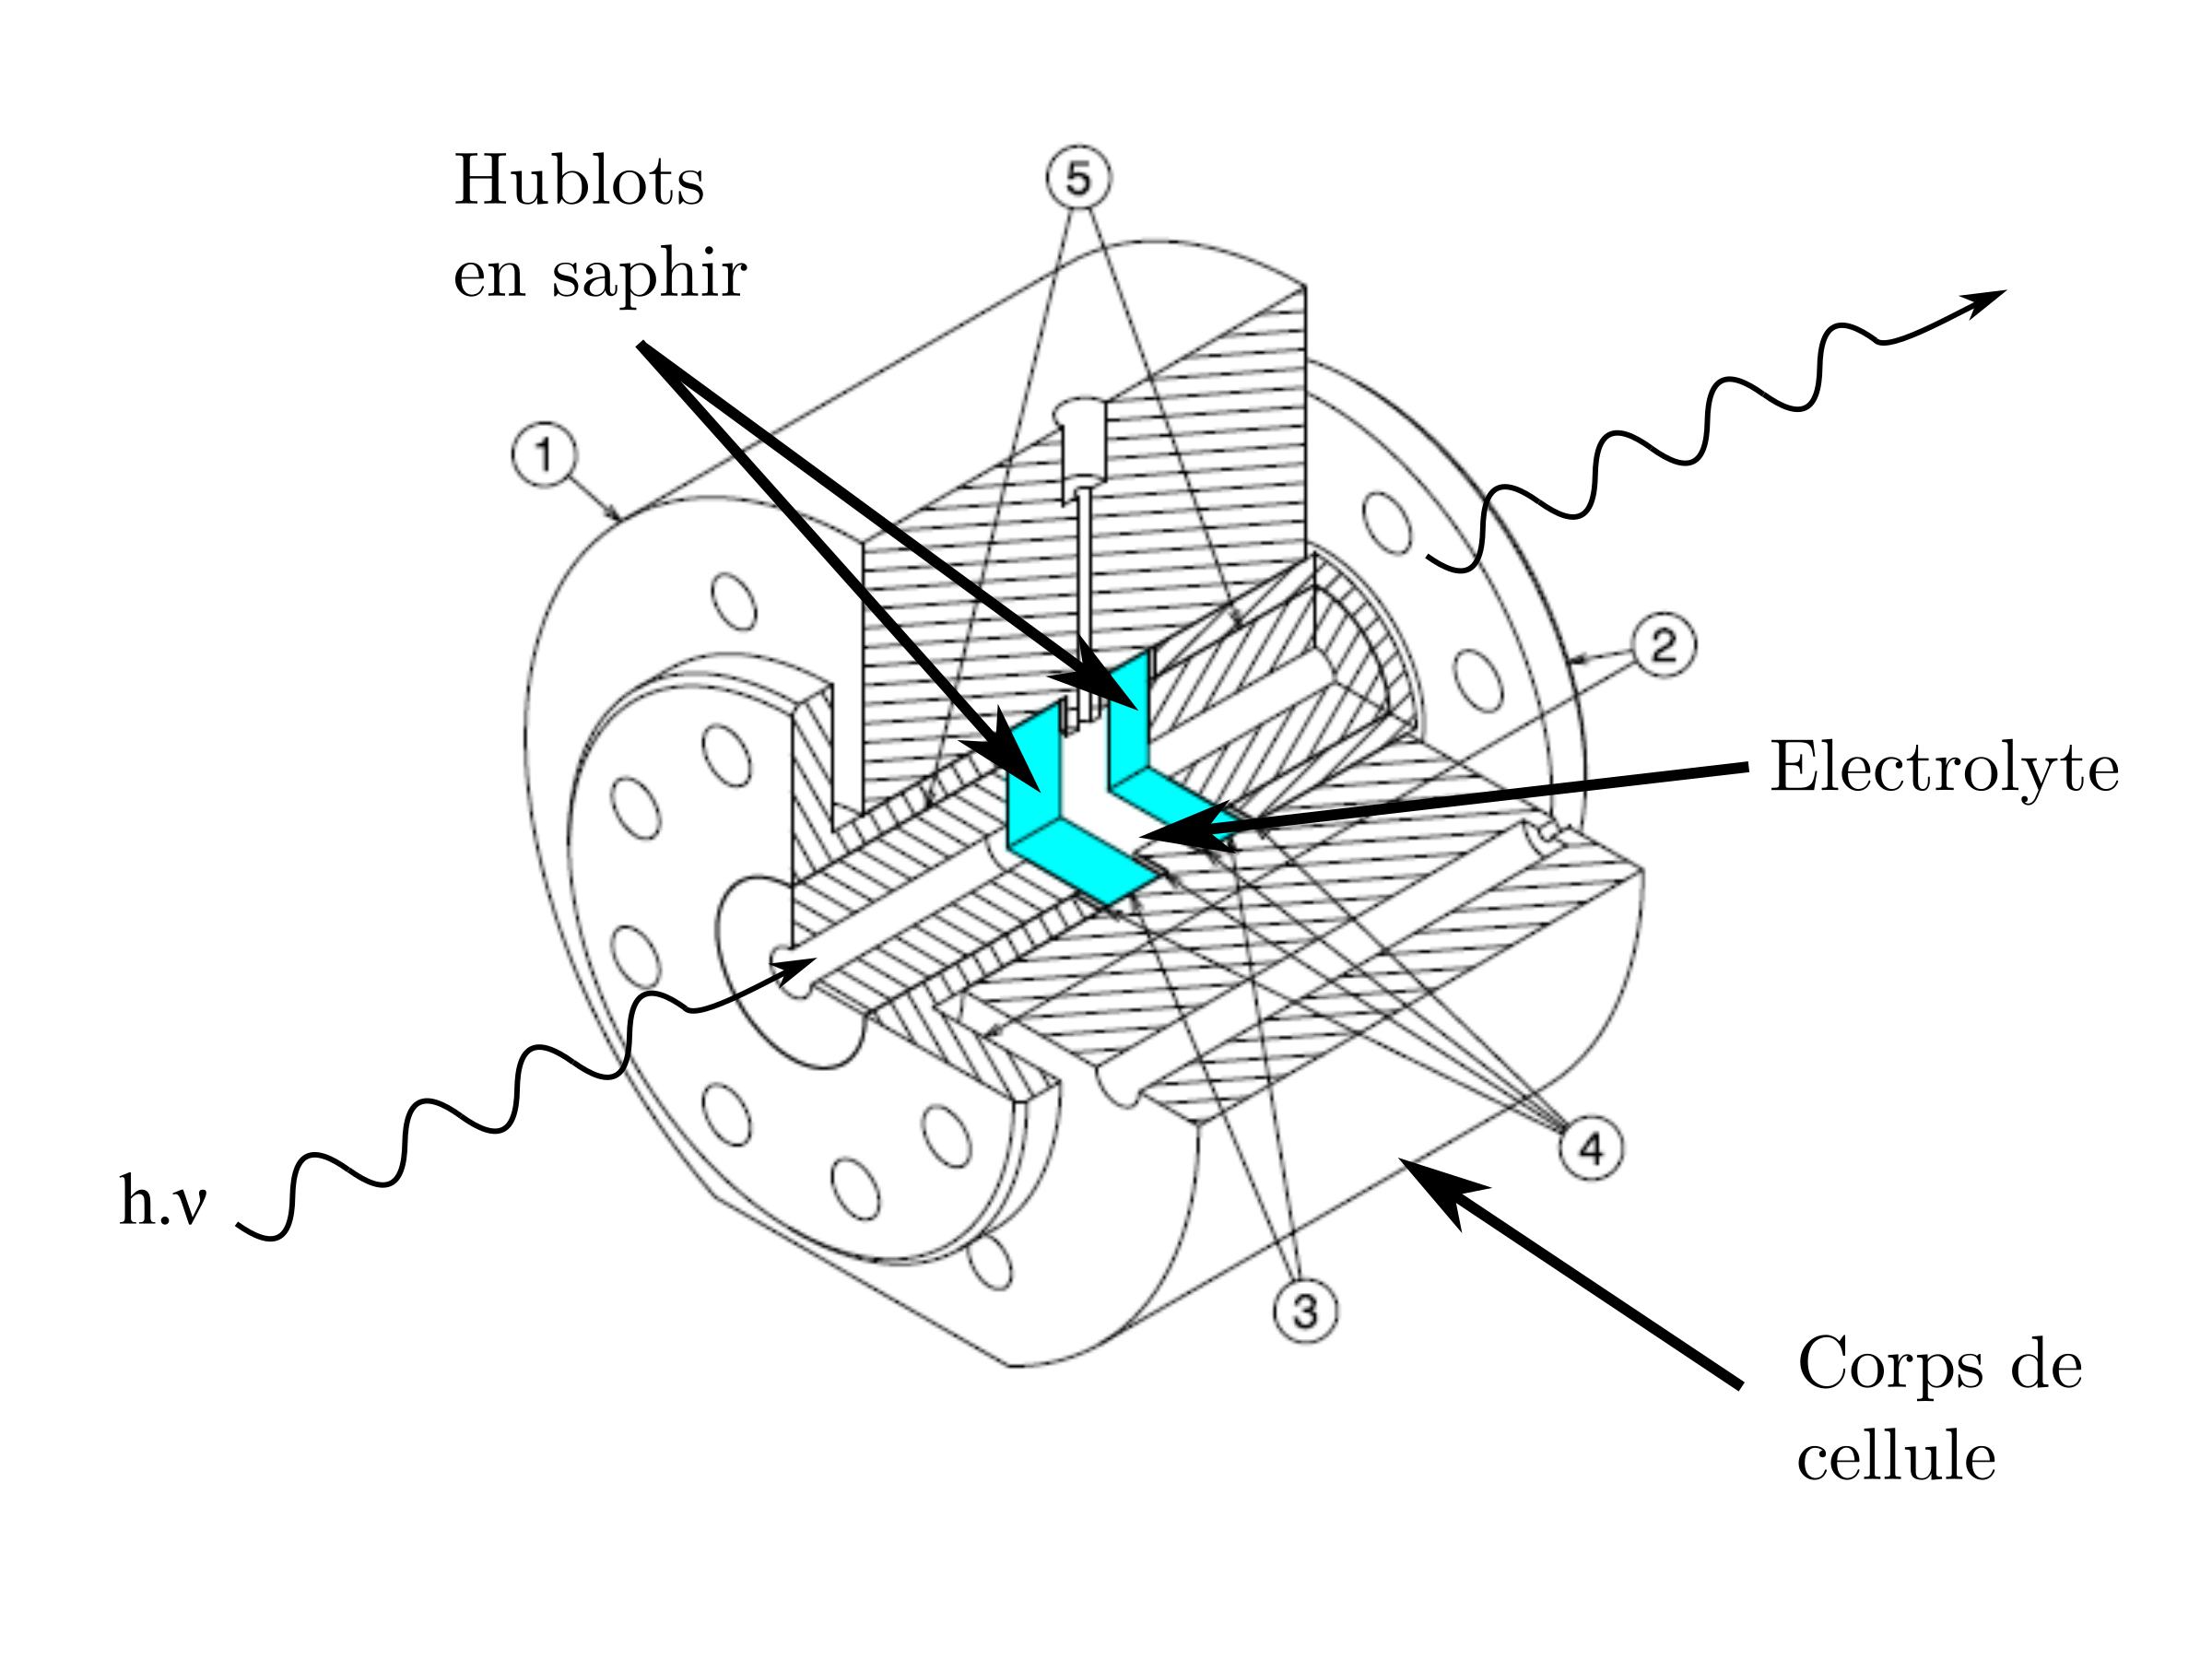
\includegraphics[width=0.65\textwidth]{2Window_Cell.png}
		\caption{Vue en perspective de la cellule double hublot.}
		\label{fig:two_window_cell}
	\end{figure}
    
    Avec ce choix de design, le faisceau lumineux traverse une épaisseur identique de saphir que pour la cellule HTP
    comme illustré en figure \ref{fig:ch3_optical_paths}.

    \begin{figure}[H]
		\centering
		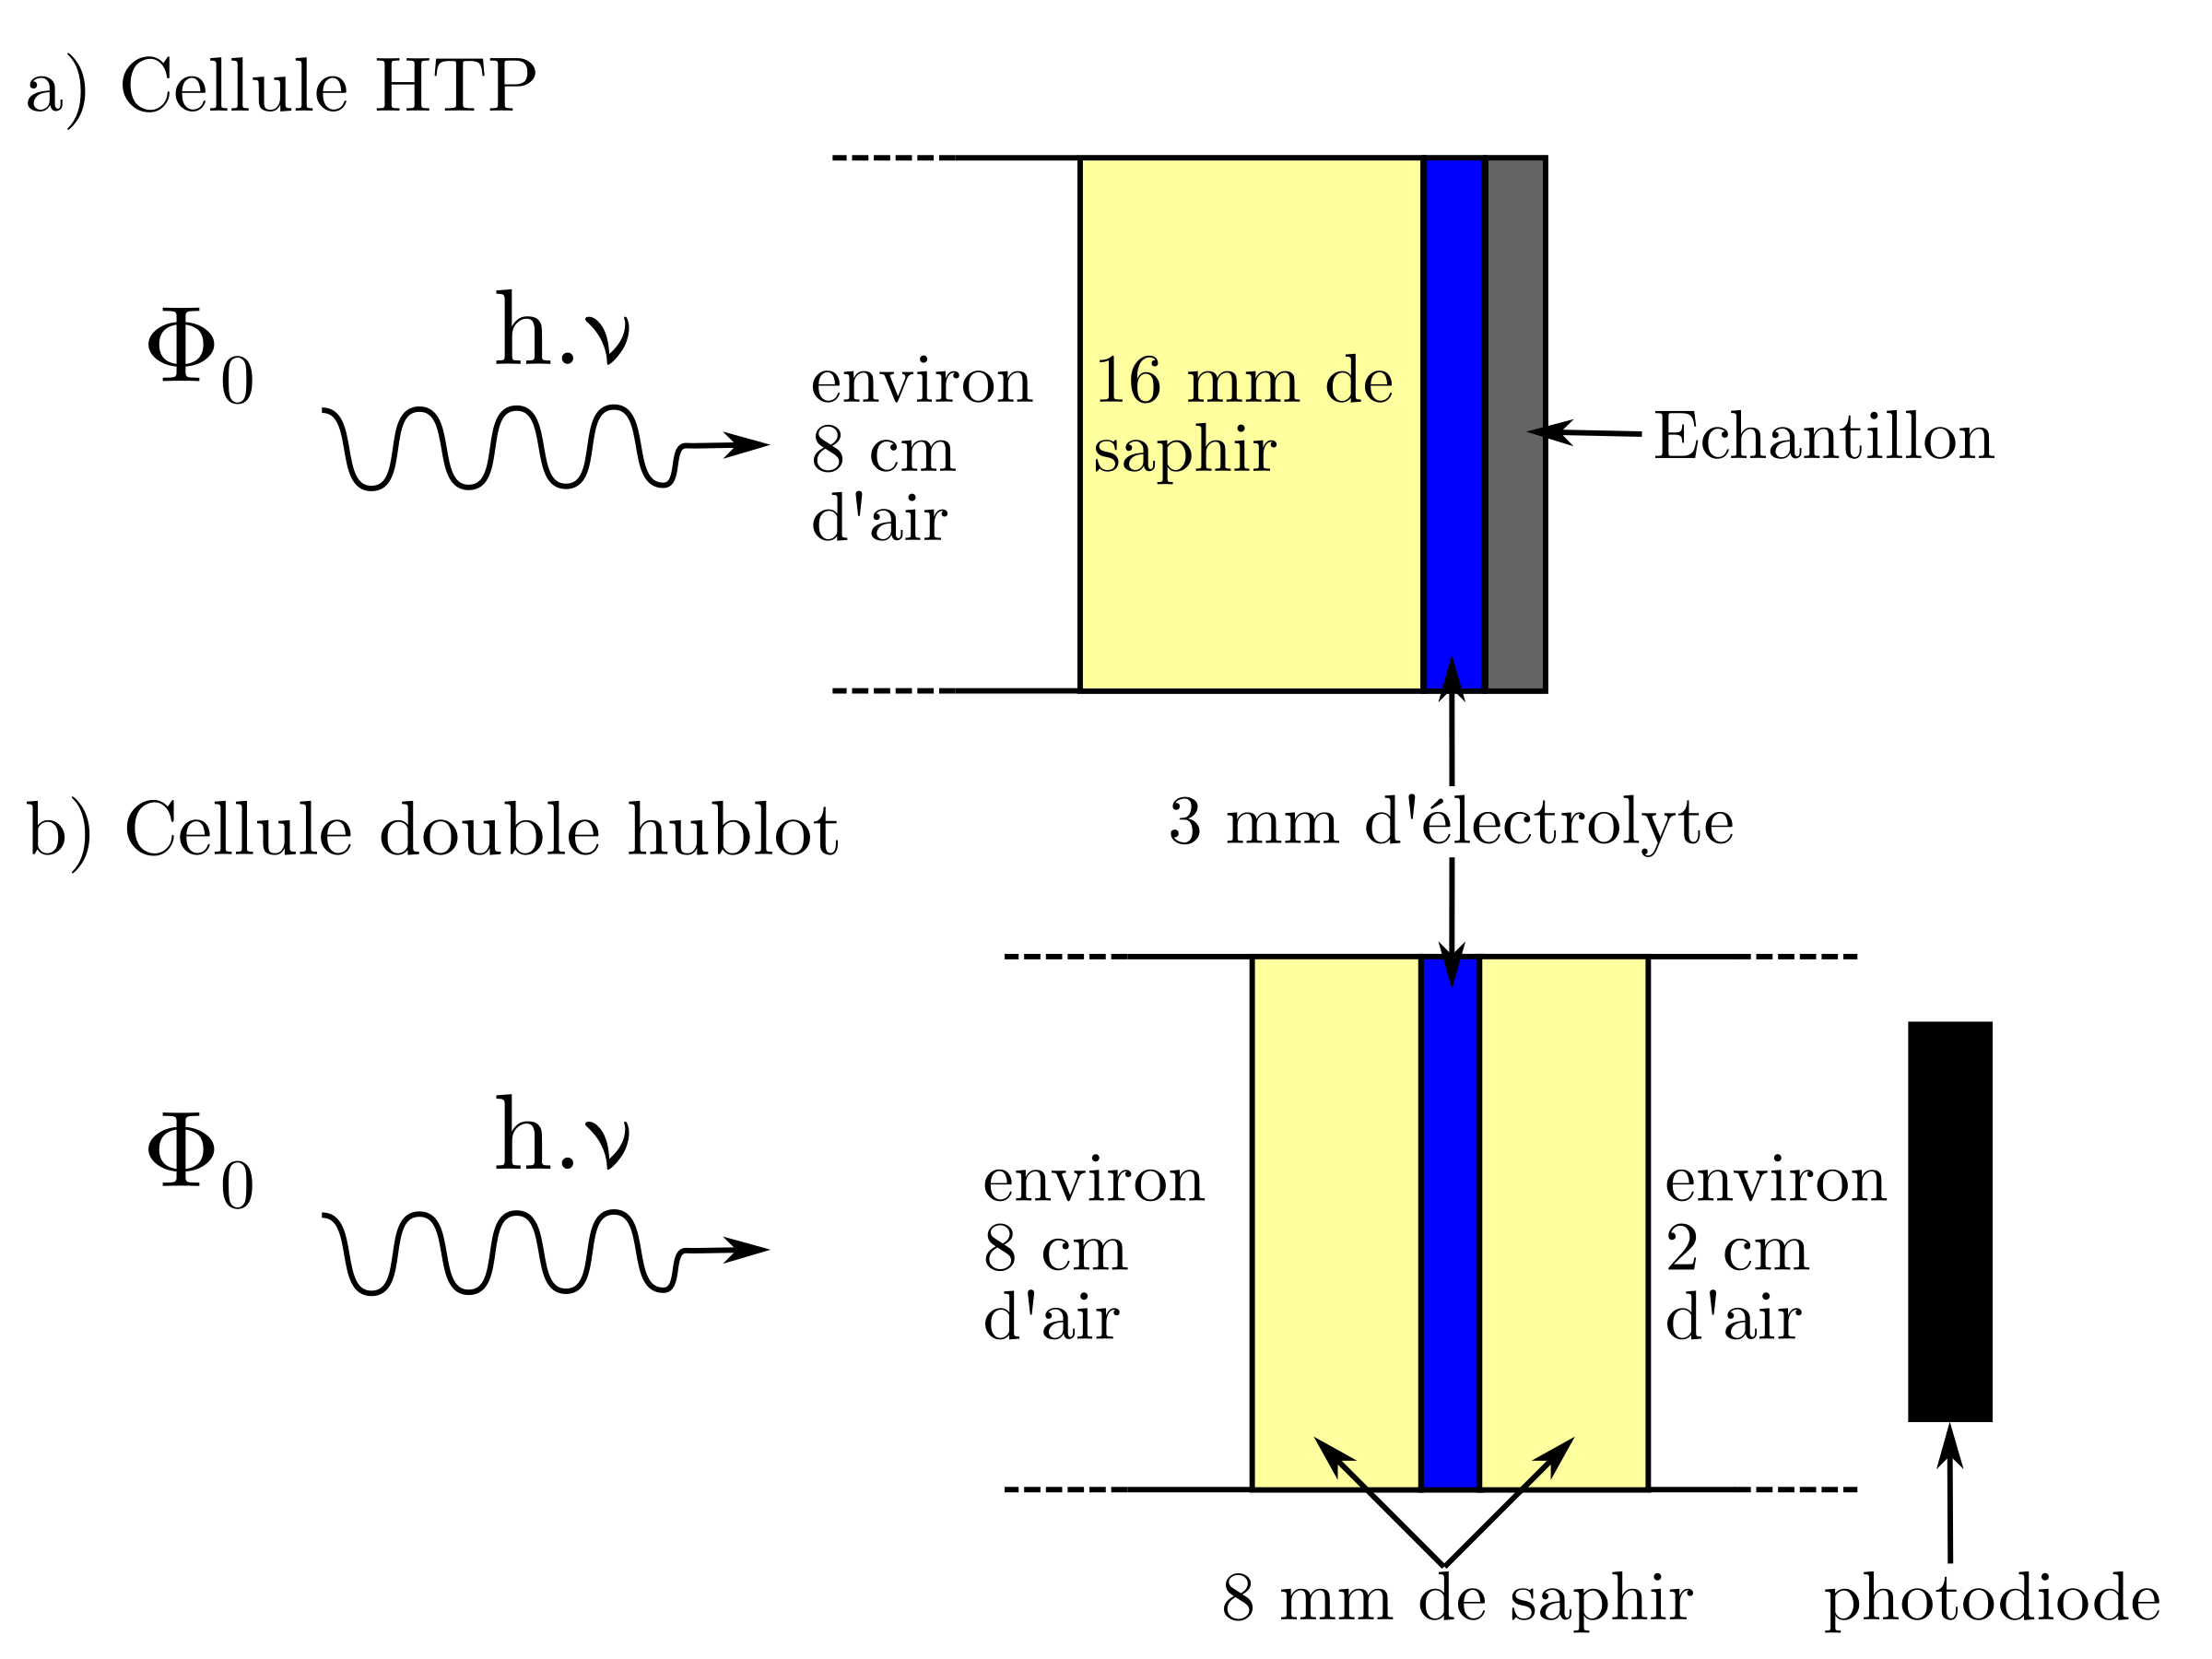
\includegraphics[width=0.85\textwidth]{optical_path.png}
        \caption
        {Chemins optiques du faisceau lumineux incident dans le cas de: 
        a) la cellule HTP,
        b) la cellule double hublot.}
		\label{fig:ch3_optical_paths}
	\end{figure}

    L'illumination à travers la cellule double hublot se fait avec la sortie
    latérale du monochromateur alors que l'illumination des échantillons est faite avec la sortie axiale.
    En toute rigueur, il faudrait utiliser la sortie axiale du monochromateur
    pour mesurer le flux de photons à travers la cellule double hublot, mais l'utilisation de la sortie
    latérale facilite grandement l'alignement du monochromateur avec les cellules (voir \S\ref{sec:complete_experimental_setup}).    
    Par conséquent, les flux de photons mesurés avec la cellule double hublot sont différents des flux de photons
    arrivant à la surface de l'échantillon dans la cellule HTP, mais les flux relatifs aux diverses longueurs d'onde
    restent les mêmes.
    
    La figure \ref{fig:ch3_lamp_spectra_illustration} présente l'allure du spectre de lampe (Xe) mesuré avec la cellule
    double hublot. A titre de comparaison, le spectre mesuré directement sur la sortie latérale du monochromateur est
    également représenté. On constate bien qu'il ne suffit pas de mesurer les flux en sortie de monochromateur pour
    connaître ceux qui atteignent l'échantillon.

     
    \begin{figure}[H]
		\centering
		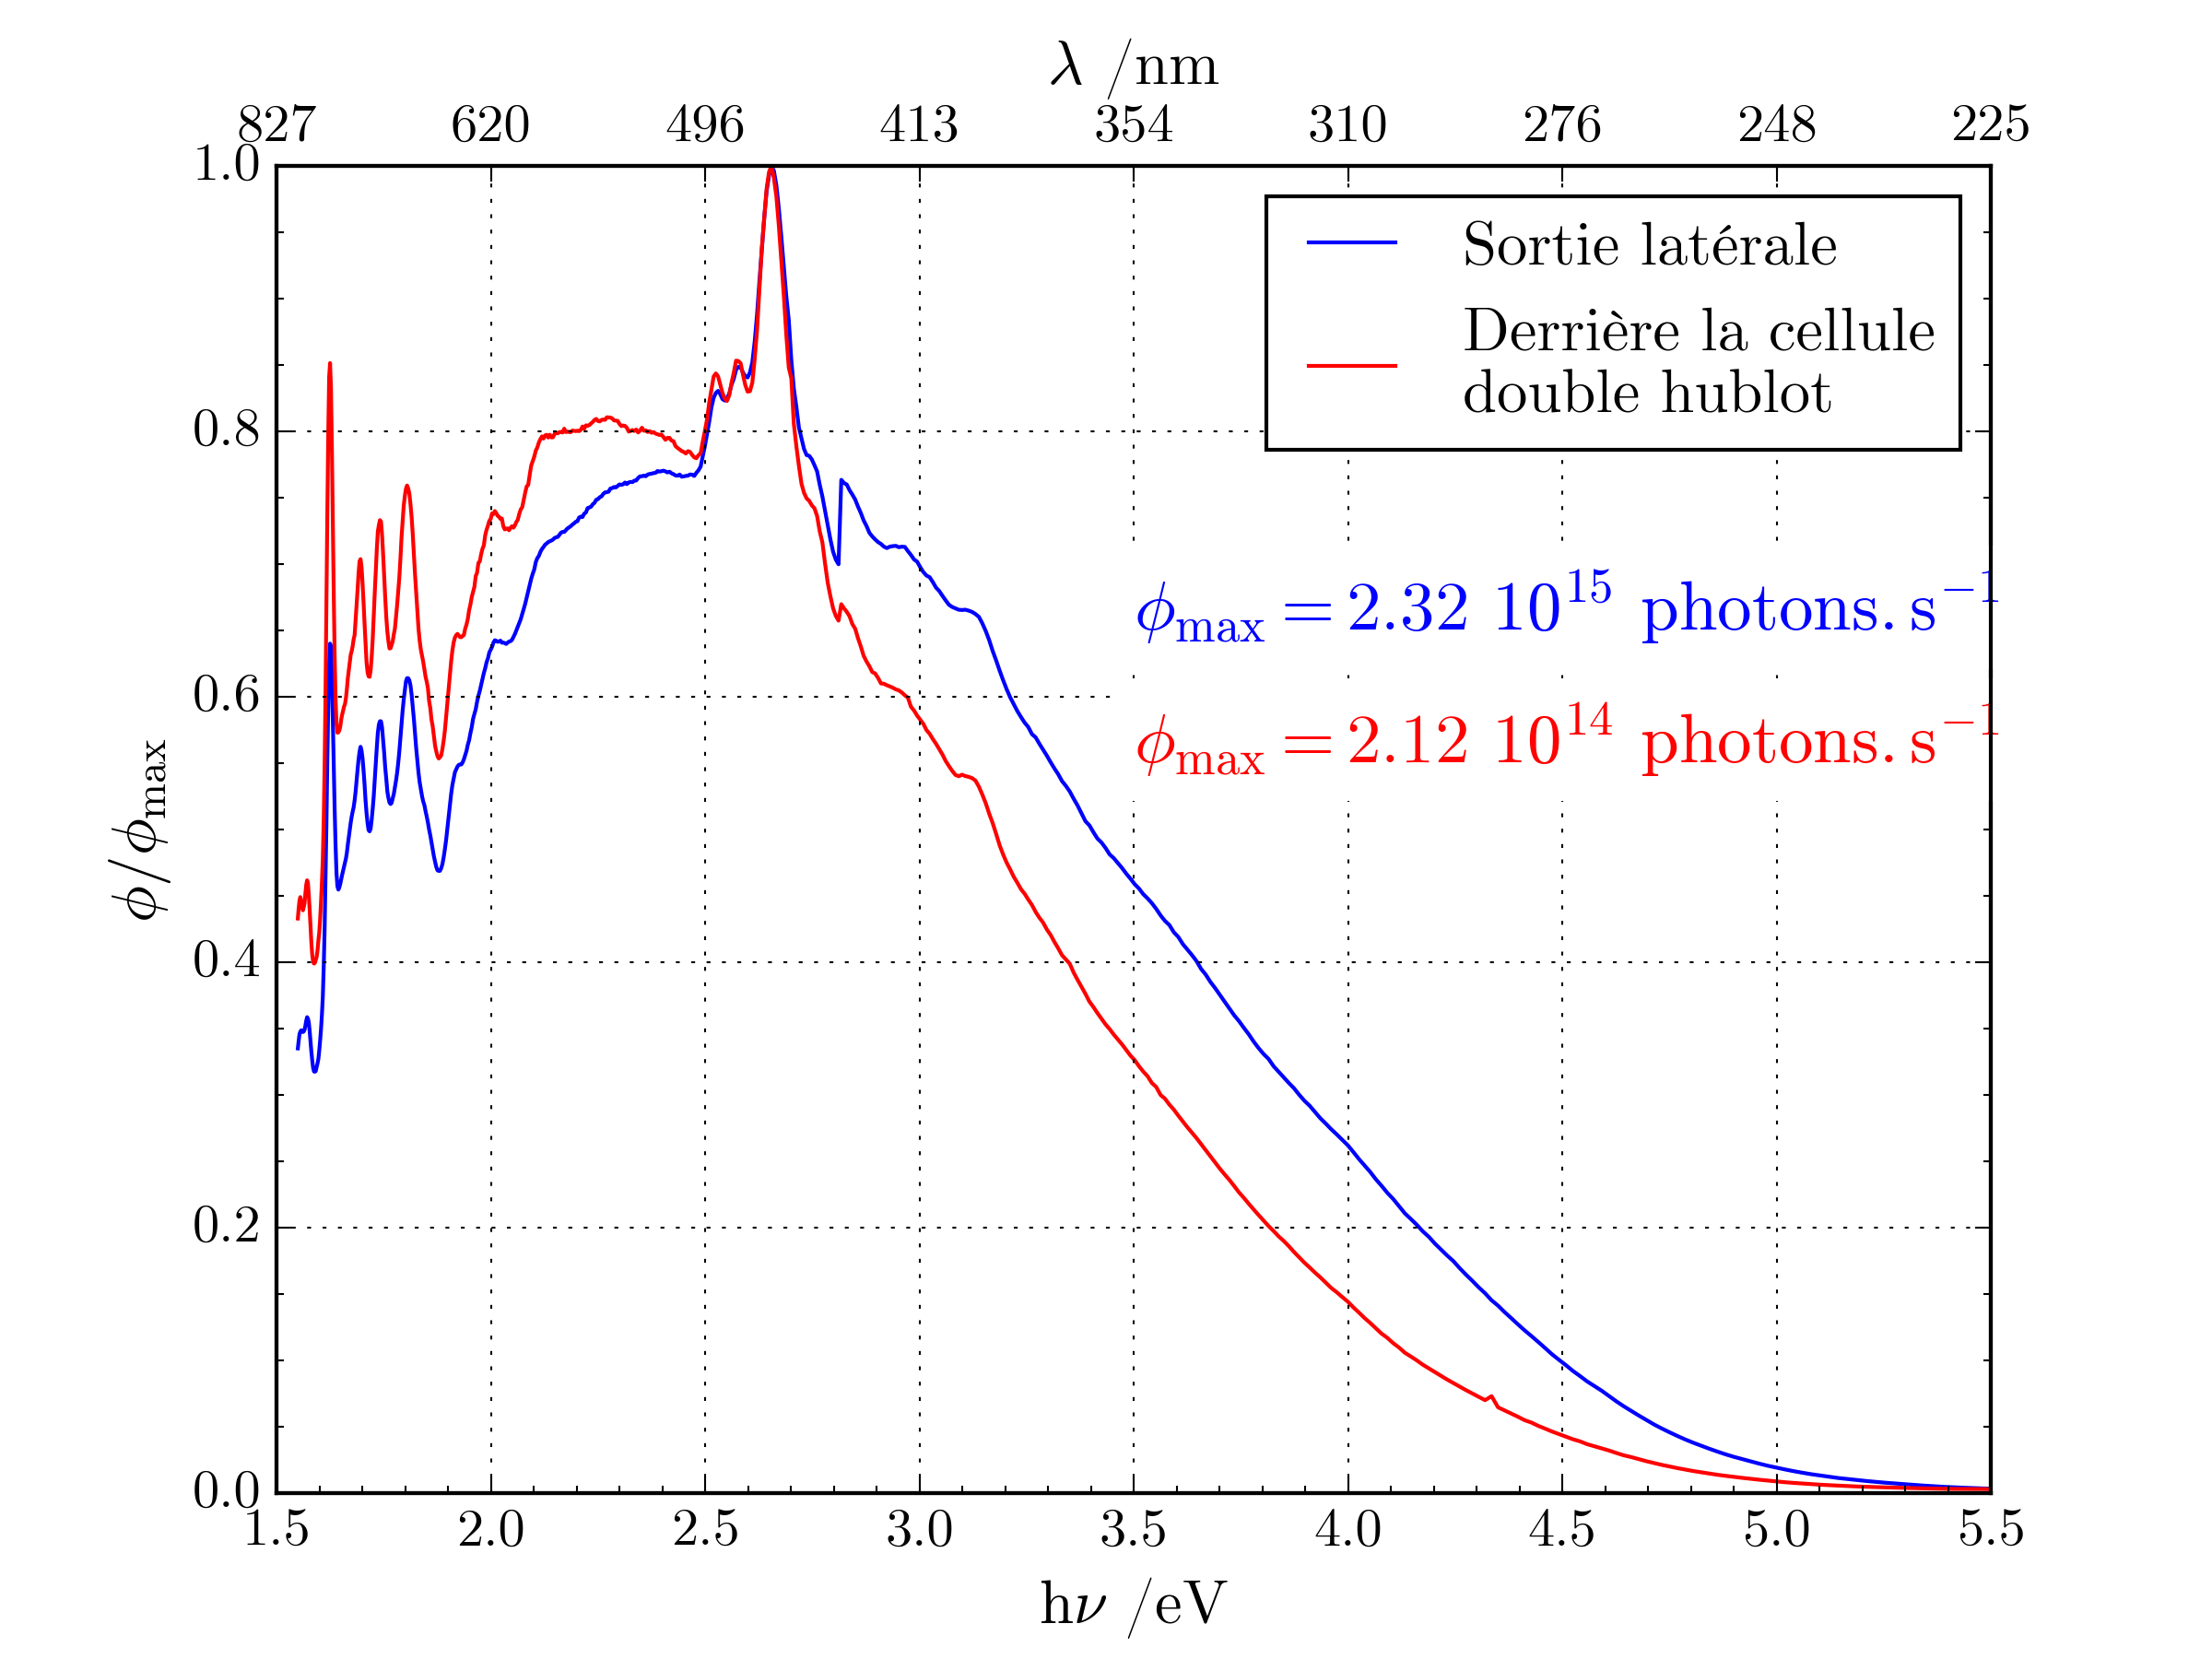
\includegraphics[width=0.85\textwidth]{150215-Illustration-Lamp_Spectra-2W.png}
        \caption
        {"Spectres de lampe" mesurés avec la photodiode placée: 
        a) directement à la sortie latérale du monochromateur,
        b) derrière la cellule double hublot positionnée face à cette sortie latérale.}
		\label{fig:ch3_lamp_spectra_illustration}
	\end{figure}



%%%%%%%%%%%%%%%%%%%%%%%%%%%%%%%%%%%%%%%%%%%%%%%%%%%%%%%%%%%%%%%%%%%%%%%%
\section{Dispositif expérimental complet}\label{sec:complete_experimental_setup}

    La cellule HTP ainsi que la cellule double hublot ont été intégrées sur la boucle de contrôle de la chimie
    PIERE (\textbf{P}lateforme \textbf{I}ntégrée pour l'\textbf{E}tude du \textbf{R}elâchement et de 
    l'oxydation en milieu primaire) mise à notre
    disposition par le Centre Technique d'Areva au Creusot mais qui a dû être rénovée pour l'occasion.
    La figure \ref{fig:complete_experimental_setup} présente de manière schématique le dispositif expérimental complet.
    Le logiciel de pilotage de la boucle est un logiciel
    développé en interne au Centre Technique du Creusot, également remis à jour dans le cadre de notre travail.
    L'ensemble des capteurs disponibles sur la boucle ont également été étalonnés.

    Les connections entre les différents éléments sont réalisées avec du tube \emph{Swagelock 6.35} en inox 316L. 
    La mise en pression de tout le circuit est assurée par une pompe fourni par \emph{Lewa}. La circulation se fait en
    \emph{one-through} c'est-à-dire que l'électrolyte n'est pas recyclé.   

    \begin{figure}[H]
        \centering
        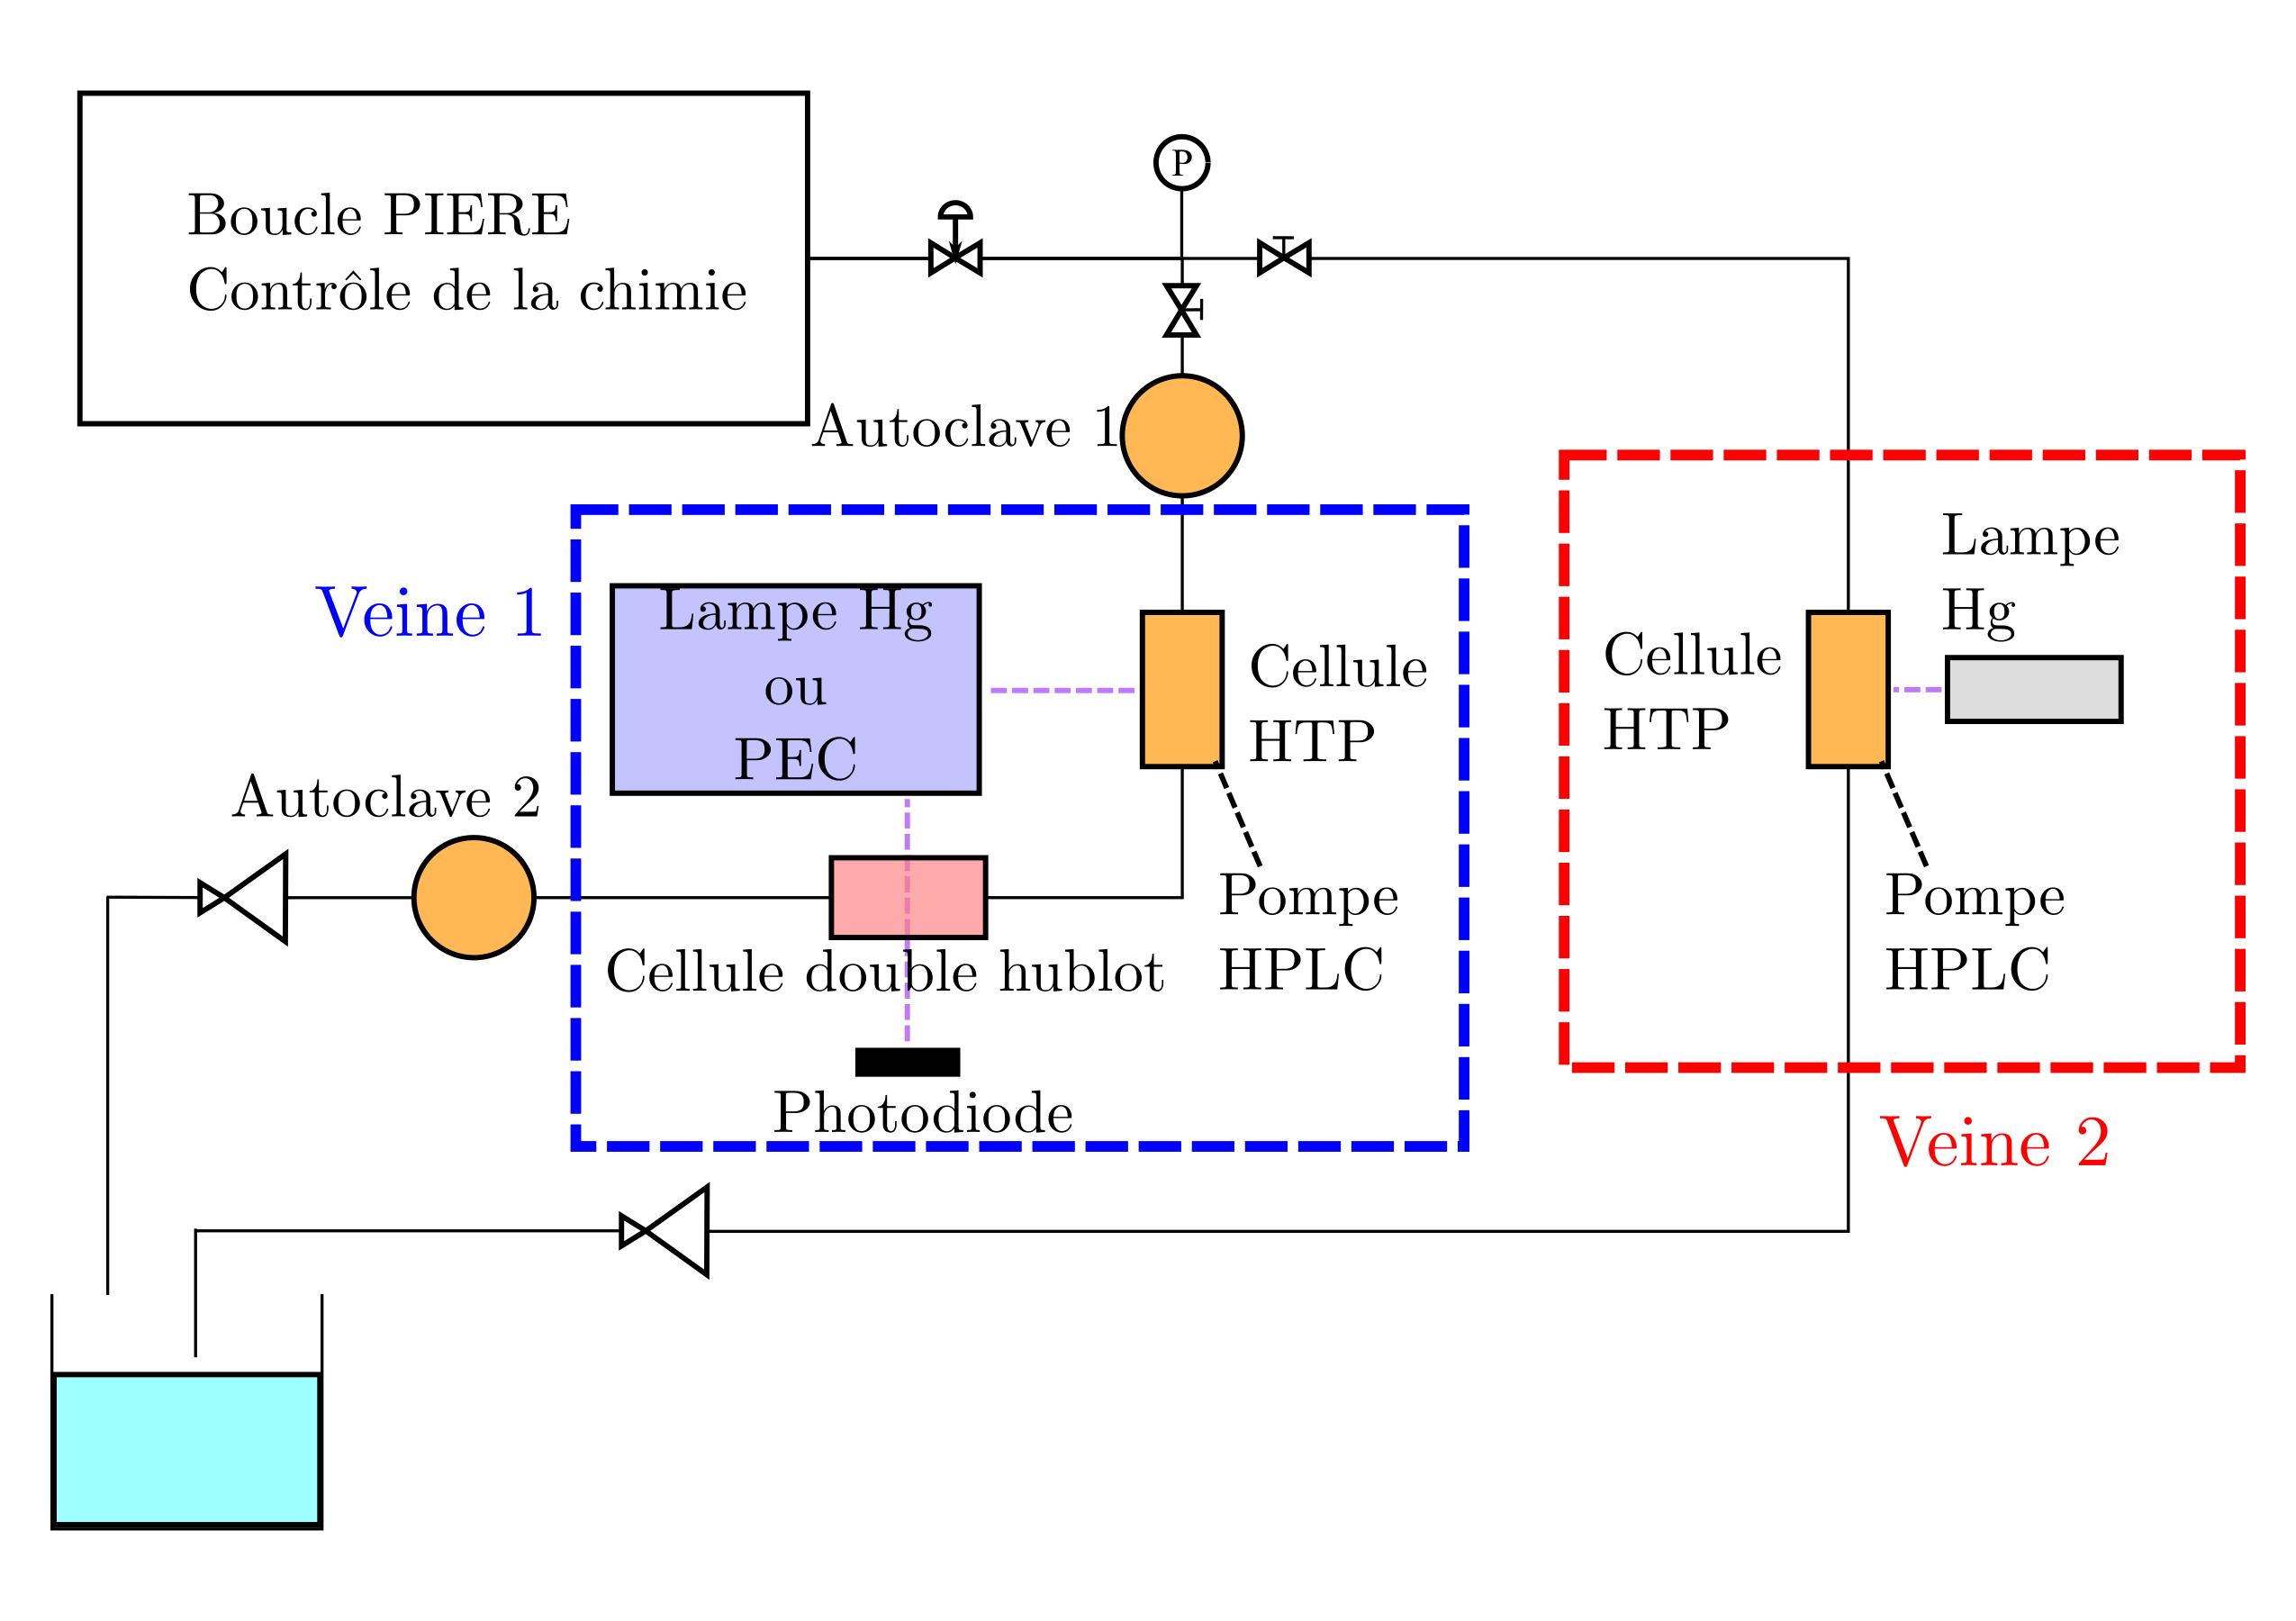
\includegraphics[width=0.95\textwidth]{Experimental_Setup-2-new.png}
        \caption{Représentation schématique de l'ensemble du dispositif expérimental incluant la boucle PIERE, la
        cellule HTP et la cellule double hublot.}
        \label{fig:complete_experimental_setup}
    \end{figure}
    %\ref{chap:ch4_results}
    Initialement deux veines de circulation ont été prévues afin de pouvoir
    réaliser des caractérisations PEC (veine 1) et des illuminations intenses de longue durée (veine 2). Cependant, la gestion de la température sur
    les deux veines, fonctionnant simultanément, s'est révélée être plus difficile que prévu. 
    Afin de ne pas ralentir la réalisation des
    premiers essais, la deuxième veine n'a pas été utilisée et l'ensemble des résultats présentés
    au chapitre 4 a été obtenu sur la veine 1. Pour les mêmes raisons de gestion de la
    thermique, les autoclaves de la veine 1, placés en amont et en aval de la cellule HTP, n'ont pas été
    utilisés. La régulation du débit dans la veine est assuré par un débitmètre massique \emph{Liquid-Flow} 
    fourni par \emph{Bronkhorst}.
    Pour minimiser les difficultés de gestion de la température, le débit a été fixé à
    \SI{1}{\milli\liter\per\minute}. Cela correspond à une vitesse d'écoulement moyenne d'environ
    \SI{1.5}{\milli\meter\per\second} dans du tube \emph{Saweglock 6.35} et cette vitesse est encore plus faible dans la
    cellule HTP car la section de passage est plus importante. Mais l'imposition d'un débit était simplement destinée
    à rafraîchir l'électrolyte au niveau de l'échantillon, et non pour étudier l'impact du transport d'électrolyte.

    Comme déjà mentionné au paragraphe \ref{sec:2W_cell}, la sortie axiale du monochromateur est utilisée pour
    illuminer les échantillons alors que la sortie latérale est utilisée pour estimer le flux
    de photons. Le basculement entre les deux sorties se fait à l'aide d'un miroir motorisé situé dans le monochromateur.
    En faisant le choix de travailler avec les deux sorties, cela permet de fixer la position du
    monochromateur de manière à ce que la cellule HTP ainsi que la cellule double hublot soient alignées
    avec les sorties axiale et latérale, respectivement, sans qu'il soit nécessaire de déplacer
    l'ensemble lampe+monochromateur.   
    L'alignement de la lampe Hg était plus simple puisque celle-ci est équipée d'une fibre optique de longueur
    \SI{1}{\meter}, alignée manuellement avec un support en téflon et placée au plus près du
    hublot de saphir. 
    La figure \ref{fig:ch3_sources_alignment} illustre le positionnement des deux sources d'illumination.
      
    \begin{figure}[H]
        \centering
        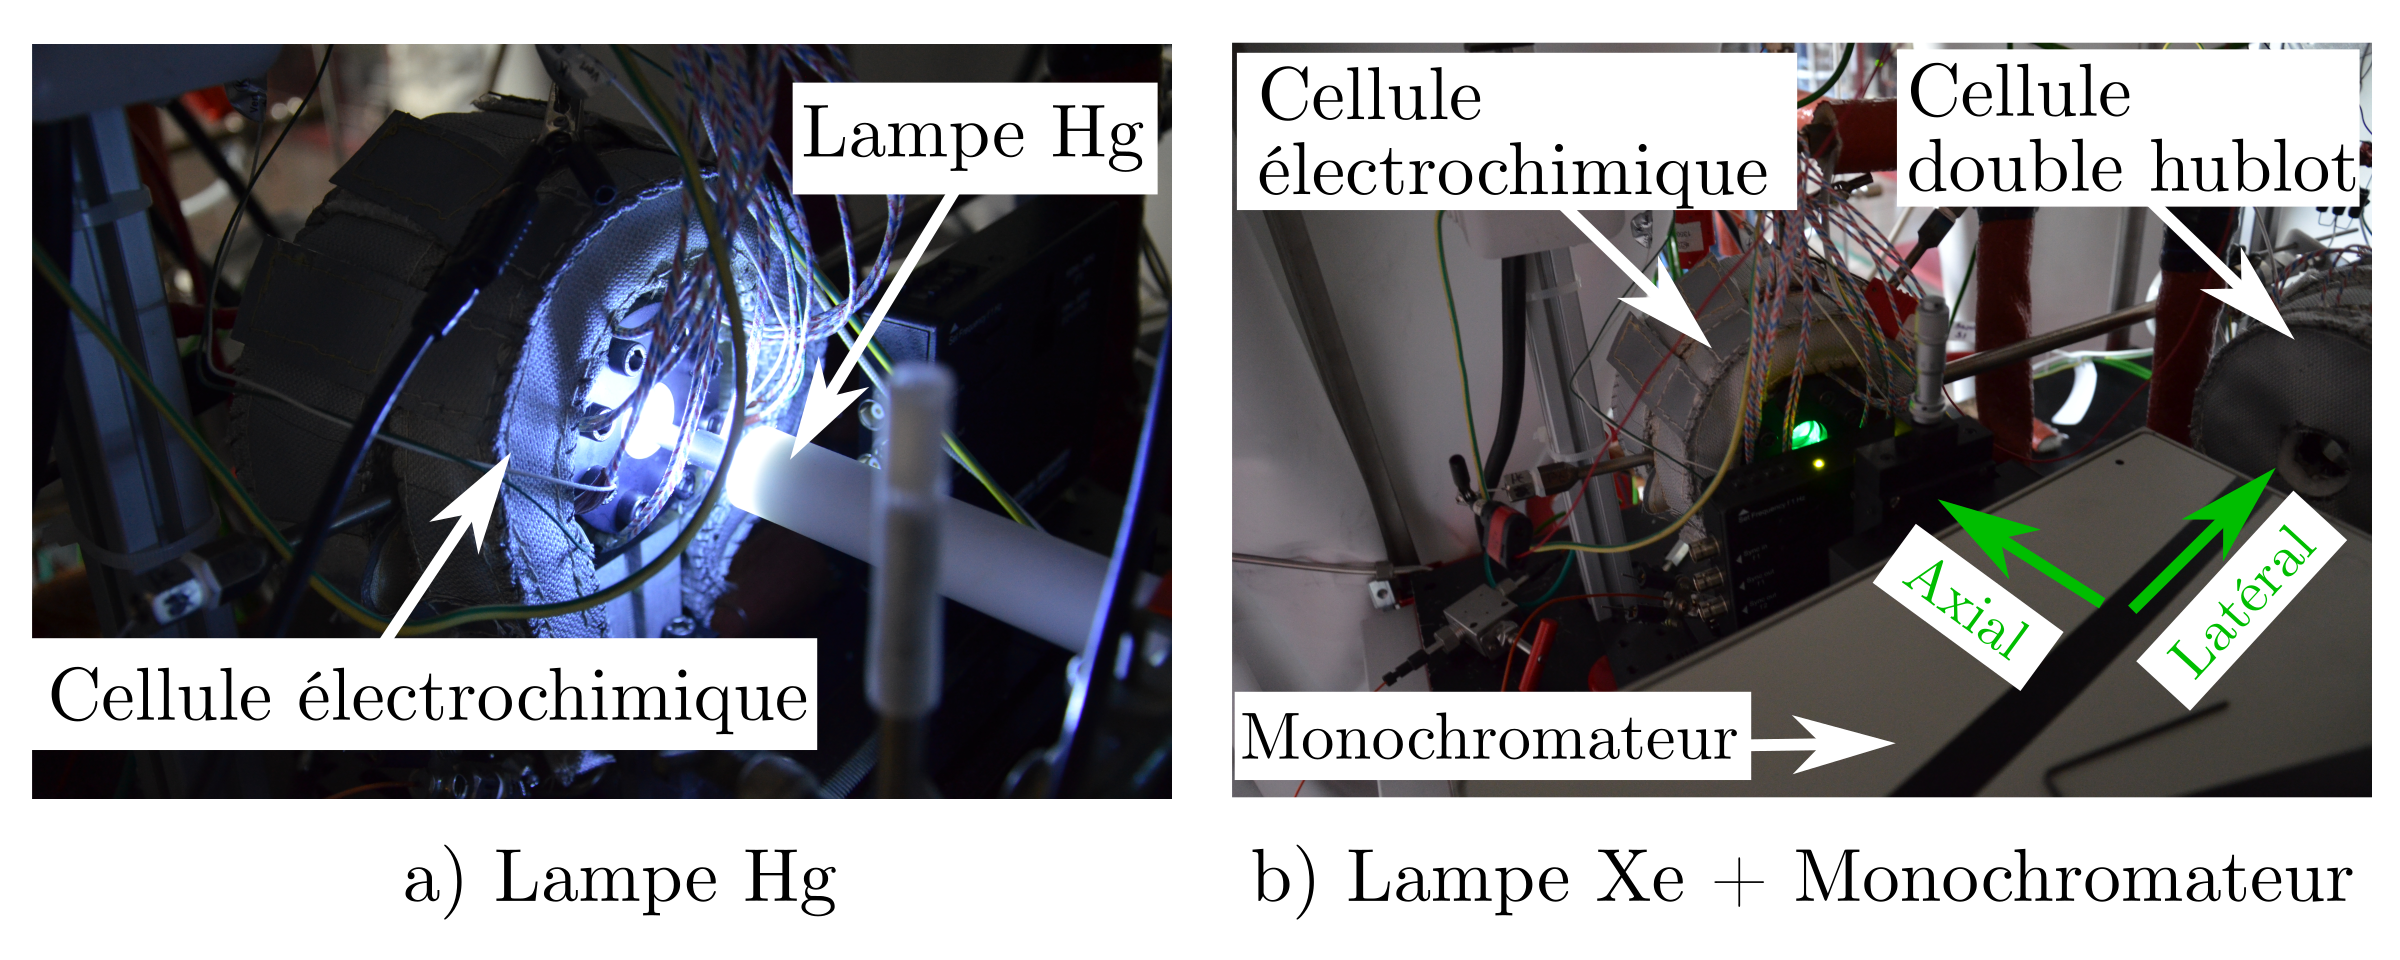
\includegraphics[width=0.95\textwidth]{141059-Illuminations.png}
        \caption{Positionnement et alignement des deux sources d'illumination.}
        \label{fig:ch3_sources_alignment}
    \end{figure}

    %\subsection{Contrôle de la température}\label{subsec:ch3_temperature_management}
    Le maintien de la température des deux cellules est assuré par des cartouches chauffantes directement positionnées
    dans les corps de cellule (voir \S\ref{sec:ch3_cell} et \S\ref{sec:2W_cell}).
    La préchauffe de l'électrolyte en amont des deux cellules est assurée par des tresses
    chauffantes.
    Tous les éléments chauffants sont pilotés par des régulateurs \emph{Eurotherm 2208e}. La régulation est
    effectuée avec des thermocouples K en contact avec l'électrolyte dans les deux cellules ainsi que dans la veine en amont des
    cellules (environ \SI{5}{\centi\meter}).
    Le réglage du PID des cartouches chauffantes est relativement simple grâce à l'inertie thermique du corps de
    cellule. Ce n'est pas le cas pour les tresses chauffantes qui sont enroulées autour des
    tubes de circulation qui ont peu d'inertie thermique. Une solution temporaire a été de fixer sur les régulateur PID
    le paramètre proportionnel
    et de désactiver les paramètres intégrale et dérivée. 
    %Finalement, seul le temps de chauffe par cycle de régulation
    %est modifié afin d'atteindre la température désirée. 
    
    La figure \ref{fig:ch3_temperature_management} présente les
    profils de température mesurés dans les deux cellules et en amont de celle-ci. La température est maintenue à
    $281 \pm 2 \si{\degreeCelsius}$ dans la cellule HTP alors que la température en amont de celle-ci oscille fortement autour
    de \SI{260}{\degreeCelsius}. Les mêmes oscillations ont été observées en amont de la cellule double hublot. De plus, la
    température maximale atteinte dans la cellule double hublot est seulement de $235 \pm 1 \si{\degreeCelsius}$ très
    probablement en raison de la présence des deux hublots qui entraînent une forte déperdition thermique.
    
    \begin{figure}[H]
        \centering
        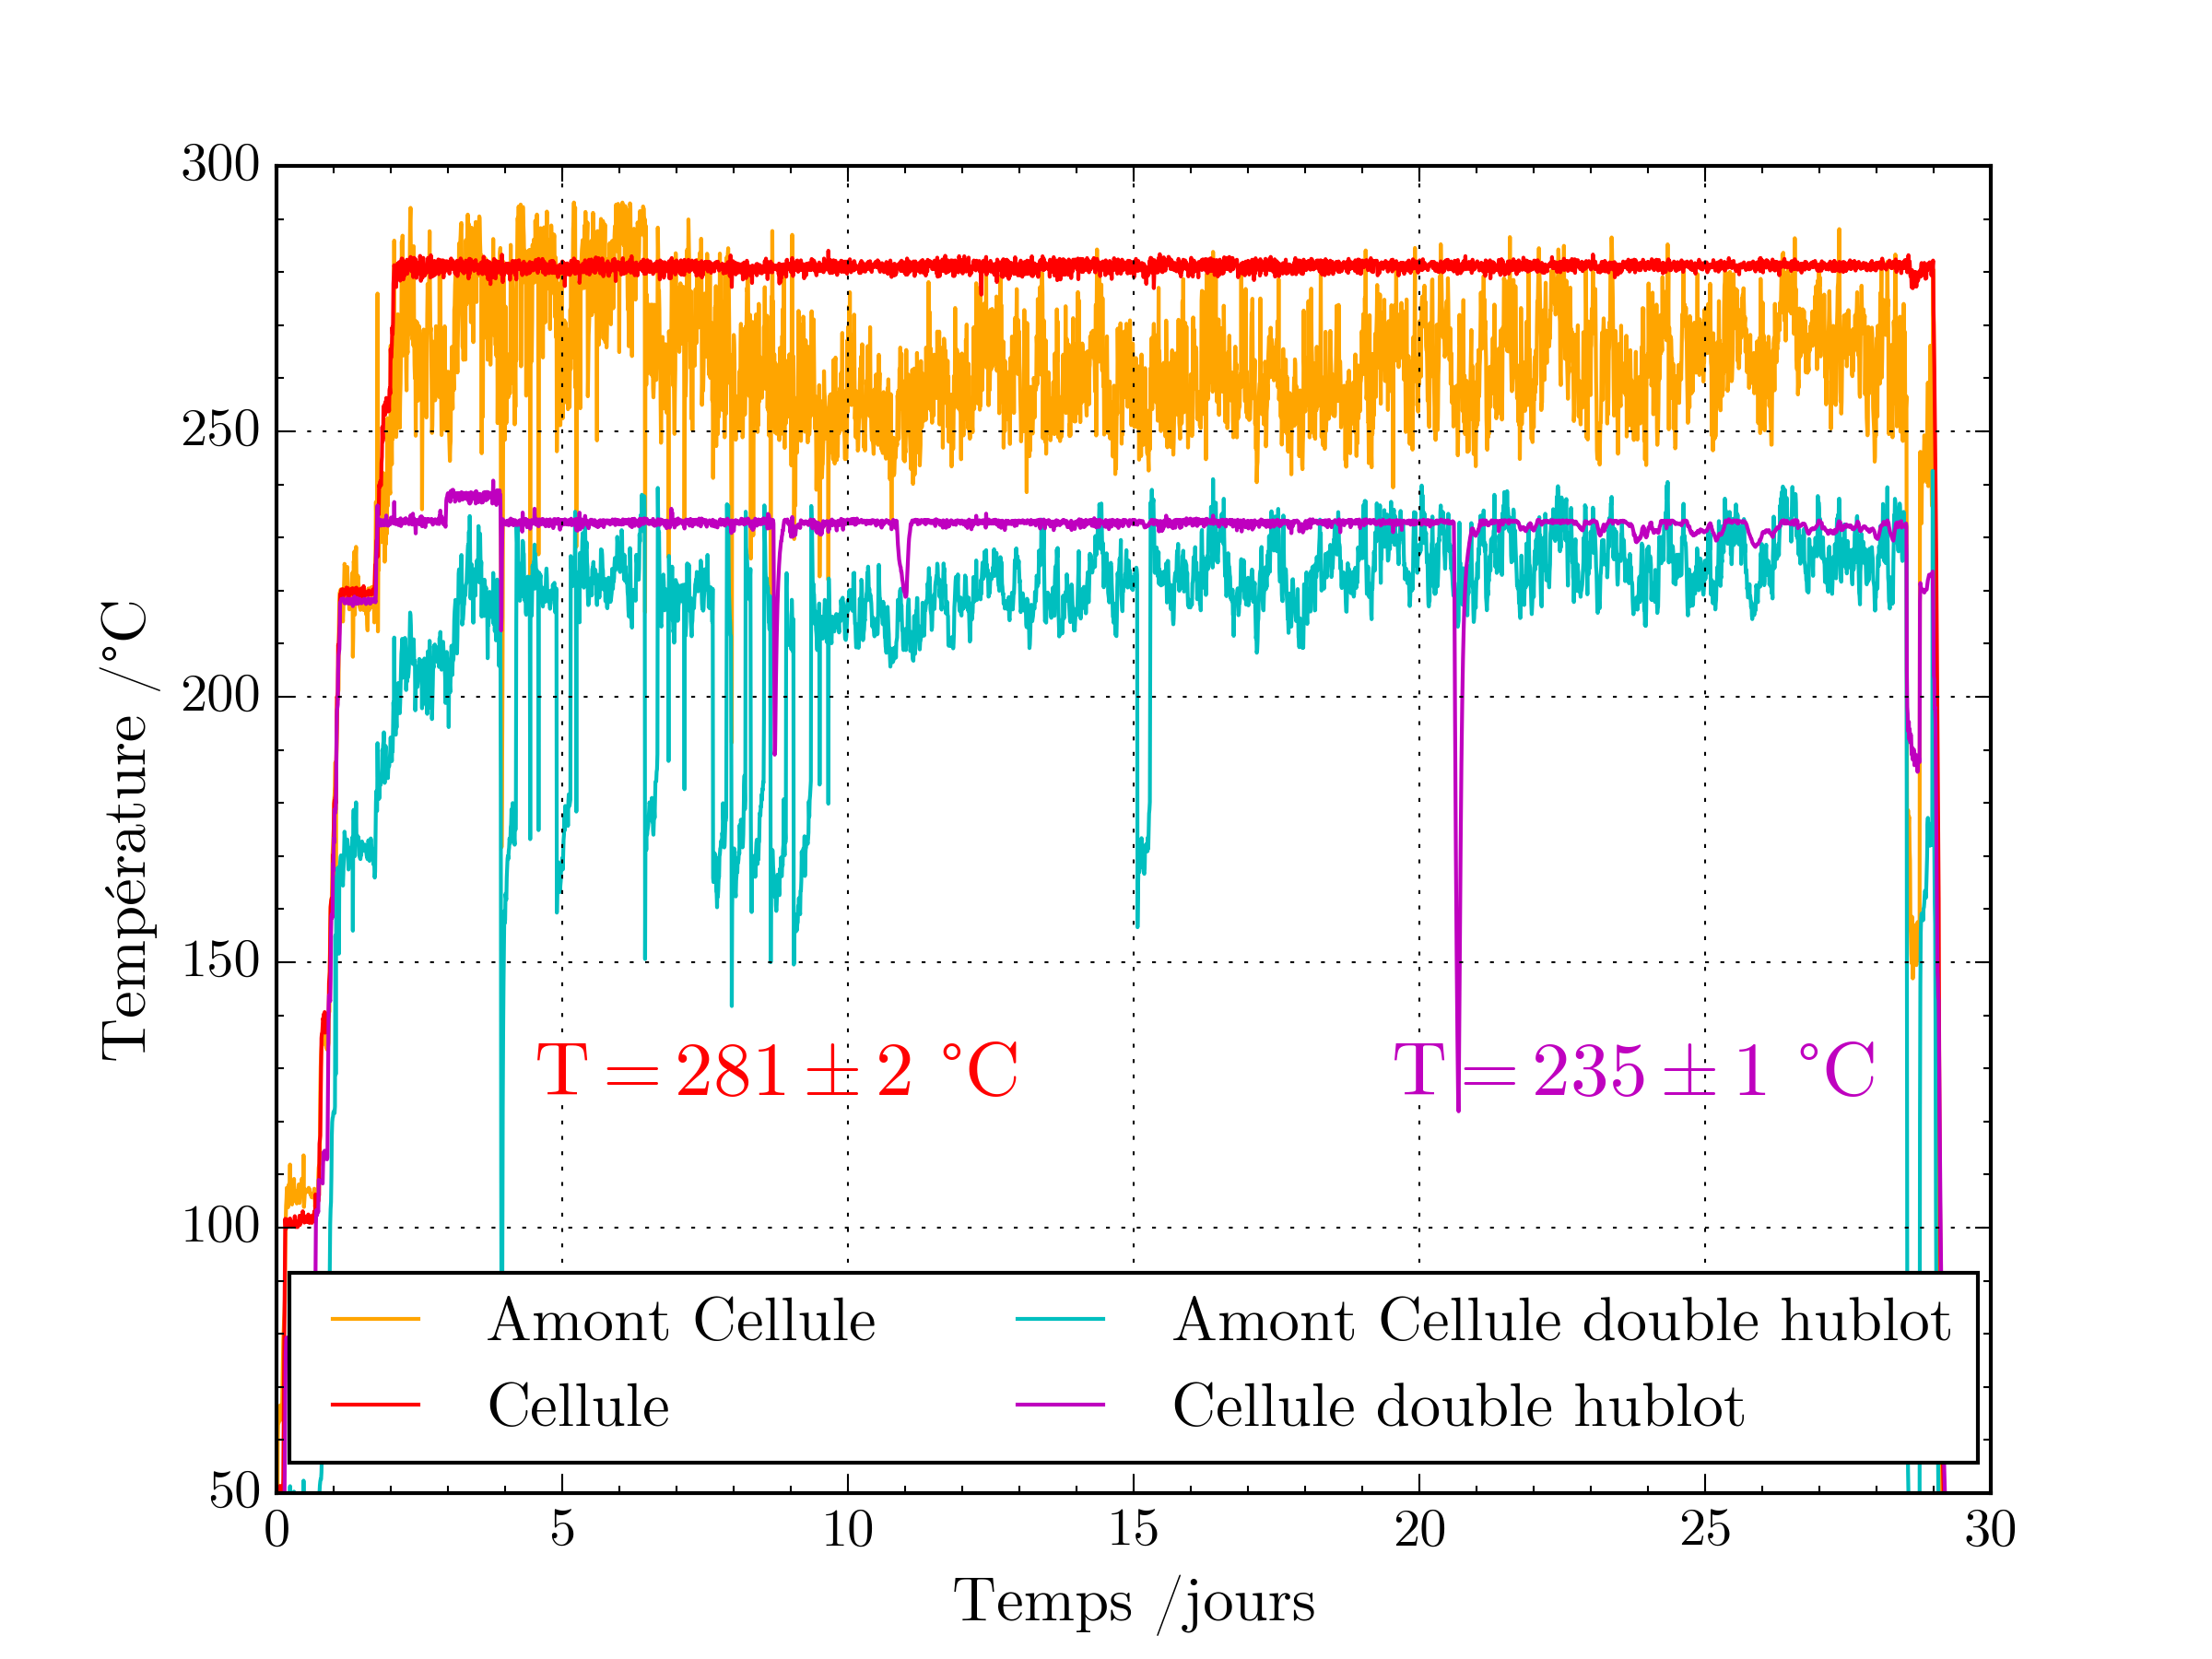
\includegraphics[width=0.65\textwidth]{150215-Illustration-Temperature-All.png}
        \caption{Profils de température en amont des deux cellules et dans les deux cellules.}
        \label{fig:ch3_temperature_management}
    \end{figure}


    %\subsection{Contrôle de la teneur en oxygène et peroxyde d'hydrogène}\label{subsec:ch3_O2_H2O2_management}
    La teneur en oxygène dissous dans l'électrolyte (eau ultra-pure) a été ajustée par bullage d'un mélange d'argon et
    d'oxygène dans une bâche de \SI{50}{\liter} dans la partie basse pression de la boucle qui se trouve à
    température ambiante. D'un point de vue expérimental, le mélange est réalisé avec une
    bouteille d'argon pur et une bouteille d'un mélange argon/oxygène à \SI{1}{\percent} d'oxygène fournies par
    \emph{Westfallen}. Le taux de dissolution théorique est d'abord calculé en tenant compte de la surpression dans la bâche et
    de la constante de dissolution de l'oxygène \citep{Tromans1998}. Ce taux de dissolution est ensuite utilisé pour
    régler des débitmètres gaz \emph{Smart Mass Flow} fourni par \emph{Brooks}. La teneur réelle en oxygène dissous est mesurée avec un
    orbisphère \emph{HACH 410} équipé d'une membrane \emph{2956A}, étalonné à chaque changement de membrane. Les
    débits sont éventuellement réajustés par rapport aux valeurs théoriques afin d'atteindre la valeur désirée en
    oxygène dissous. La figure \ref{fig:ch3_O2_management} montre l'évolution de la teneur en oxygène en condition
    désaérée et pour une teneur visée de \SI{200}{\ppb}.
    Cette teneur en oxygène a pu généralement être contrôlée à $\pm$ \SI{10}{\ppb} pour des valeurs visées supérieures à
    \SI{50}{\ppb}. 

    La teneur en peroxyde d'hydrogène a été ajustée par injection directe à l'entrée de la cellule HTP.
    L'injection se fait avec une pompe HPLC \emph{Eldex} à travers un capillaire en PEEK. La figure
    \ref{fig:ch3_PEEK_capillary} montre la position du passage étanche utilisé pour l'injection. Le contrôle de la
    teneur obtenue est réalisé en faisant varier le débit d'injection fixant ainsi le taux de dissolution. Cependant, le
    débit d'injection ne doit pas dépasser environ \SI{20}{\percent} du débit de circulation pour ne pas perturber
    la température dans la cellule HTP. En fonction, des teneurs désirées, une solution mère de peroxyde
    d'hydrogène est préparée avec une concentration adéquate. Les débits d'injection utilisés se trouvent dans la
    partie basse de la gamme de travail de la pompe HPLC dont l'erreur sur le débit peut atteindre \SI{10}{\percent}.
    Par conséquent, les teneurs en peroxyde d'hydrogène injectées seront données avec une précision de \SI{10}{\percent}.

    \begin{figure}[H]
        \centering
        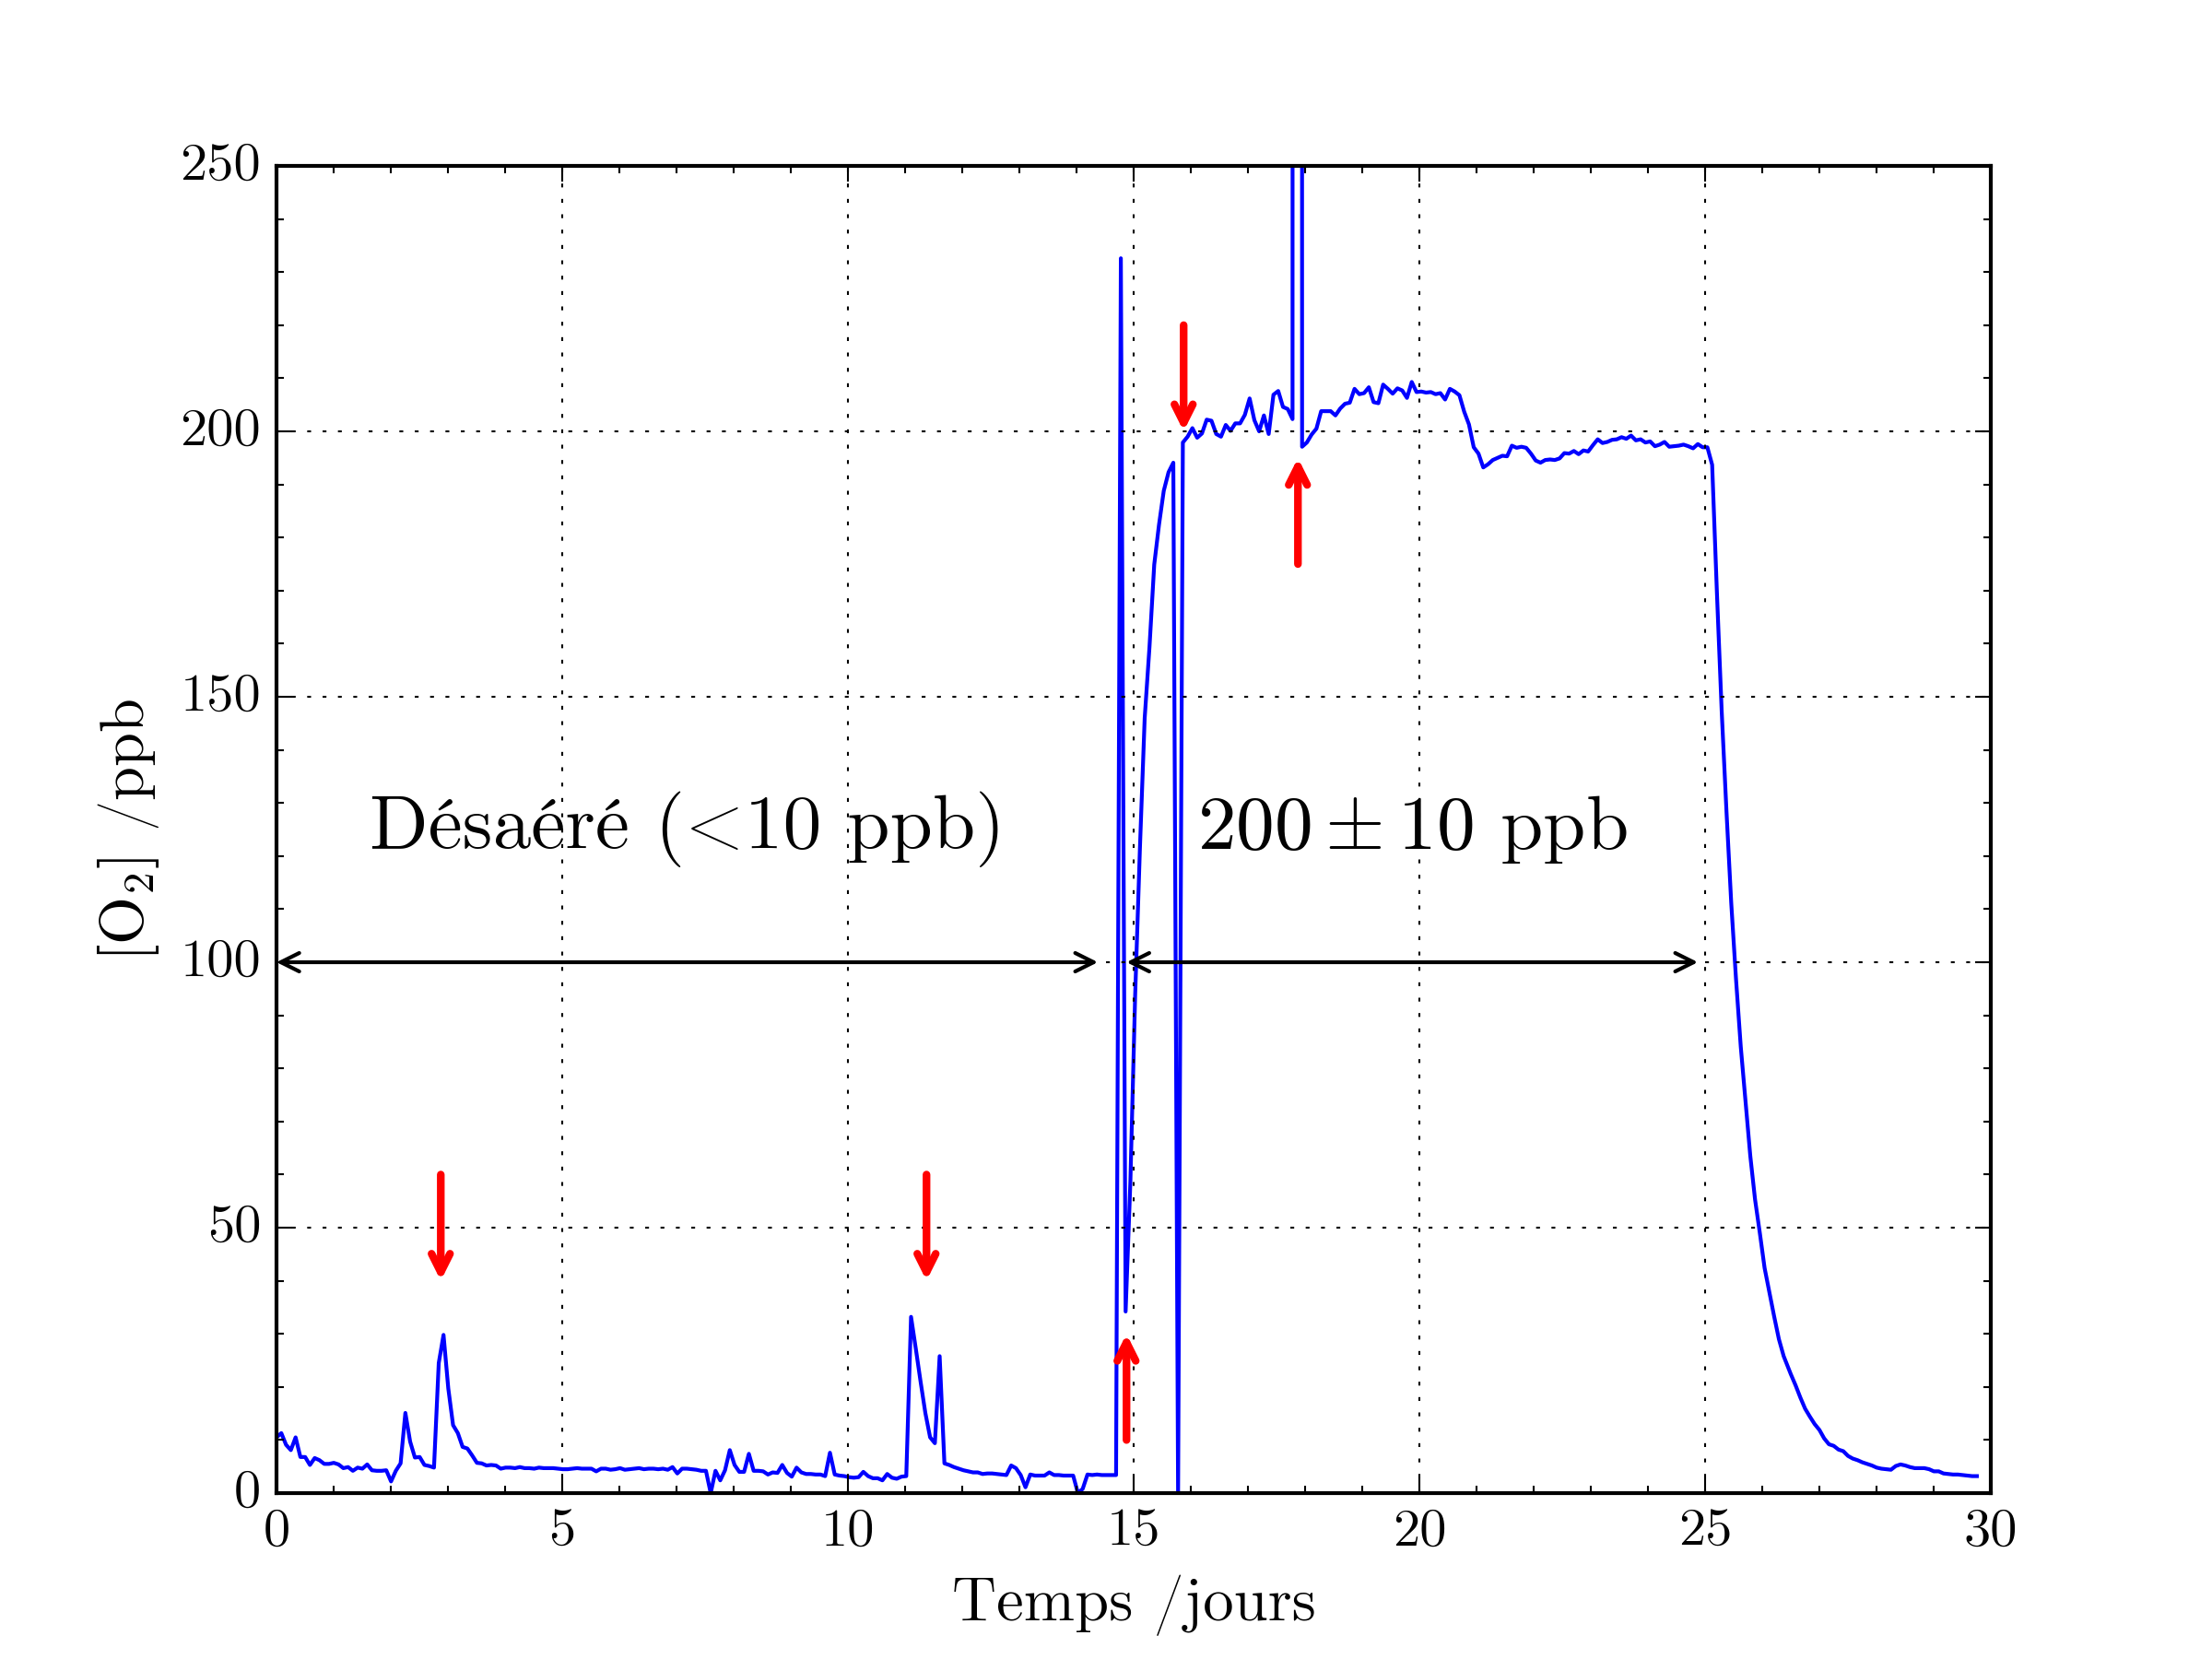
\includegraphics[width=0.65\textwidth]{150215-Illustration-O2-All.png}
        \caption{Profil de la teneur en oxygène dissous mesuré à température ambiante dans la partie basse pression de
        la boucle. Les flèches rouges correspondantent à des défaillances de la communication entre l'ordinateur
    d'acquisition des données et l'orbisphère.}
        \label{fig:ch3_O2_management}
    \end{figure}

    \begin{figure}[H]
        \centering
        \includegraphics[width=0.65\textwidth]{141059-PEEK_Capillary.png}
        \caption{Passage étanche pour l'injection de peroxyde d'hydrogène à l'entrée de la cellule HTP.}
        \label{fig:ch3_PEEK_capillary}
    \end{figure}

\section{Conclusions}\label{sec:ch3_conclusion}

    Malgré de très nombreux aléas et difficultés techniques rencontrés, le développement du dispositif expérimental
    a pu être mené à bien. Avant de présenter et discuter nos résultats, nous donnons ci-dessous quelques exemples
    d'expériences que nous avons pu réaliser avec notre dispositif.
    Ainsi la cellule HTP permet de
    suivre l'évolution du potentiel libre et du courant de couplage avec et sans illumination UV--Visible intense par la lampe
    Hg comme dans les travaux de \citet{Kim2010} (ch.\ref{chap:ch1_bib} \S\ref{sec:out_of_pile_experiments}). La
    figure \ref{fig:ch3_illustration_ECP} présente la diminution du potentiel libre des alliages Zy2 et Inc718 sous
    illumination UV--Visible, traduisant un comportement semiconducteur de type \emph{n} pour les deux échantillons. L'augmentation de la différence de
    potentiel sous illumination UV--Visible intense se traduit par courant supplémentaire lorsque ces deux alliages sont en situation de
    couplage  comme illustré par la figure \ref{fig:ch3_illustration_ZRA} qui présentent des résultats de mesure par ZRA
    dans notre cellule HTP.

    \begin{figure}[H]
        \centering
            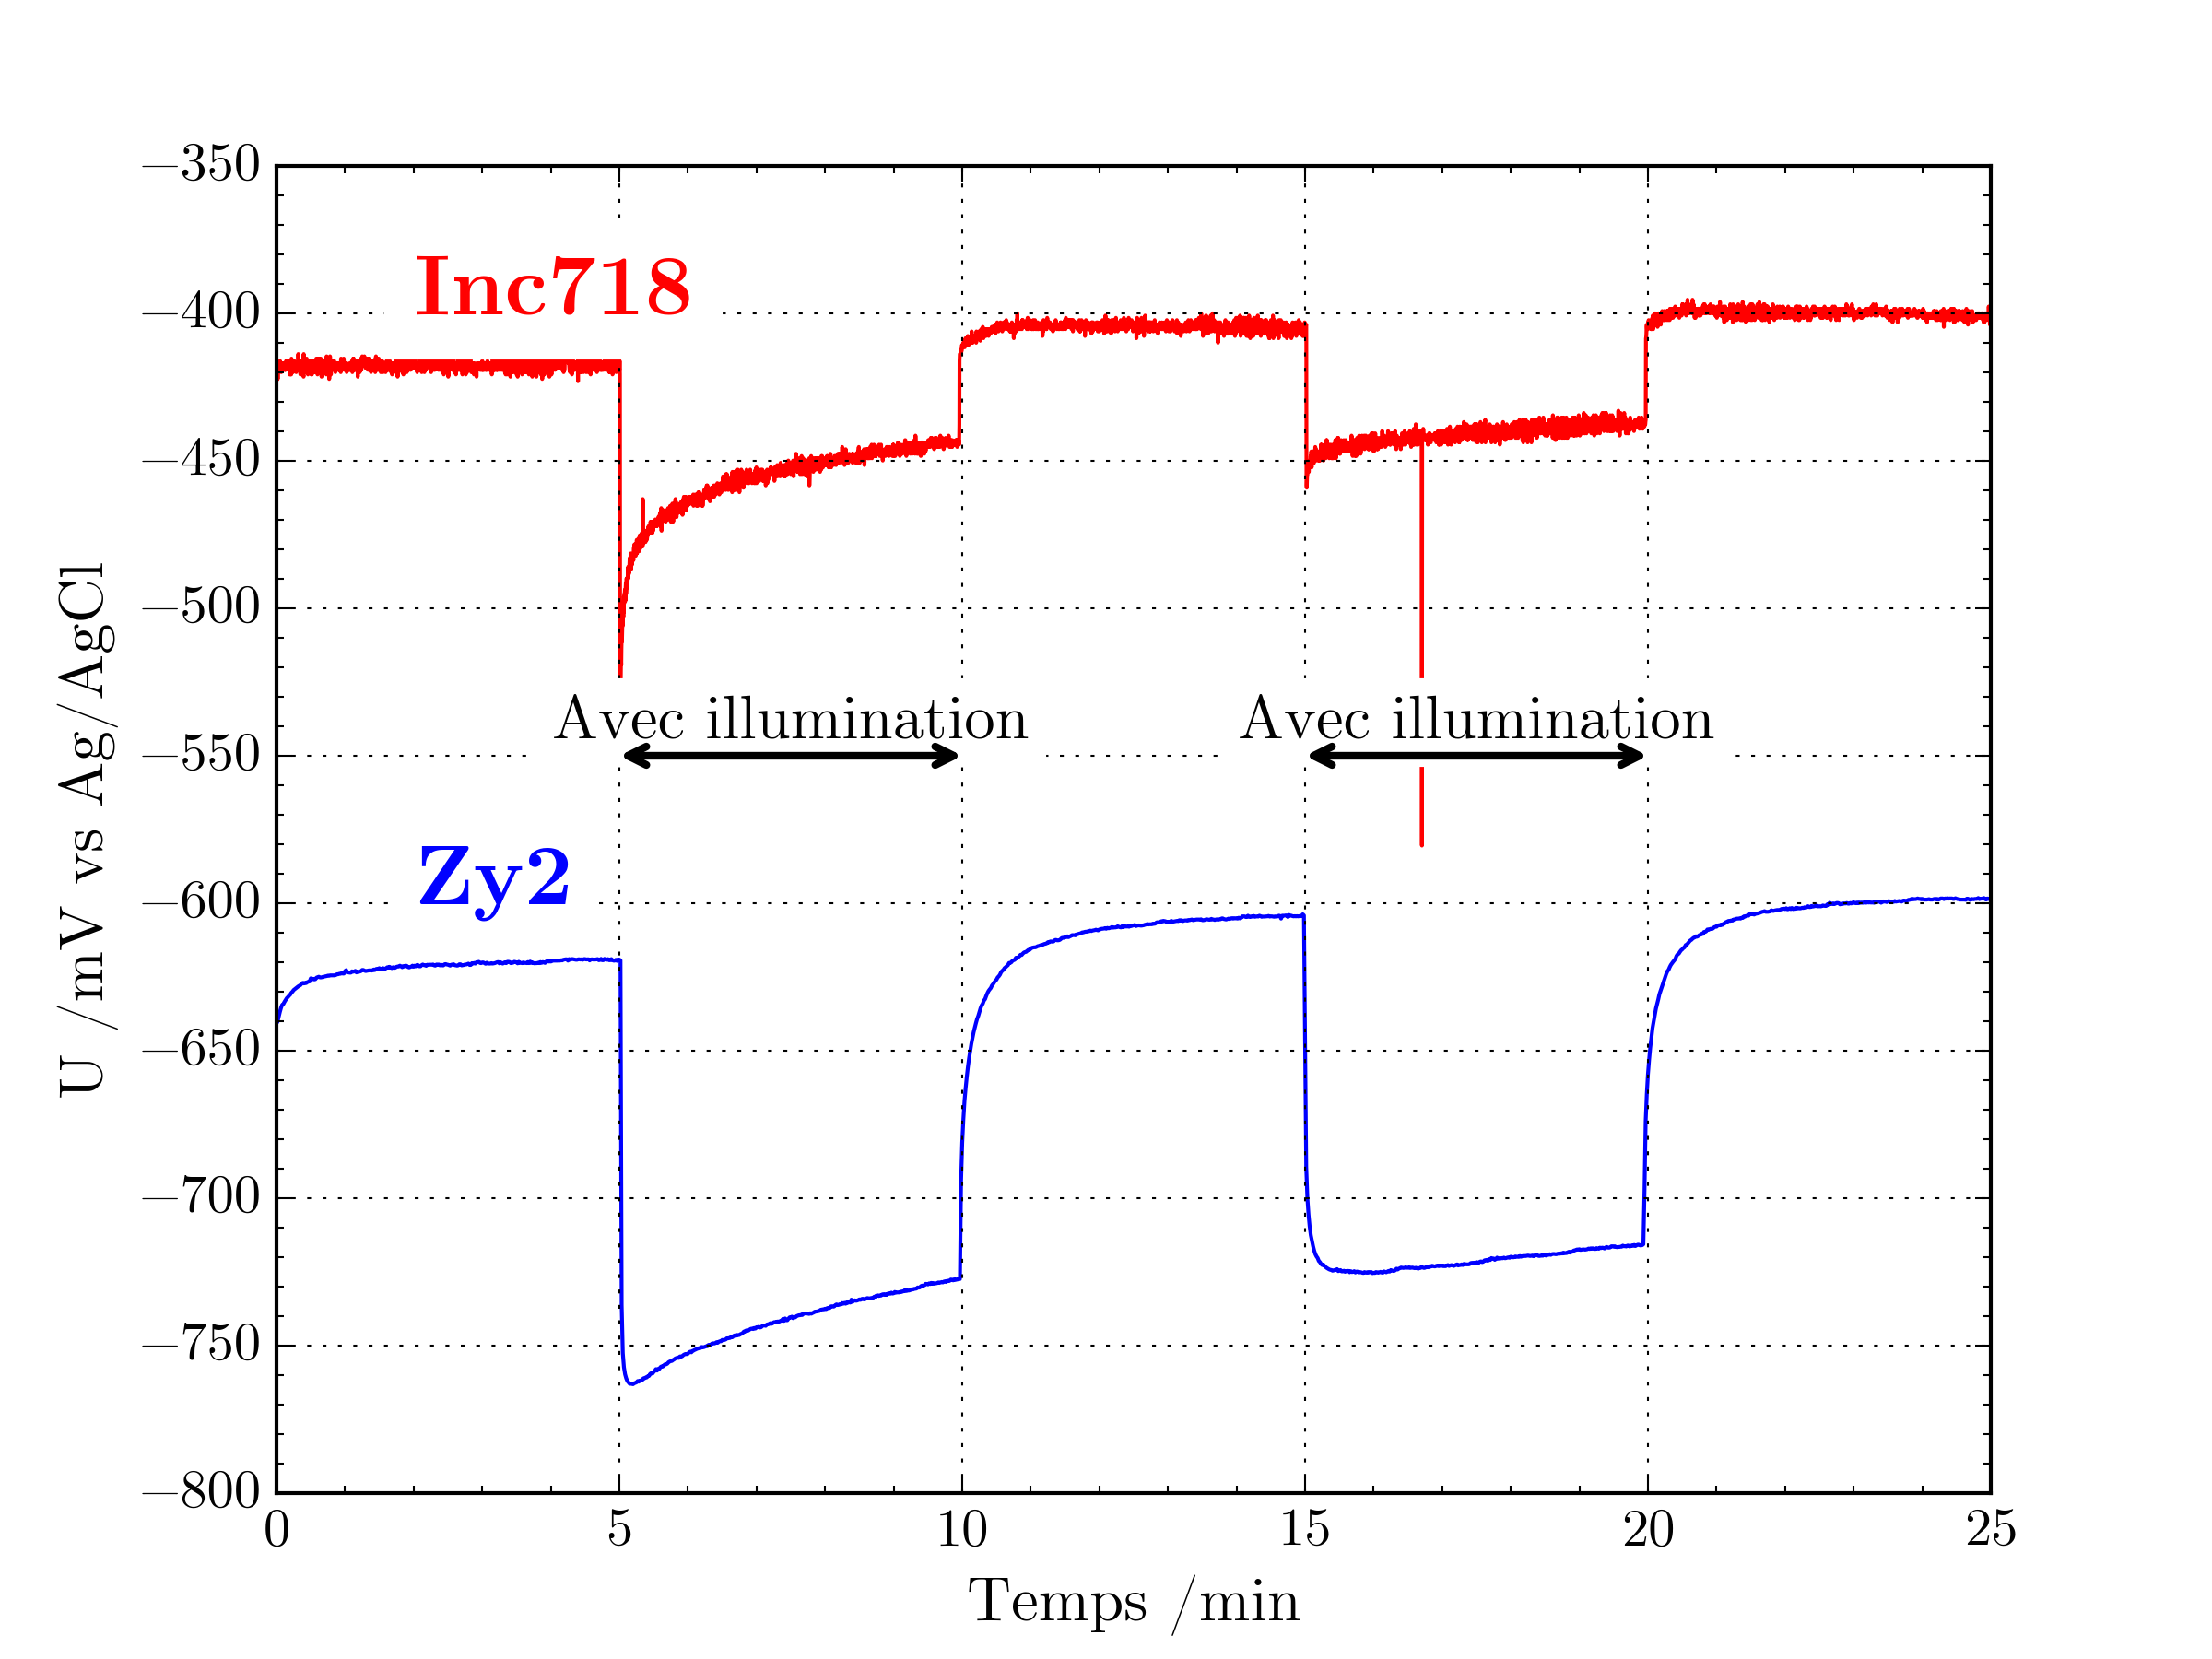
\includegraphics[width=0.65\textwidth]{150215-Illustration-ECP.png}
            \caption{Evolution du potentiel à l'abandon avec et sans illumination UV--Visible intense (lampe Hg) pour les
            alliages Zy2 et Inc718 mesurés avec le nouveau dispositif expérimental.}
            \label{fig:ch3_illustration_ECP}
    \end{figure}

    \begin{figure}[H]
        \centering
            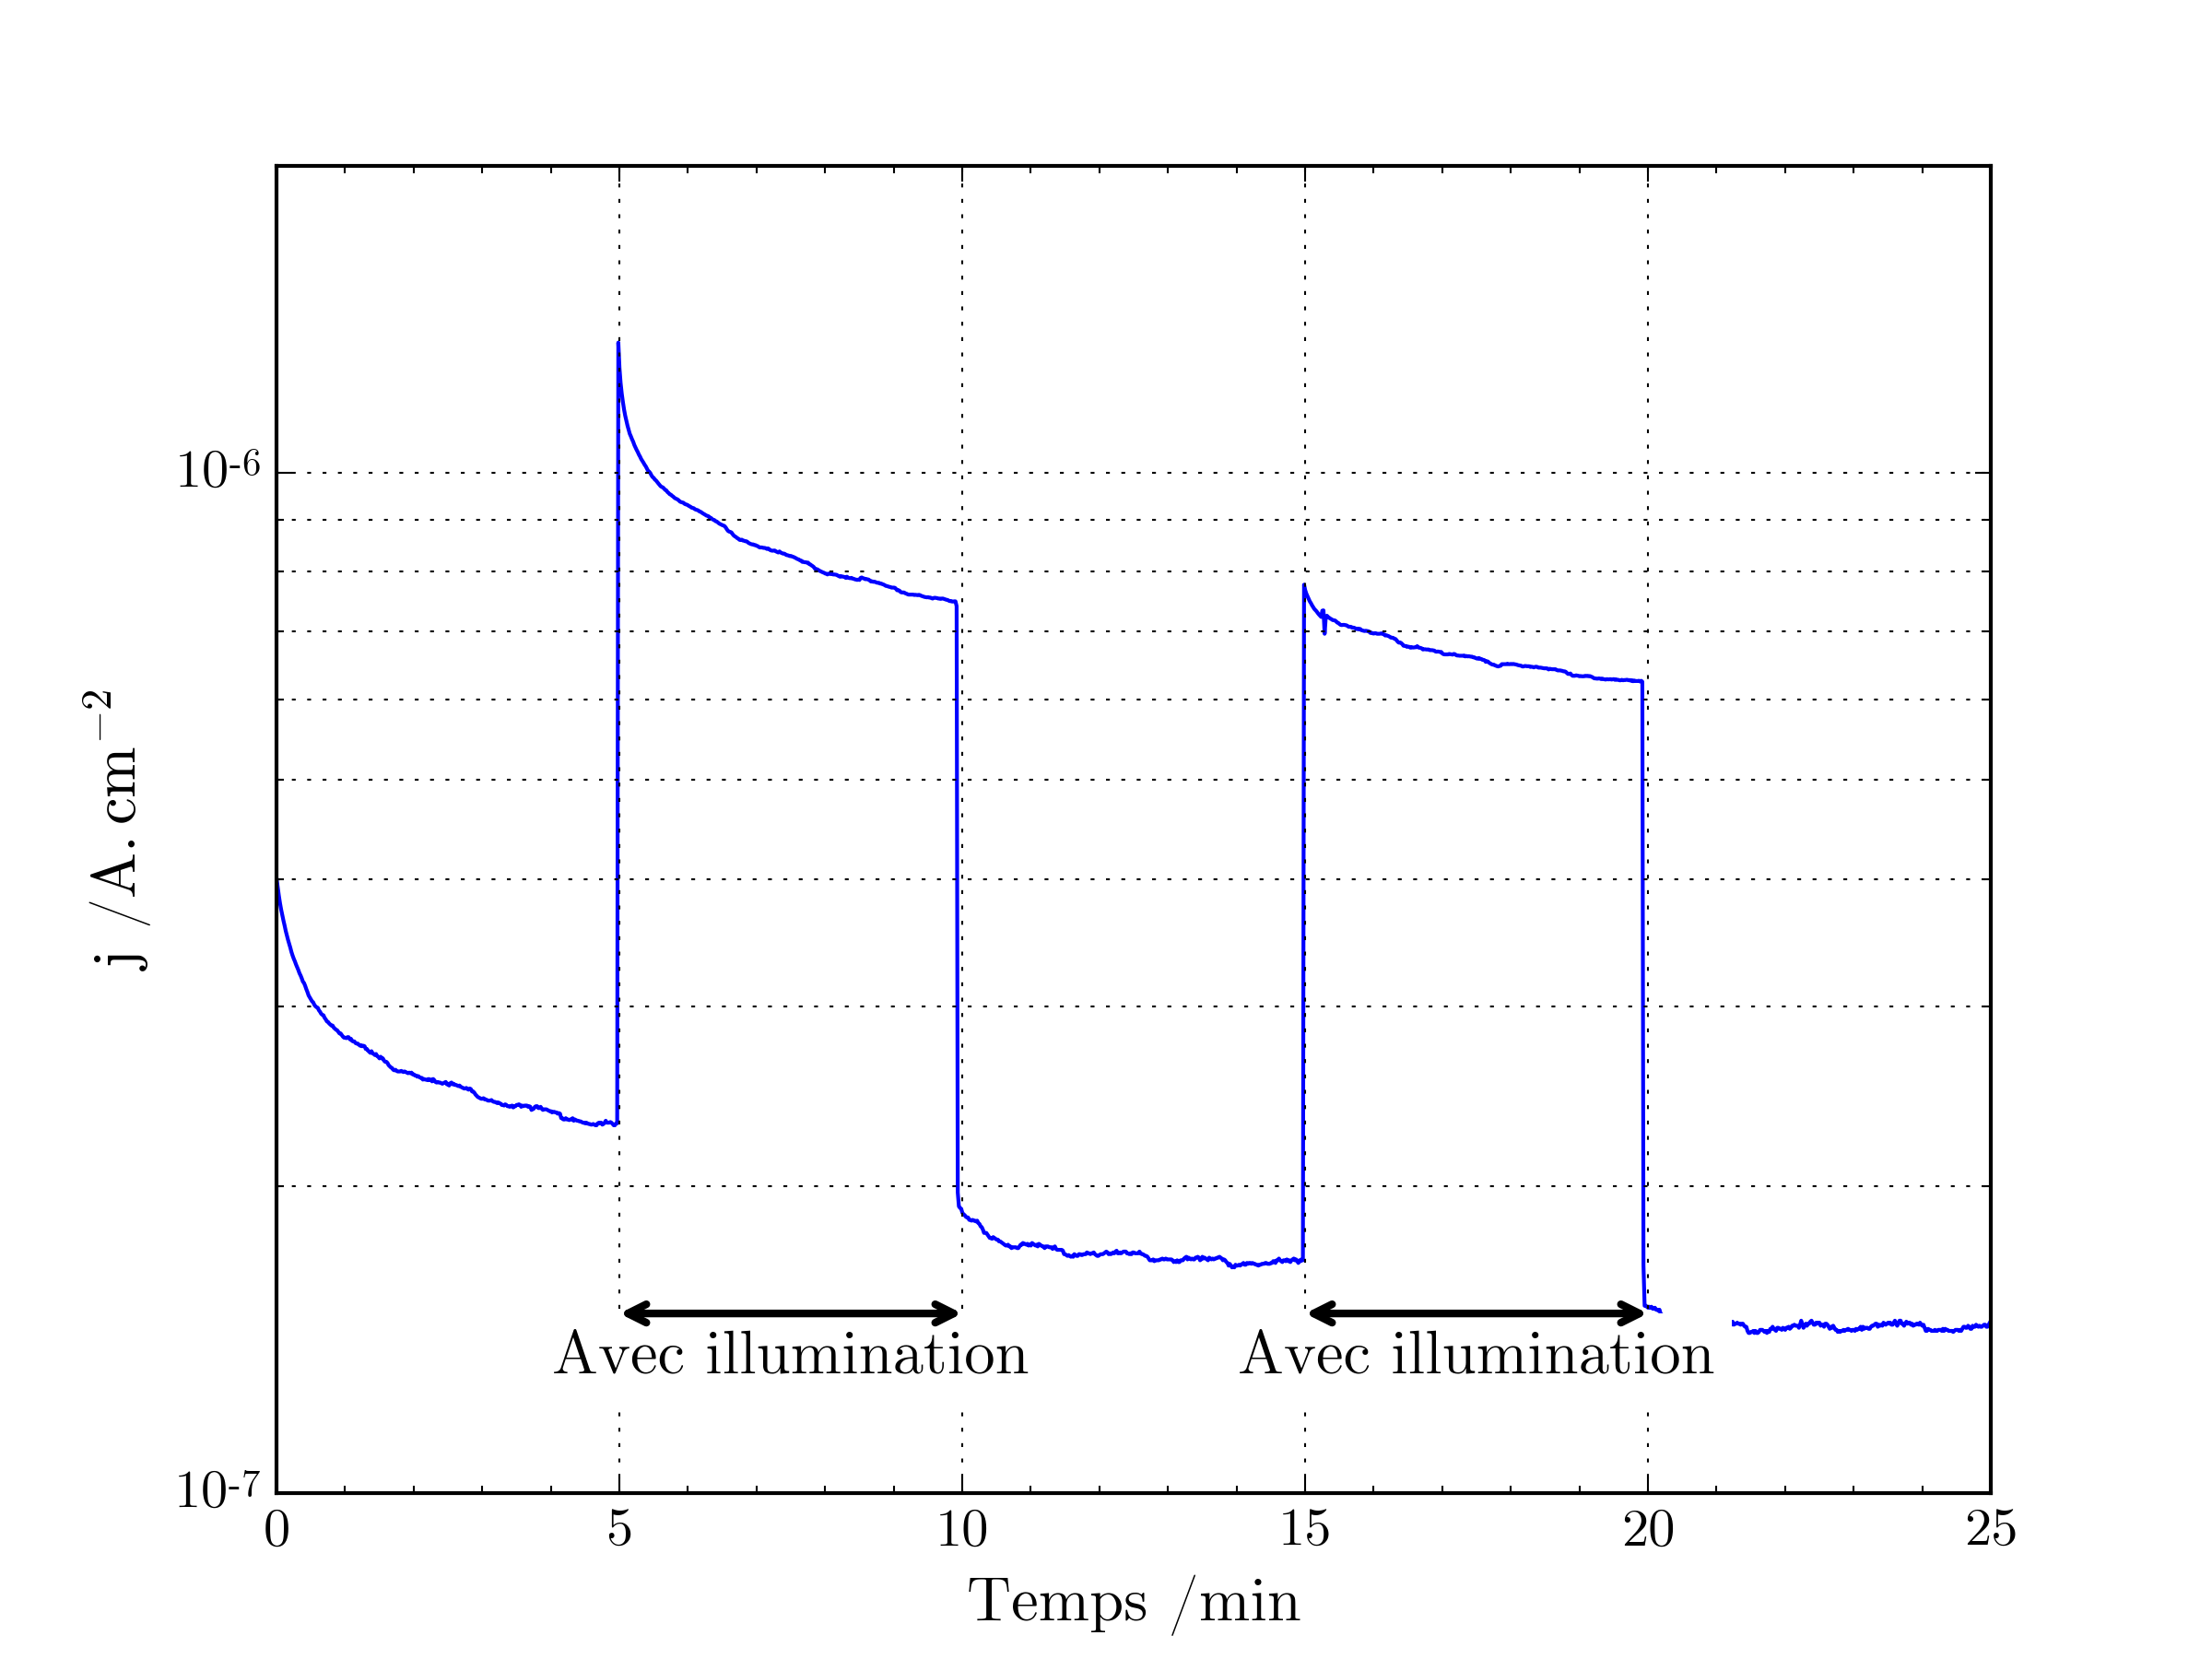
\includegraphics[width=0.65\textwidth]{150215-Illustration-ZRA.png}
            \caption{Evolution de la densité de courant avec et sans illumination UV--Visible intense (lampe Hg) lorsque les
            alliages Zy2 et Inc718 sont en situation de couplage.}
            \label{fig:ch3_illustration_ZRA}
    \end{figure}

    La nouvelle cellule HTP offre aussi la possibilité de mesurer des courbes de polarisation avec et sans
    illumination UV--Visible intense comme illustré en figure \ref{fig:ch3_illustration_polarization_curve}.
    Les courbes de polarisation présentée (corrigées de la résistance d'électrolyte) et normalisées à la surface
    de l'échantillon,
    présentent un niveau de bruit suffisamment bas pour permettre d'estimer la pente de Tafel et la densité de courant d'échange.
     
    \begin{figure}[H]
        \centering
            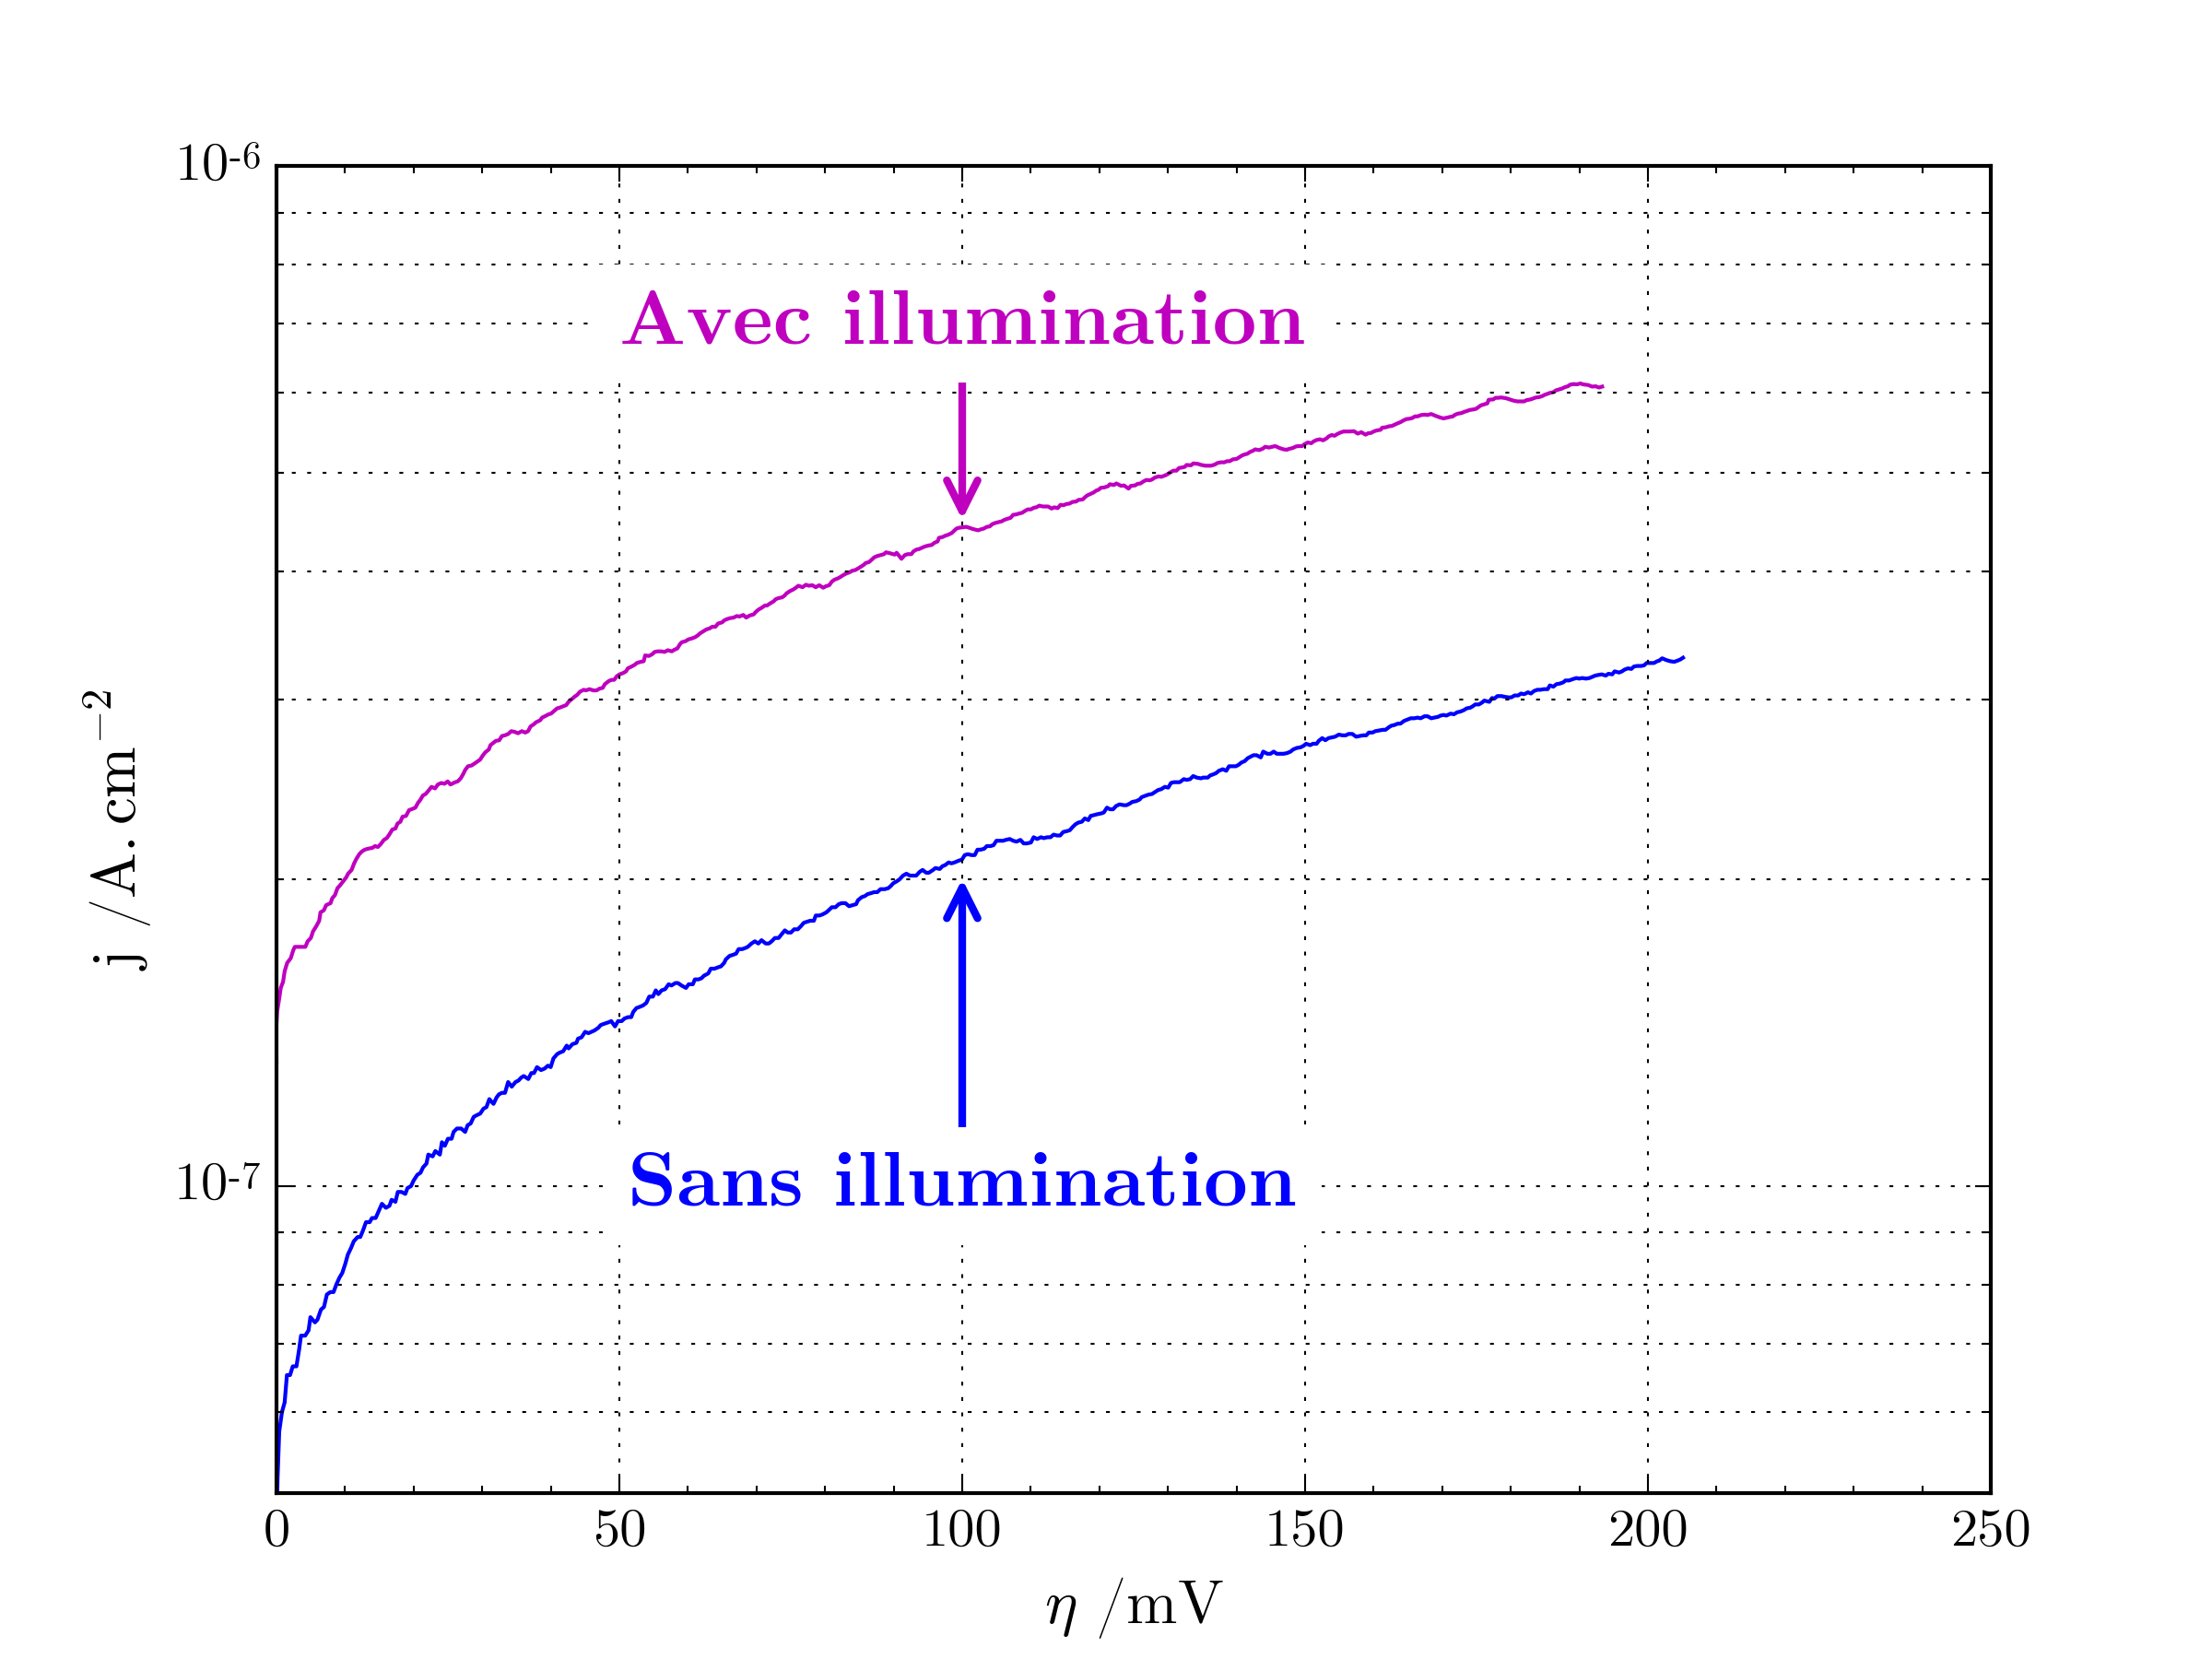
\includegraphics[width=0.65\textwidth]{150215-Illustration-PD-Zy2.png}
            \caption{Courbes de polarisation obtenues sur du Zy2 avec et sans illumination UV--Visible intense (lampe Hg).}
            \label{fig:ch3_illustration_polarization_curve}
    \end{figure}        

    Enfin nous présentons en figure \ref{fig:ch3_ht_pec_example} une photocaractéristique en énergie obtenue avec notre
    dispositif sur l'alliage Zy2 à \SI{280}{\degreeCelsius} et \SI{80}{bars}. 
    La photocaractéristique en énergie, mesurée à température ambiante
    sur le dispositif PEC du laboratoire SIMaP, pour le même échantillon est présentée également, pour mettre en évidence
    le niveau de bruit plus élevé sur le spectre de 
    photocourant mesuré à \SI{280}{\degreeCelsius}. Les deux photocaractéristiques sont normalisées à
    \SI{3.94}{\electronvolt} afin de faciliter la comparaison car les photocourants mesurés ne sont 
    pas du même ordre de grandeur. L'offset artificiel utilisé pour présenter la photocaractéristique obtenue à \SI{280}{\degreeCelsius} permet de
    mieux visualiser l'allure des deux photocaractéristiques.

    \begin{figure}[H]
        \centering
        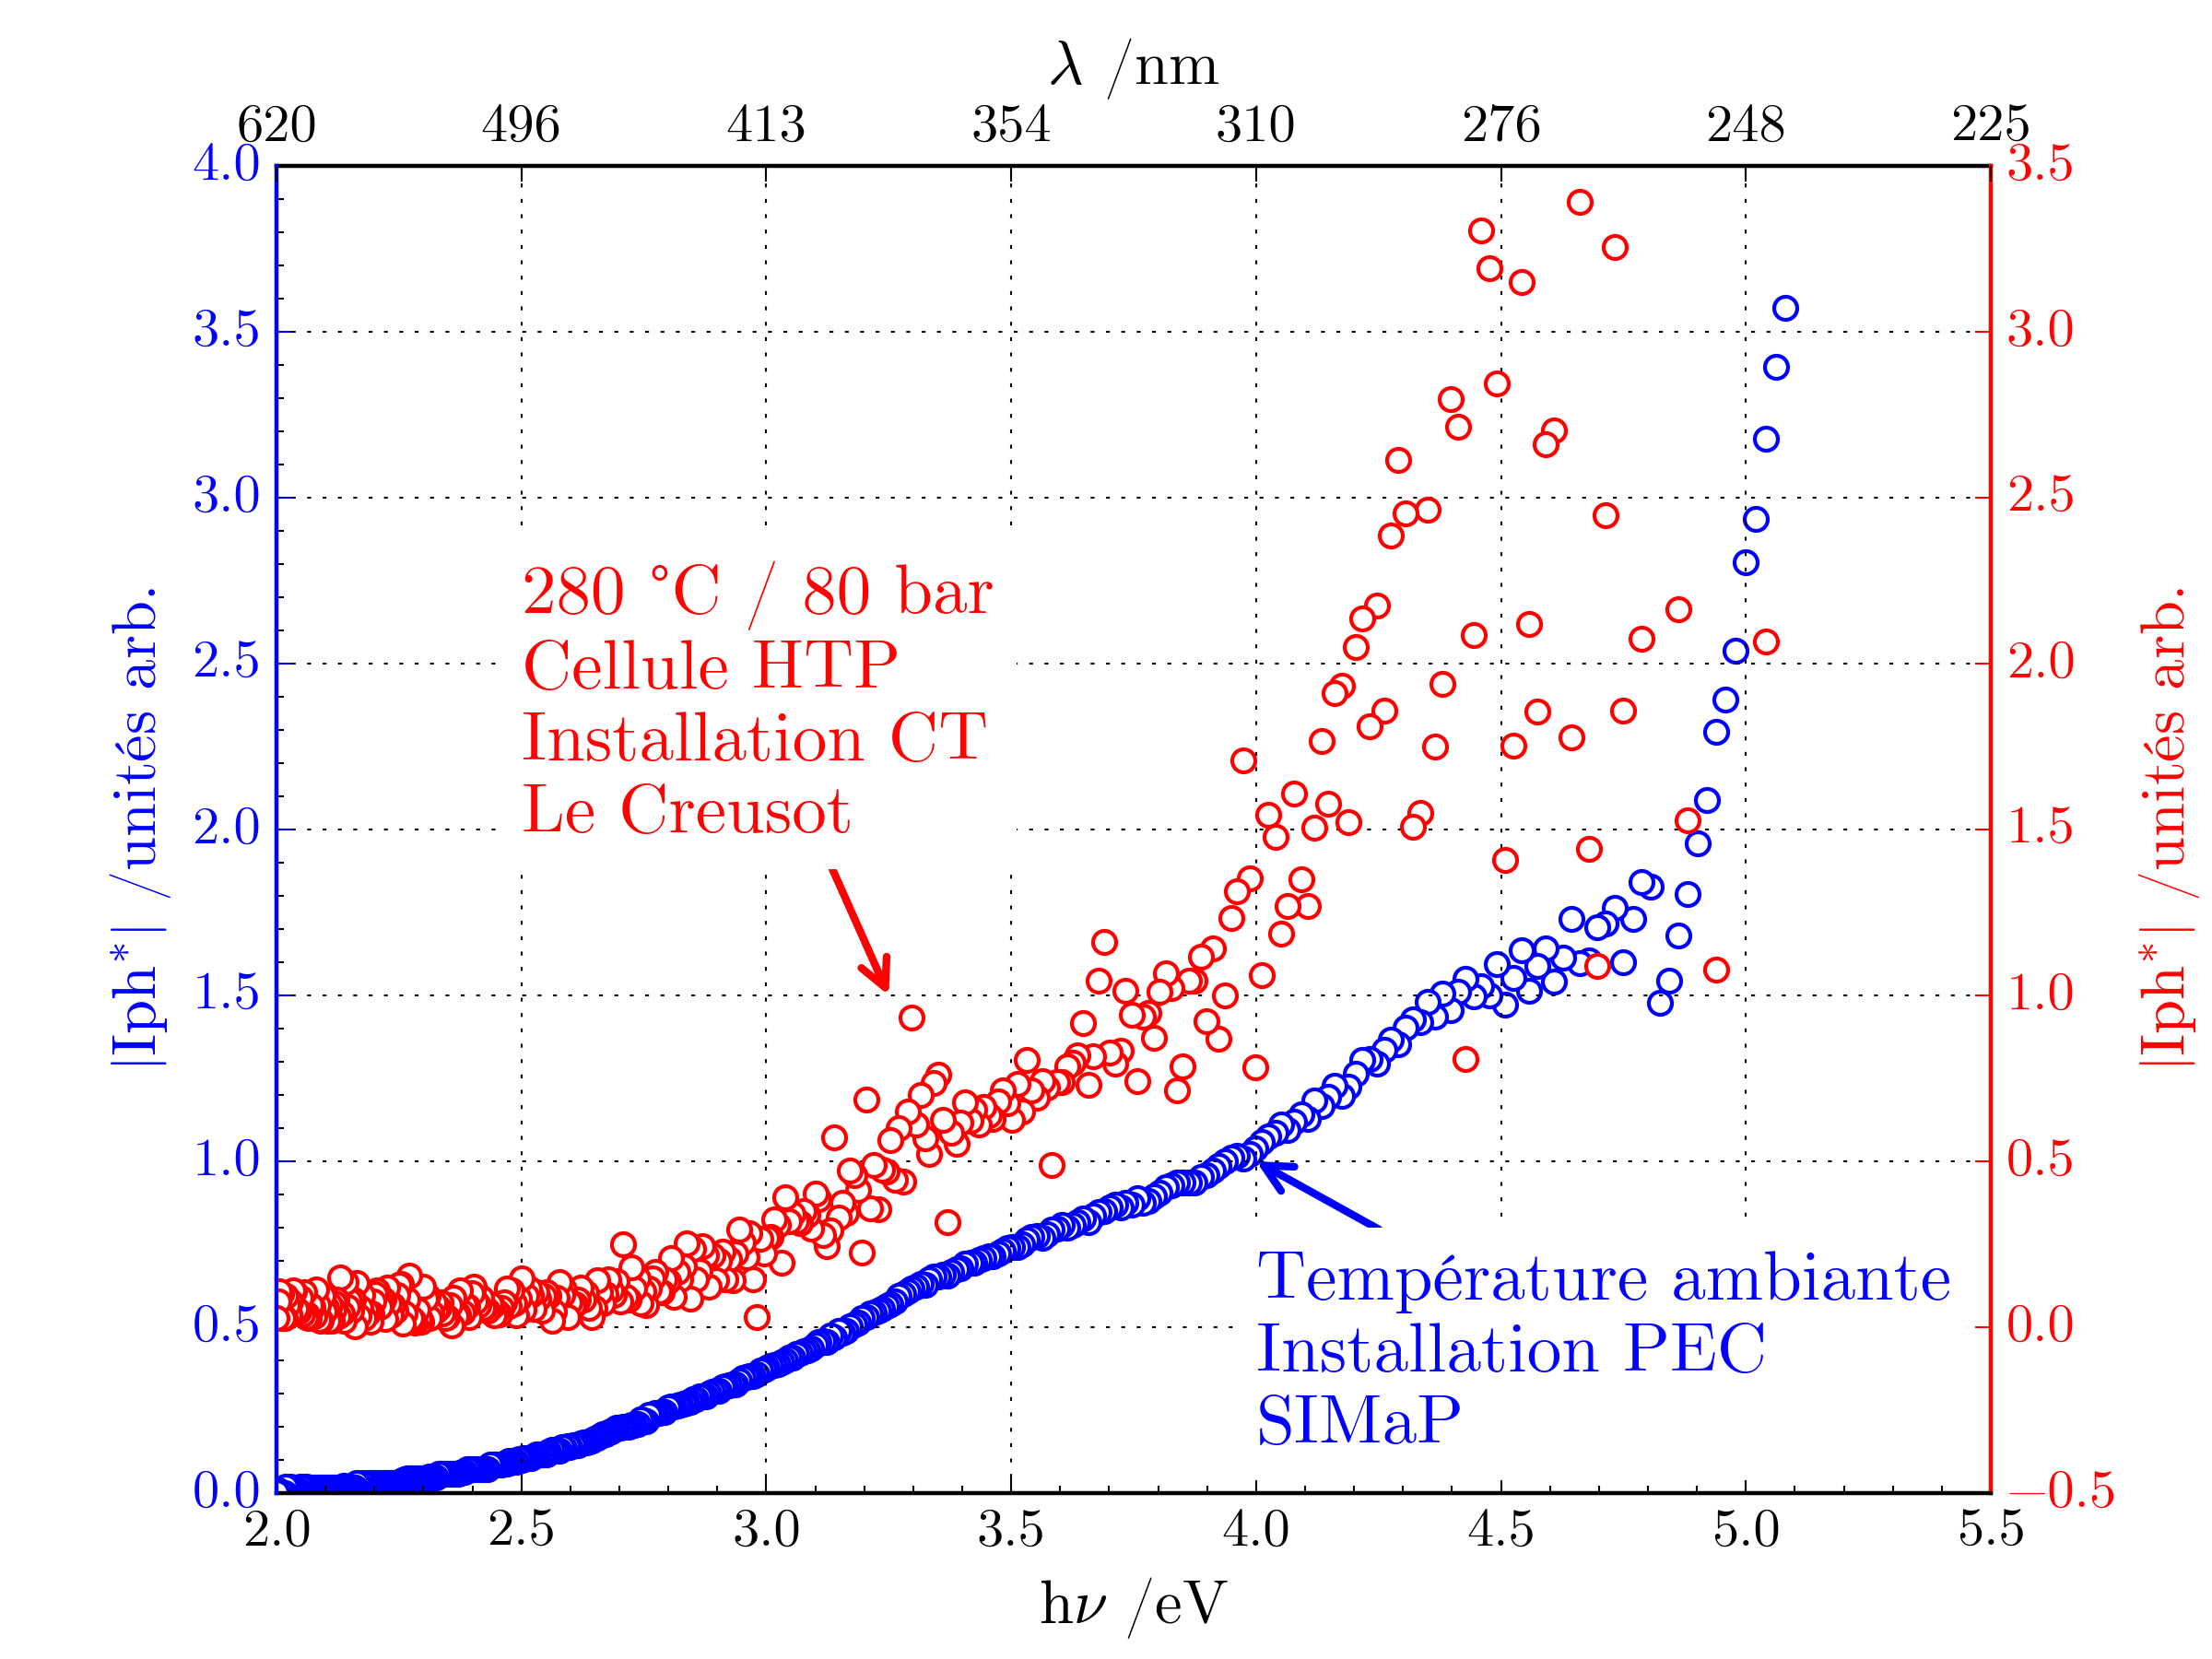
\includegraphics[width=0.65\textwidth]{150215-Illustration-PEC.png}
        \caption{Photocaractéristique en énergie sous illumination modulée (lampe Xe) obtenue sur l'alliage Zy2 avec le
        nouveau dispositif expérimental. Les photocourants ont été normalisés à 1 à 3.94~eV.}
        \label{fig:ch3_ht_pec_example}
    \end{figure}

    Comme vu au chapitre \ref{chap:ch1_bib}
    (\S\ref{subsec:ch1_PEC_applications}),
    \citet{Bojinov2002} ont montré la faisabilité de la caractérisation photoélectrochimique à haute température sur des couches d'oxyde formées sur du
    fer pur (figure \ref{fig:ch3_ht_pec_Bojinov}). Notre cellule HTP
    permet de réaliser des caractérisations photoélectrochimiques à une température supérieure à
    \SI{200}{\degreeCelsius} et de mesurer des photocourants à des énergies allant jusqu'à un peu plus de 5~eV selon les
    échantillons. 
    
    \begin{figure}[H]
        \centering
        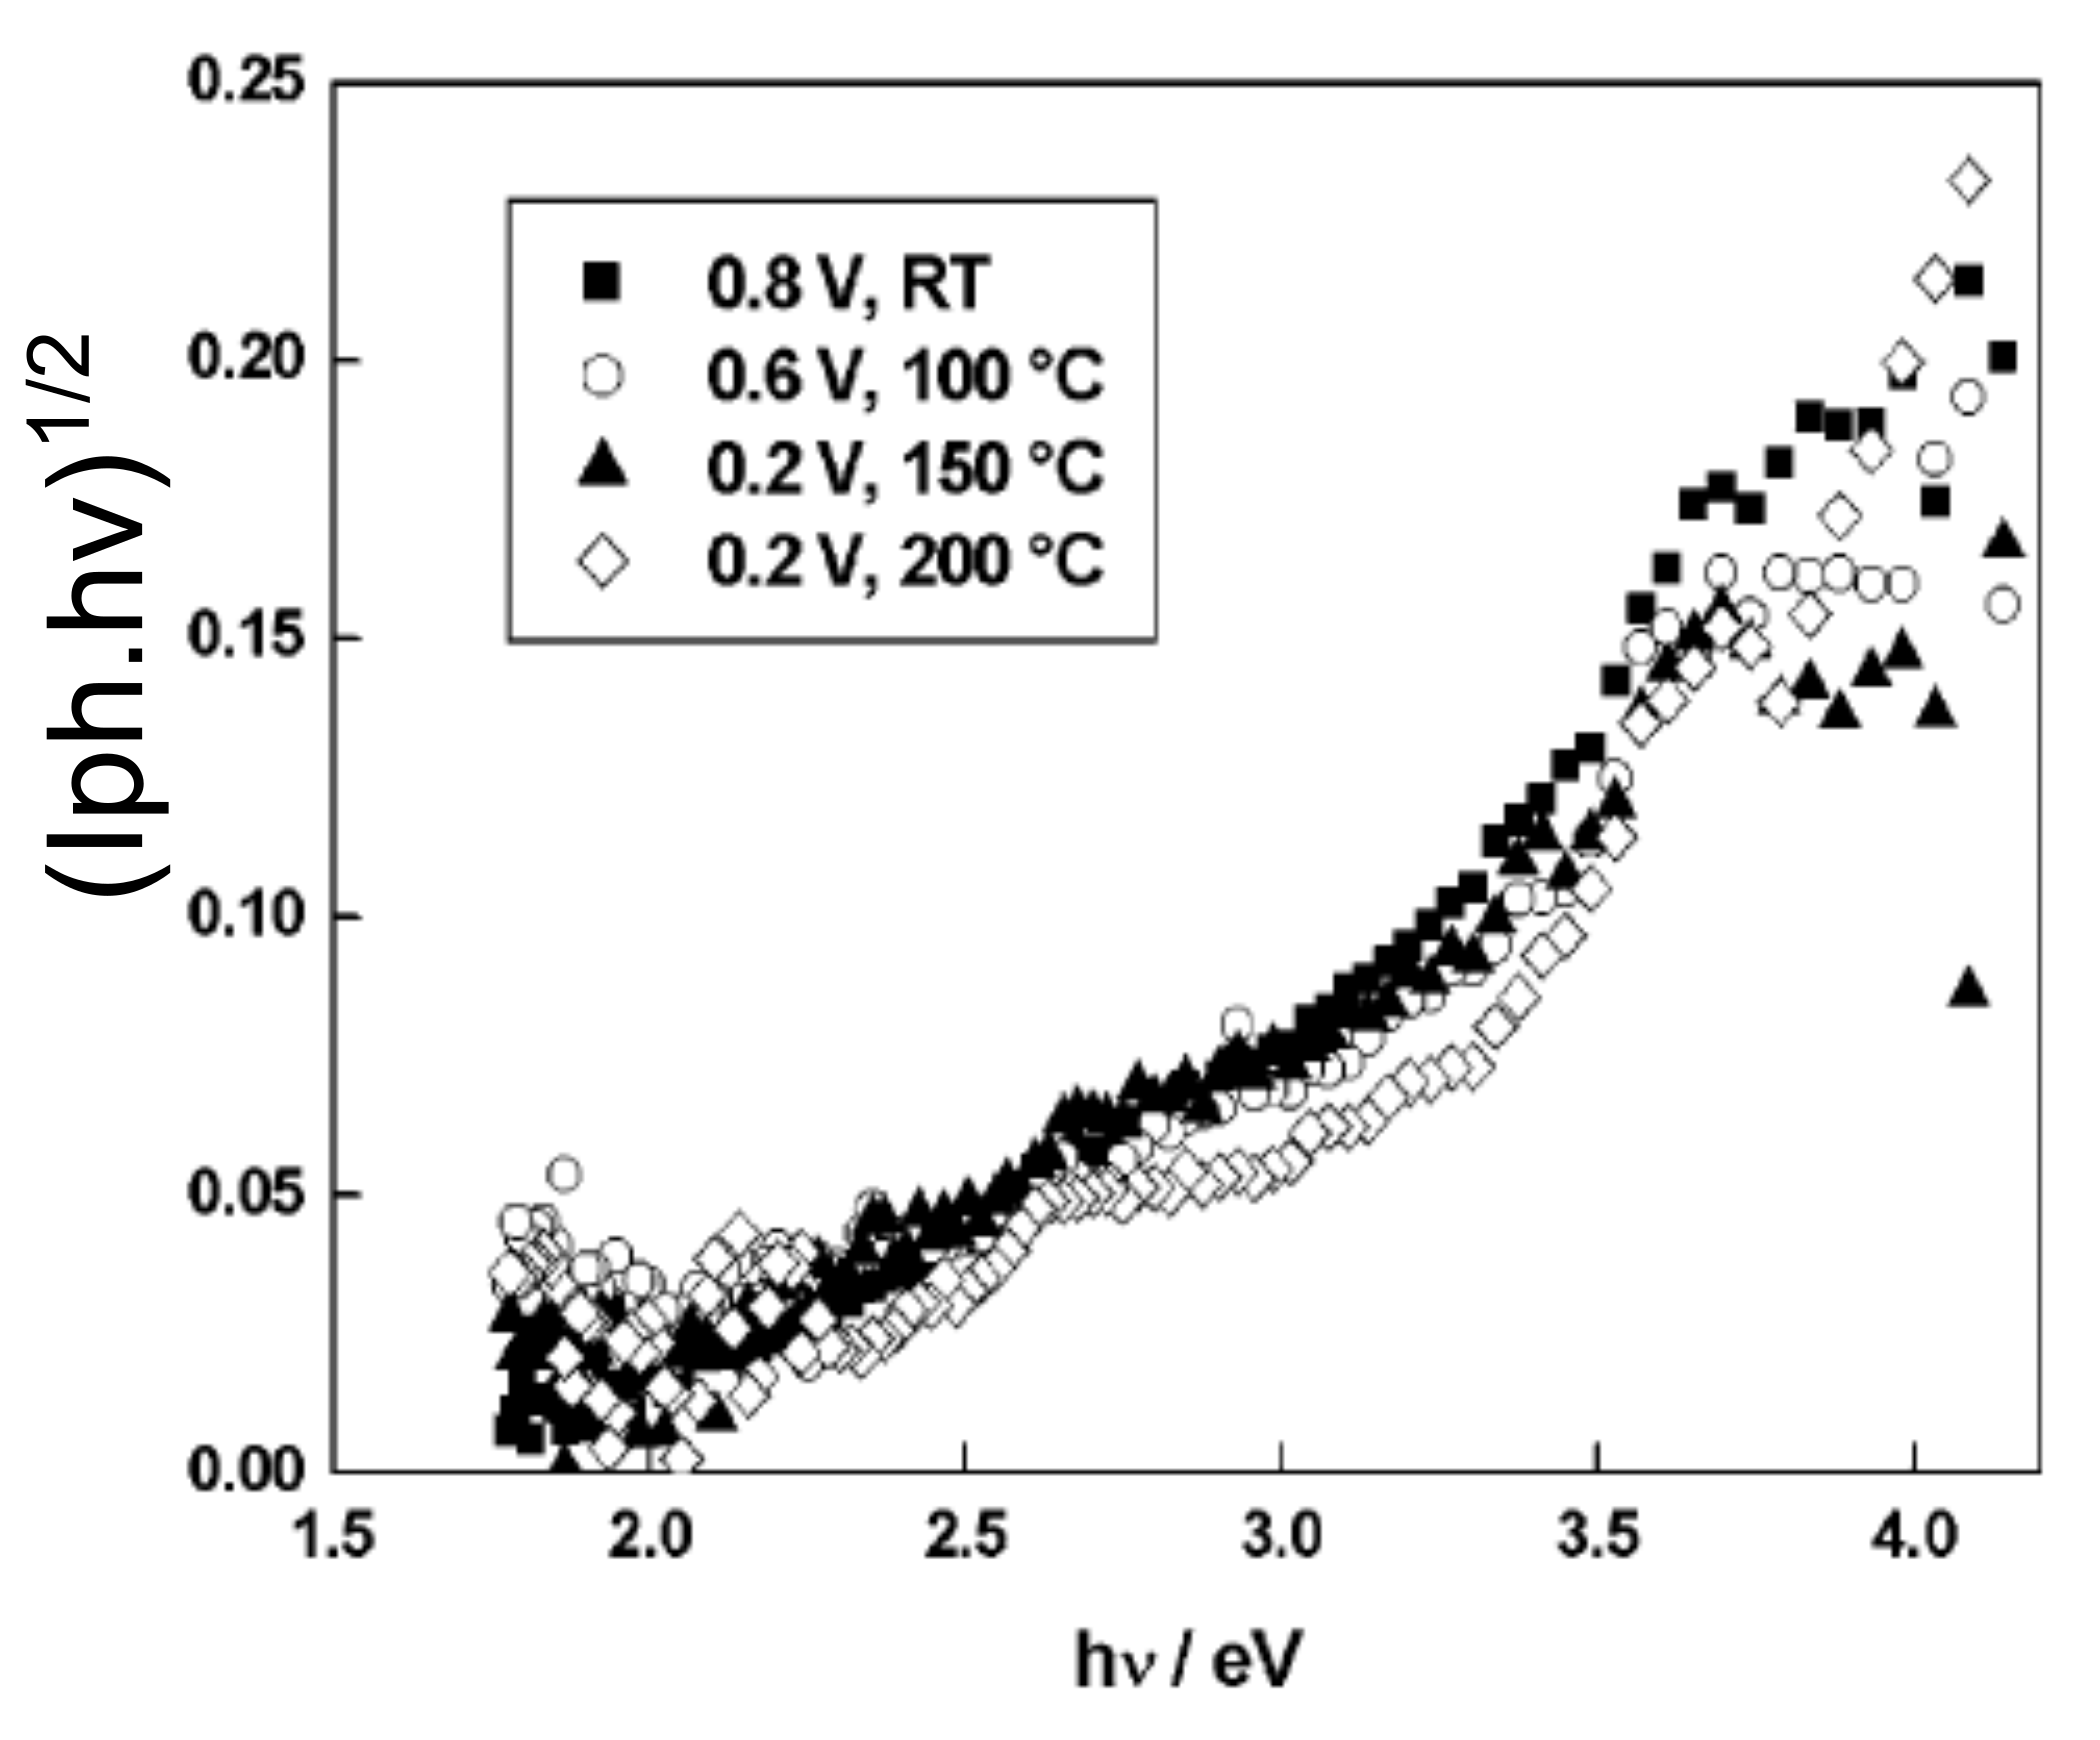
\includegraphics[width=0.65\textwidth]{Bojinov_2002_Fig5b-redraw.png}
        \caption[Transformées linéaires ($IPCE^{1/2}$) des photocaractéristiques en énergie obtenues par M. \textsc{Bojinov} sur du fer pur
        dans 0.05~M de $Na_2B_4O_7$.]
        {Transformées linéaires des photocaractéristiques en énergie obtenues par \citet{Bojinov2002} sur du fer pur
        dans 0.05~M de $Na_2B_4O_7$.}
        \label{fig:ch3_ht_pec_Bojinov}
    \end{figure}

    Les principaux résultats expérimentaux obtenus dans notre dispositif expérimental seront discutés dans le chapitre
    suivant.
\singlespacing
\printbibliography[heading=subbibintoc]
\onehalfspacing
\end{refsection}
